\documentclass[12pt,twoside,titlepage]{report}

%%%%%%%%%%%%%%%%%%%%%%%%%%%%%% Paquetes %%%%%%%%%%%%%%%%%%%%%%%%%%%%%%%%%%%%%

\usepackage[a4paper,bindingoffset=3mm,bottom=35mm]{geometry}
\usepackage[colorlinks=true,pdftex]{hyperref}   %%% Opcional. Para incluir marcadores y enlaces en el pdf
\usepackage[pdftex]{graphicx}  %%% para pdflatex. Las figuras pueden estar en pdf, jpg, svg y otros formatos
\usepackage[spanish]{babel}
%\usepackage[latin1]{inputenc} % Usad en WinEdt/MikTex
\usepackage[utf8]{inputenc} % Usad en overleaf
%\usepackage[T1]{fontenc}
\usepackage{amsmath,amssymb}
\usepackage{hyperref}
\usepackage{color}
\usepackage{afterpage}
\usepackage{paralist}
\usepackage{array}
\usepackage{enumerate}
\usepackage{paralist}
\usepackage{enumitem}
\usepackage{float}
\usepackage{setspace}
\usepackage{listings}
\usepackage{algorithm}
\usepackage{algorithmic}
\usepackage{fancyhdr}
\usepackage{rotating}
\usepackage{multirow}
\usepackage{quotchap}
\usepackage{lipsum}
\usepackage{verbatim} % comentarios
\usepackage{subfig} %subfiguras
\usepackage{wrapfig} %figuras al lado de texto

%%%%%%%%%%%%%%%%%%%%%%% Definiciones básicas %%%%%%%%%%%%%%%%%%%%%%%%%%%%%%%

\newcommand{\nombreautor}{Alberto Gómez Cano}
\newcommand{\nombretutor}{Manuel Rubio Sánchez}
\newcommand{\titulotrabajo}{EARFIT: Aplicación Para Entrenamiento Auditivo Musical}
\newcommand{\escuela}{Escuela Técnica Superior\\de Ingeniería Informática}
\newcommand{\escuelalargo}{Escuela Técnica Superior de Ingeniería Informática}
\newcommand{\universidad}{Universidad Rey Juan Carlos}
\newcommand{\fecha}{\today}
\newcommand{\grado}{Grado en Ingeniería Informática}
\newcommand{\curso}{Curso 2021-2022}
\newcommand{\logoUniversidad}{logoURJC.pdf}
\graphicspath{ {assets} }


% Definiciones de colores (para hidelinks)
\definecolor{BlueLink}{rgb}{0.165,0.322,0.745}
\definecolor{PinkLink}{rgb}{0.8,0.22,0.5}
\definecolor{gray}{rgb}{0.6,0.6,0.6}
% Enlaces
\hypersetup{hidelinks,pageanchor=true,colorlinks,citecolor=PinkLink,urlcolor=black,linkcolor=BlueLink}
\newcommand\blankpage{%
    \newpage
    \null
    \thispagestyle{empty}%
    %\addtocounter{page}{-1}%
    \newpage}
% Texto referencias
\addto{\captionsspanish}{\renewcommand{\bibname}{Bibliografía}}
% Texto Índice de tablas
\addto\captionsspanish{\def\tablename{Tabla}\def\listtablename{\'{I}ndice de tablas}}
\floatname{algorithm}{Algoritmo}
\newfloat{algorithm}{t}{lop}
%\newenvironment{pseudocodigo}[1][htb]
%  {\renewcommand{\algorithmcfname}{Pseudocódig}% Update algorithm name
%   \begin{algorithm}[#1]%
%  }{\end{algorithm}}
  
%%%%%%%%%%%%%%%%%%%%%%% Estilo de código (en Python) %%%%%%%%%%%%%%%%%%%%%%%

\definecolor{bg}{rgb}{0.95,0.95,0.95}
\definecolor{mydeepteal}{rgb}{0.16,0.22,0.23}
\definecolor{myteal}{rgb}{0.31,0.44,0.46}
\definecolor{mymediumteal}{rgb}{0.41,0.58,0.60}
\DeclareFixedFont{\ttb}{T1}{txtt}{bx}{n}{12} % for bold
\DeclareFixedFont{\ttm}{T1}{txtt}{m}{n}{12}  % for normal
%\newcommand*{\FormatDigit}[1]{\textcolor{mydeepteal}{#1}}
\newcommand*{\FormatDigit}[1]{\textcolor{black}{#1}}
% Python style for highlighting
\newcommand\mypythonstyle{\lstset{
language=Python,
basicstyle=\ttfamily\small,
%basicstyle=\linespread{1.0}\footnotesize\ttm,
otherkeywords={self},             % Add keywords here
keywordstyle=\bfseries\ttfamily\color{myteal},
%keywordstyle=\ttb\color{myteal},
commentstyle=\itshape\color{myteal},
stringstyle=\color{mydeepteal},
emph={MyClass,__init__},          % Custom highlighting
emphstyle=\ttb\color{mydeepteal},    % Custom highlighting style
% Any extra options here
showstringspaces=false,            %
backgroundcolor=\color{bg},
rulecolor = \color{bg},
%identifierstyle=\color{deepgreen},
breaklines=true,
numbers=left,
numbersep=5pt,
numberstyle=\tiny,
tabsize=4,
xleftmargin=1em,
frame = single,
framesep = 3pt,
framextopmargin=0pt,
framexbottommargin=0pt,
framexleftmargin=0pt,
framexrightmargin=0pt,
fontadjust=true,
basewidth=0.55em, % compactness of code
upquote=true,
}}
% Python environment
\lstnewenvironment{mypython}[1][]
{
\mypythonstyle
\lstset{#1}
}
{}
\newcommand\mypythonstylenormalinline{\lstset{
language=Python,
basicstyle=\ttfamily\normalsize,
%basicstyle=\linespread{1.0}\footnotesize\ttm,
otherkeywords={self},            % Add keywords here
keywordstyle=\bfseries\ttfamily\color{myteal},
%keywordstyle=\ttb\color{myteal},
commentstyle=\itshape\color{mymediumteal},
stringstyle=\color{mydeepteal},
emph={MyClass,__init__},          % Custom highlighting
emphstyle=\ttb\color{mydeepteal},    % Custom highlighting style
% Any extra options here
showstringspaces=false,            %
backgroundcolor=\color{bg},
rulecolor = \color{bg},
%identifierstyle=\color{deepgreen},
breaklines=false,
numbers=left,
numbersep=5pt,
numberstyle=\tiny,
tabsize=4,
xleftmargin=0em,
frame = single,
framesep = 3pt,
framextopmargin=0pt,
framexbottommargin=0pt,
framexleftmargin=0pt,
framexrightmargin=0pt,
fontadjust=true,
%basewidth=0.55em, % compactness of code
upquote=true,
}}
\newcommand\mypythoninline[1]{{\mypythonstylenormalinline\lstinline!#1!}}

%%%%%%%%%%%%%%%%%%%%% Comandos definidos por el autor %%%%%%%%%%%%%%%%%%%%%%%%

\newcommand{\transpuesta}{\mbox{\tiny $\mathsf{T}$}}
 





%%%%%%%%%%%%%%%%%%%%%%%%%%%%%%%%%%%%%%%%%%%%%%%%%%%%%%%%%%%%%%%%%%%%%%%%%%%%%%
%                           Inicio del documento                             %
%%%%%%%%%%%%%%%%%%%%%%%%%%%%%%%%%%%%%%%%%%%%%%%%%%%%%%%%%%%%%%%%%%%%%%%%%%%%%%
 
\begin{document}
\pagestyle{plain}
  
%%%%%%%%%%%%%%%%%%%%%%%%%%%%%%%%%%%% Portada %%%%%%%%%%%%%%%%%%%%%%%%%%%%%%%%%%
 
% Universidad, Facultad
\begin{titlepage}
\selectlanguage{spanish}
 
% Logo
\begin{center}
\includegraphics[scale=0.7]{\logoUniversidad}
\end{center}
\bigskip
\begin{center}
\begin{LARGE}
\escuela \\
\end{LARGE}
\end{center}
\bigskip
\bigskip

% Grado
\begin{center}
\begin{large}
\textbf{\grado}\\
\end{large}
\end{center}

% Curso
\begin{center}
\begin{large}
\textbf{\curso}\\
\end{large}
\end{center}
\bigskip
\textbf{\begin{center}
\begin{large}
\textbf{Trabajo Fin de Grado}
\end{large}
\end{center}}
\bigskip
\bigskip
\bigskip

% Nombre del TFG
\begin{center}
\textbf{\begin{large}
\MakeUppercase{\titulotrabajo}\\
\end{large}}
\end{center}

% Nombre del autor y Tutor
\vspace{\fill}
\begin{center}
\textbf{Autor: \nombreautor}\\ \smallskip
\textbf{Tutor: \nombretutor}\\
\bigskip

% Fecha
%\textbf{\fecha}\\
\end{center}
\end{titlepage}

% Pagina en blanco
\hypersetup{pageanchor=true}
\normalsize
\afterpage{\blankpage}
 
% Estilo de párrafo de los capítulos
\setlength{\parskip}{0.75em}
\renewcommand{\baselinestretch}{1.25}

% Interlineado simple
\spacing{1}
\pagenumbering{Roman}
\setcounter{page}{2}

%%%%%%%%%%%%%%%%%%%%%%%%%%%%%%%%%%%%%%%%%%%%%%%%%%%%%%%%%%%%%%%%%%%%%%%%%%%%%%%%%%%

 
%%%%%%%%%%%%%%%%%%%%%%%%% Agradecimientos o dedicatoria %%%%%%%%%%%%%%%%%%%%%%%%%%%

\chapter*{Agradecimientos}

Quiero agradecer este TFG a mi familia por siempre estar a mi lado aconsejándome en los momentos más difíciles de mi carrera. 

A mi novia por aguantar mis frustraciones y animarme a seguir adelante. 

A mi tutor académico Manuel Rubio Sánchez que me ha apoyado para realizar este trabajo. 

Y finalmente, me gustaría agradecer a todos mis compañeros que han compartido esta carrera conmigo.

¡A todos, mil gracias!
\afterpage{\blankpage}

%%%%%%%%%%%%%%%%%%%%%%%%%%%%%%%%%%%%%%%%%%%%%%%%%%%%%%%%%%%%%%%%%%%%%%%%%%%%%%%%%%%

 
%%%%%%%%%%%%%%%%%%%%%%%%%%%%%%%%%%%% Resumen %%%%%%%%%%%%%%%%%%%%%%%%%%%%%%%%%%%%%%

\chapter*{Resumen}
La idea consiste en desarrollar una herramienta para ayudar a músicos a desarrollar su oído (Musical Ear Training). Por ejemplo, para identificar notas, intervalos y escalas. Estos ejercicios mejorarán su capacidad musical al desarrollar una comprensión más intuitiva de lo que se escucha.

Consistirá en una aplicación web basada Next.js y TypeScript y que será desplegada en Vercel. Utilizando Metodologías Ágiles y prácticas de DevOps para llevar a cabo la organización y el desarrollo del producto. Además de Design Thinking y Lean Startup para la ideación, diseño y creación de la solución.

La aplicación se basa en un conjunto de ejercicios de entrenamiento musical divididos en la identificación de notas, intervalos y escalas. Donde los usuarios tratarán de adivinar el sonido de cada ejercicio al pulsar el botón de pregunta. Además, los usuarios cuentan con las posibilidad de personalizar estos ejercicios, variar el instrumento que suena, así como de tocar un pequeño piano para ayudarse en la obtención de sus respuestas.

Todo ello en una aplicación con renderizado en el lado del servidor que tiene como nombre Earfit y se puede visitar en el siguiente enlace:

\url{https://earfit-alberttogoca.vercel.app/}

\mbox{} \bigskip

% Palabras Clave
\noindent \textbf{Palabras clave}:
\begin{compactitem}
    \item Entrenamiento Auditivo
    \item Nextjs
    \item React
    \item TypeScript
    \item Vercel
    \item Agile
\end{compactitem}

\afterpage{\blankpage}

%%%%%%%%%%%%%%%%%%%%%%%%%%%%%%%%%%%%%%%%%%%%%%%%%%%%%%%%%%%%%%%%%%%%%%%%%%%%%%%%%%%

 
%%%%%%%%%%%%%%%%%%%%%%%%%%%%%%%%%%%% Índices %%%%%%%%%%%%%%%%%%%%%%%%%%%%%%%%%%%%

% Estilo de párrafo de los Índices
\setlength{\parskip}{1pt}
\renewcommand{\baselinestretch}{1}
\renewcommand{\contentsname}{Índice de contenidos}

% Índice de contenidos
\tableofcontents
\afterpage{\blankpage}

% Índice de figuras (OPCIONAL)
\listoffigures
\afterpage{\blankpage}
\addcontentsline{toc}{chapter}{\listfigurename}

% Índice de códigos/algoritmos (OPCIONAL).   El término "Códigos" se puede cambiar por "Métodos", "Funciones", "Algoritmos", etc.
\renewcommand\lstlistlistingname{Códigos}
\renewcommand\lstlistingname{Código}
\renewcommand\lstlistlistingname{Índice de códigos}

\lstlistoflistings
\afterpage{\blankpage}
\addcontentsline{toc}{chapter}{\lstlistlistingname}


%%%%%%%%%%%%%%%%%%%%%%%%%%%%%%%%%%%%%%%%%%%%%%%%%%%%%%%%%%%%%%%%%%%%%%%%%%%%%%%%%%%
  

%%%%%%%%%%%%%%%%%%%%%%% Cabeceras y pies de página (Opcional) %%%%%%%%%%%%%%%%%%%%%%%

%\setlength{\headheight}{15.2pt}
\pagestyle{fancy}
\renewcommand{\chaptermark}[1]{\markboth{Capítulo \thechapter.\ #1}{}}
\pagestyle{fancy}
\fancyhf{}
\fancyhead[LO]{\leftmark}
\fancyhead[RO]{}
\fancyhead[RE]{\nouppercase\rightmark}
\fancyhead[LE]{}
\fancyfoot[C]{\thepage}

%%%%%%%%%%%%%%%%%%%%%%%%%%%%%%%%%%%%%%%%%%%%%%%%%%%%%%%%%%%%%%%%%%%%%%%%%%%%%%%%%%%%

   
%%%%%%%%%%%%%%%%%%%%%%%%%%%%%% Capítulos de la memoria %%%%%%%%%%%%%%%%%%%%%%%%%%%%%


%%%%%%%%%%%%%%%%%%%%%%%%%%%%%% 1 Introducción %%%%%%%%%%%%%%%%%%%%%%%%%%%%%%%%%%%%%
\chapter{Introducción}

En este capítulo daremos un poco de explicación sobre qué consiste el entrenamiento auditivo para que pueda comprender mejor el objetivo general y alcance del trabajo. Además, se realizará una pequeña descripción del proyecto y se comentará brevemente el estado del arte actual. Por último, se establecerán los objetivos y la estructura del documento.

% Estilo resto de páginas
\pagestyle{fancy}

% Estilo de párrafo de los capítulos
\setlength{\parskip}{0.75em}
\renewcommand{\baselinestretch}{1.25}

% Interlineado simple
\spacing{1}

% Numeración contenido
\pagenumbering{arabic}
\setcounter{page}{1}

\section{Entrenamiento Auditivo}

Los oídos son la herramienta más importante a la hora de hacer música. Pero si no se entrenan, nunca desarrollarán toda su potencia. Los músicos, productores y DJs se pueden beneficiar del entrenamiento de sus oídos. Puede resultar muy útil a la hora de mezclar música y componer canciones.

El entrenamiento auditivo es el proceso de identificar los elementos de la música en su forma más sencilla y conectarlos con la forma en que sentimos el sonido físicamente. Tradicionalmente, el entrenamiento auditivo para los músicos incluye habilidades como identificar intervalos o escalas. 

Muchas personas suponen que tener “oído musical” es tener la capacidad de identificar una nota al oírla. Tener oído musical es, también, ser capaz de escuchar y comprender música interiormente, sin que ésta este físicamente presente, igual que reflexionamos sobre palabras que hemos escuchado.

El entrenamiento auditivo es importante porque la escucha es una habilidad, al igual que tocar el piano. Por ejemplo, las melodías son simplemente series de intervalos. Con el entrenamiento necesario para identificar los intervalos, se puede aprender a tocar una melodía de oído.

Para los productores de música y DJs, el entrenamiento auditivo sirve para identificar los rangos de frecuencias más rápidamente y ayudarlos también a conseguir los efectos buscados.

En conclusión, aprender entrenamiento auditivo te lleva al siguiente nivel como músico ya que te permite sacar canciones más rápido, con mayor precisión, improvisar mejor, llevar al instrumento las melodías que imaginas con mayor facilidad, y en general te permitirá ser mucho mejor músico.

\subsection{Oído Absoluto}

Es la habilidad para reconocer notas musical sin tener otras como referencia. Es relativamente raro encontrar personas con oído absoluto. Se considera que menos del uno por ciento de la población tiene oído absoluto. Las posibilidades de tener oído absoluto aumentan si has recibido mucho entrenamiento musical desde muy pequeño.

\subsection{Oído Relativo}

Es la habilidad para reconocer notas musical relacionándolas entre sí. Es una habilidad indispensable para los músicos y es más sencilla de entrenar que el oído absoluto. Esta característica te puede permitir, por ejemplo, interpretar canciones sin disponer de partitura.

Las personas que disponen de oído relativo son capaces de:
\begin{compactitem}
    \item Denotar la distancia de una nota musical desde una nota de referencia establecida.
    \item Seguir la notación musical, esto permite cantar correctamente una melodía entonando cada nota de acuerdo a la distancia con la nota anterior.
    \item Identificar intervalos entre notas dadas, de manera independiente a la afinación elegida.
\end{compactitem}

Los ejercicios más comunes de entrenamiento auditivo te ayudarán a desarrollar tu oído relativo.

\section{Estado del Arte}

En la actualidad ya existen algunas aplicaciones que contemplan el entrenamiento auditivo como pueden ser ToneGym, TonedEar y EarMaster. En esta sección vamos a analizar cada una de ellas con el objetivo de obtener información útil para nuestra aplicación. Vamos a centrarnos en descubrir los pros y los contras de cada una, que tendremos en cuenta en la fase de ideación y diseño, para mejorar nuestra solución.

\subsection{ToneGym}

Esta aplicación cuenta con los ejercicios clásicos de entrenamiento musical. Una vez en un ejercicio cuenta con varios tipos del mismo y un menú siempre visible a la izquierda para que puedas moverte entre ellos fácilmente. Cuando aciertas la respuesta en un ejercicio recibes un feedback del botón como correcto mediante sonido, el botón se vuelve verde unos segundos y automáticamente se pasa al siguiente sonido, lo que agiliza la práctica.

\begin{figure}[H] 
    \includegraphics[scale=0.25]{Estado del Arte/tonegym}
    \centering
    \label{fig:tonegym}
    \caption{ToneGym}
\end{figure}

Sin embargo, lo primero que vemos al entrar en la aplicación es una landing page en la que si pulsas Lets Start Training nos lleva a crearnos una cuenta en lugar de a los ejercicios. Esto es algo que echa para atrás a probar una aplicación que no conoces. 

\begin{figure}[H]
    \centering
     \subfloat[ToneGym Landing Page]{
      \label{f:tonegymmain2}
       \includegraphics[width=0.45\textwidth]{Estado del Arte/tonegymmain2}}
     \subfloat[ToneGym Login]{
      \label{f:tonegymlogin}
       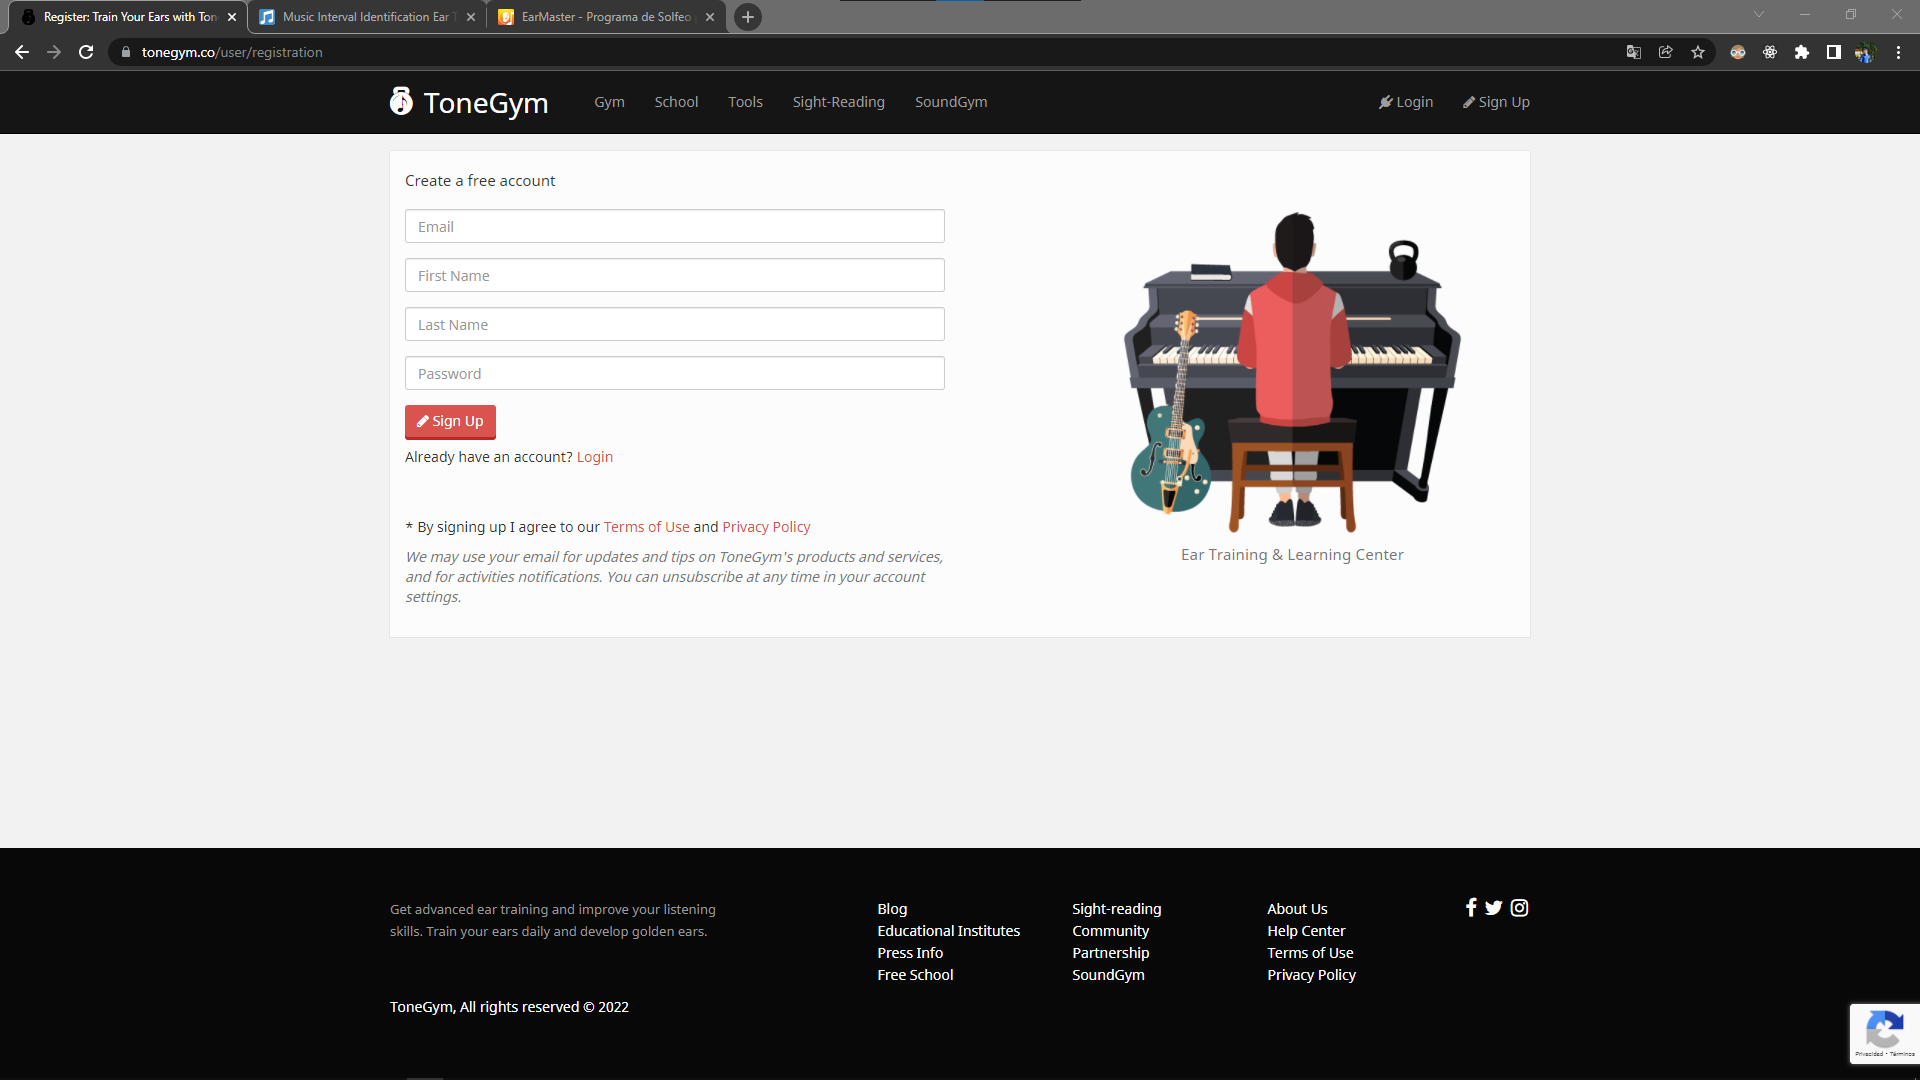
\includegraphics[width=0.45\textwidth]{Estado del Arte/tonegymlogin}}
    \caption{ToneGym}
    \label{f:ToneGym2}
   \end{figure}

La sección de ejercicios esta un poco escondida y hay que deslizar hacia abajo para encontrarla. Aunque el diseño está bastante bien, la personalización de los ejercicios es nula. Además, una vez hayas fallado en la respuesta no se te permite continuar probando. Por último, no incorpora ninguna opción para cambiar el instrumento que suena.

\subsection{TonedEar}

Esta aplicación es la que más se parece a lo que queremos construir. Contiene varios tipos de ejercicios como identificación de intervalos, escalas, etc. Permite la personalización de los ejercicios mediante un panel a la derecha, aunque no es inmediato. Y ofrece la posibilidad de continuar con el ejercicio aunque falles en la primera respuesta. Además, es una aplicación web gratuita, sencilla, fácil de entender y usar.

\begin{figure}[H] 
    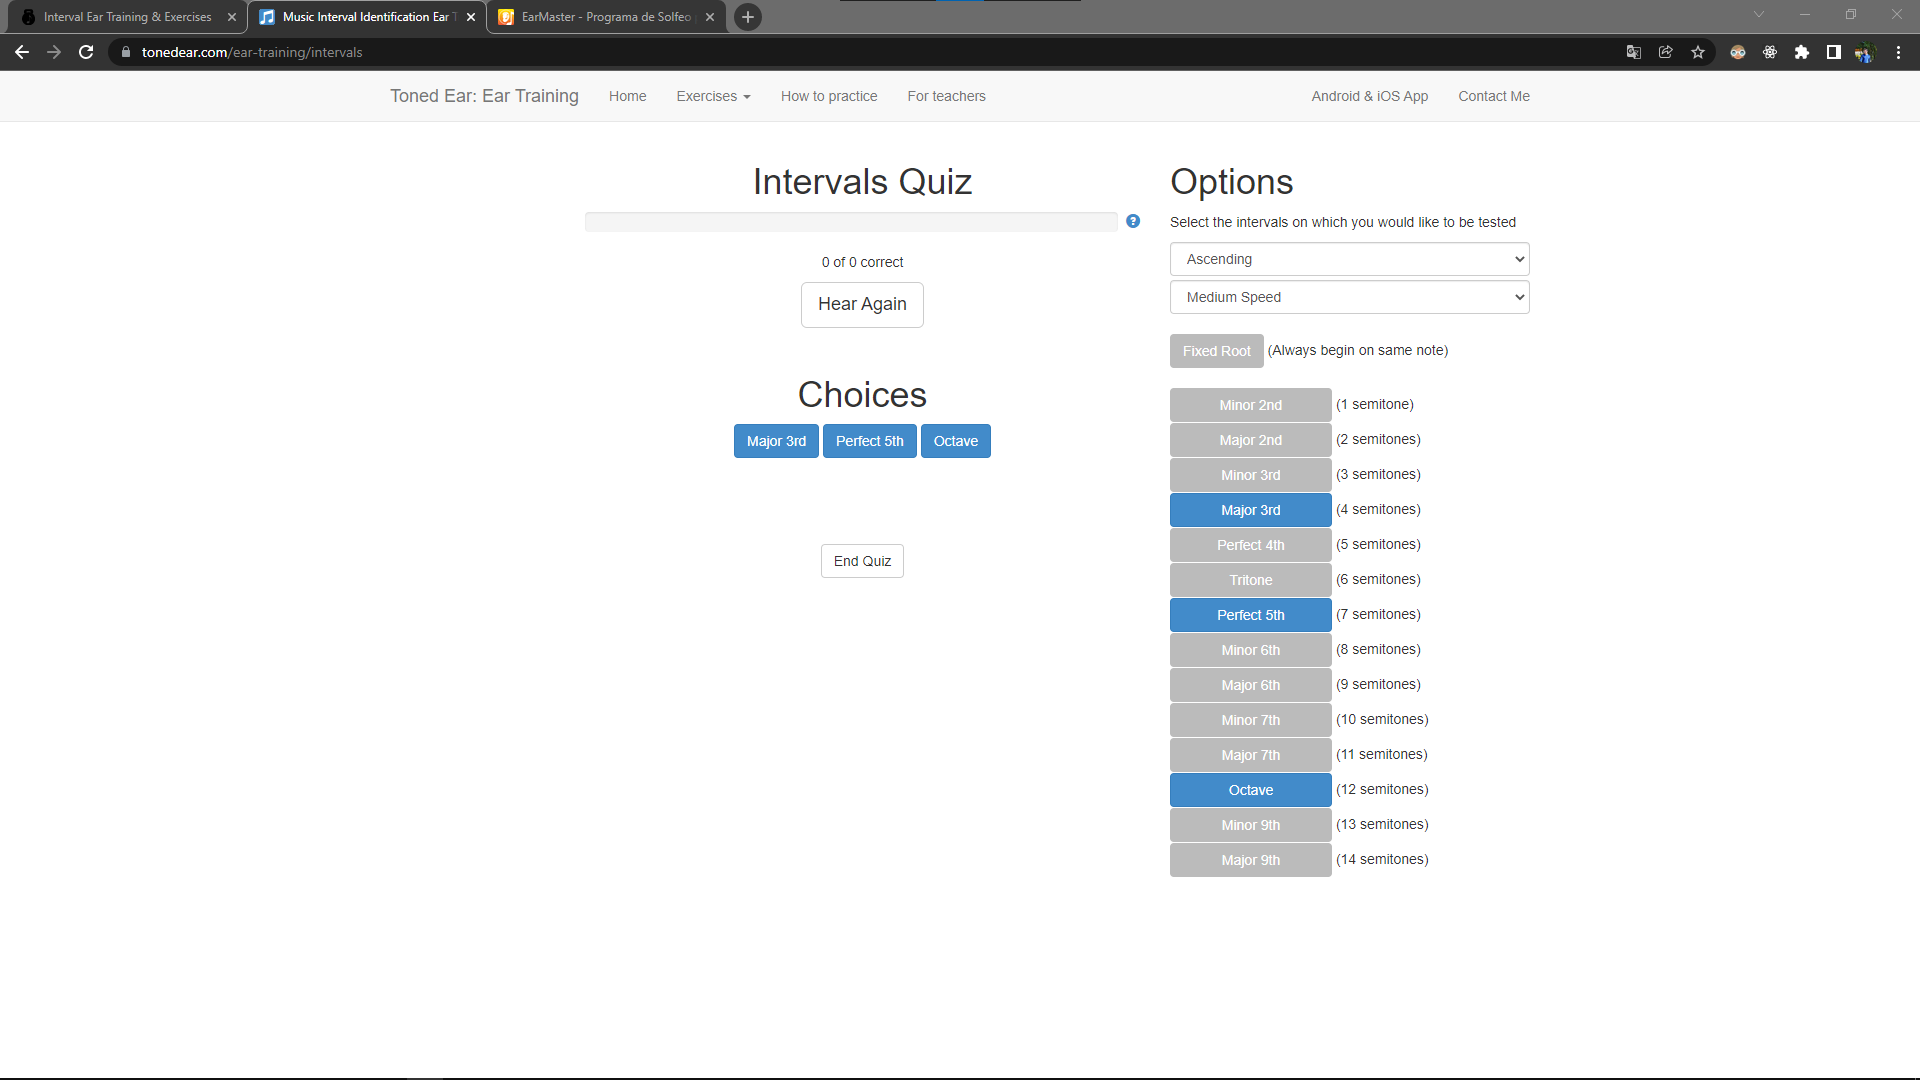
\includegraphics[scale=0.25]{Estado del Arte/tonedear}
    \centering
    \label{fig:tonedear}
    \caption{TonedEar}
\end{figure}

El único fallo encontrado analizando el código la aplicación es que en el ejercicio de identificación de intervalos, no se encuentran todos los intervalos existentes. Podemos observar que siempre una de las dos notas del intervalo será un número MIDI desde 40 hasta 65 y la segunda nota será la primera más un número del 1 al 14 (el atributo interval). Lo que nos da un rango de notas desde 40 hasta 79 cuando el rango de notas MIDI va desde 20 hasta 108 para un piano. Además, este ejercicio no está bien implementado y tiene fallos. Puede ocurrir que la primera nota del intervalo suene después de la segunda como se puede apreciar en las capturas en la función 'playInterval'.

\begin{figure}[H] 
    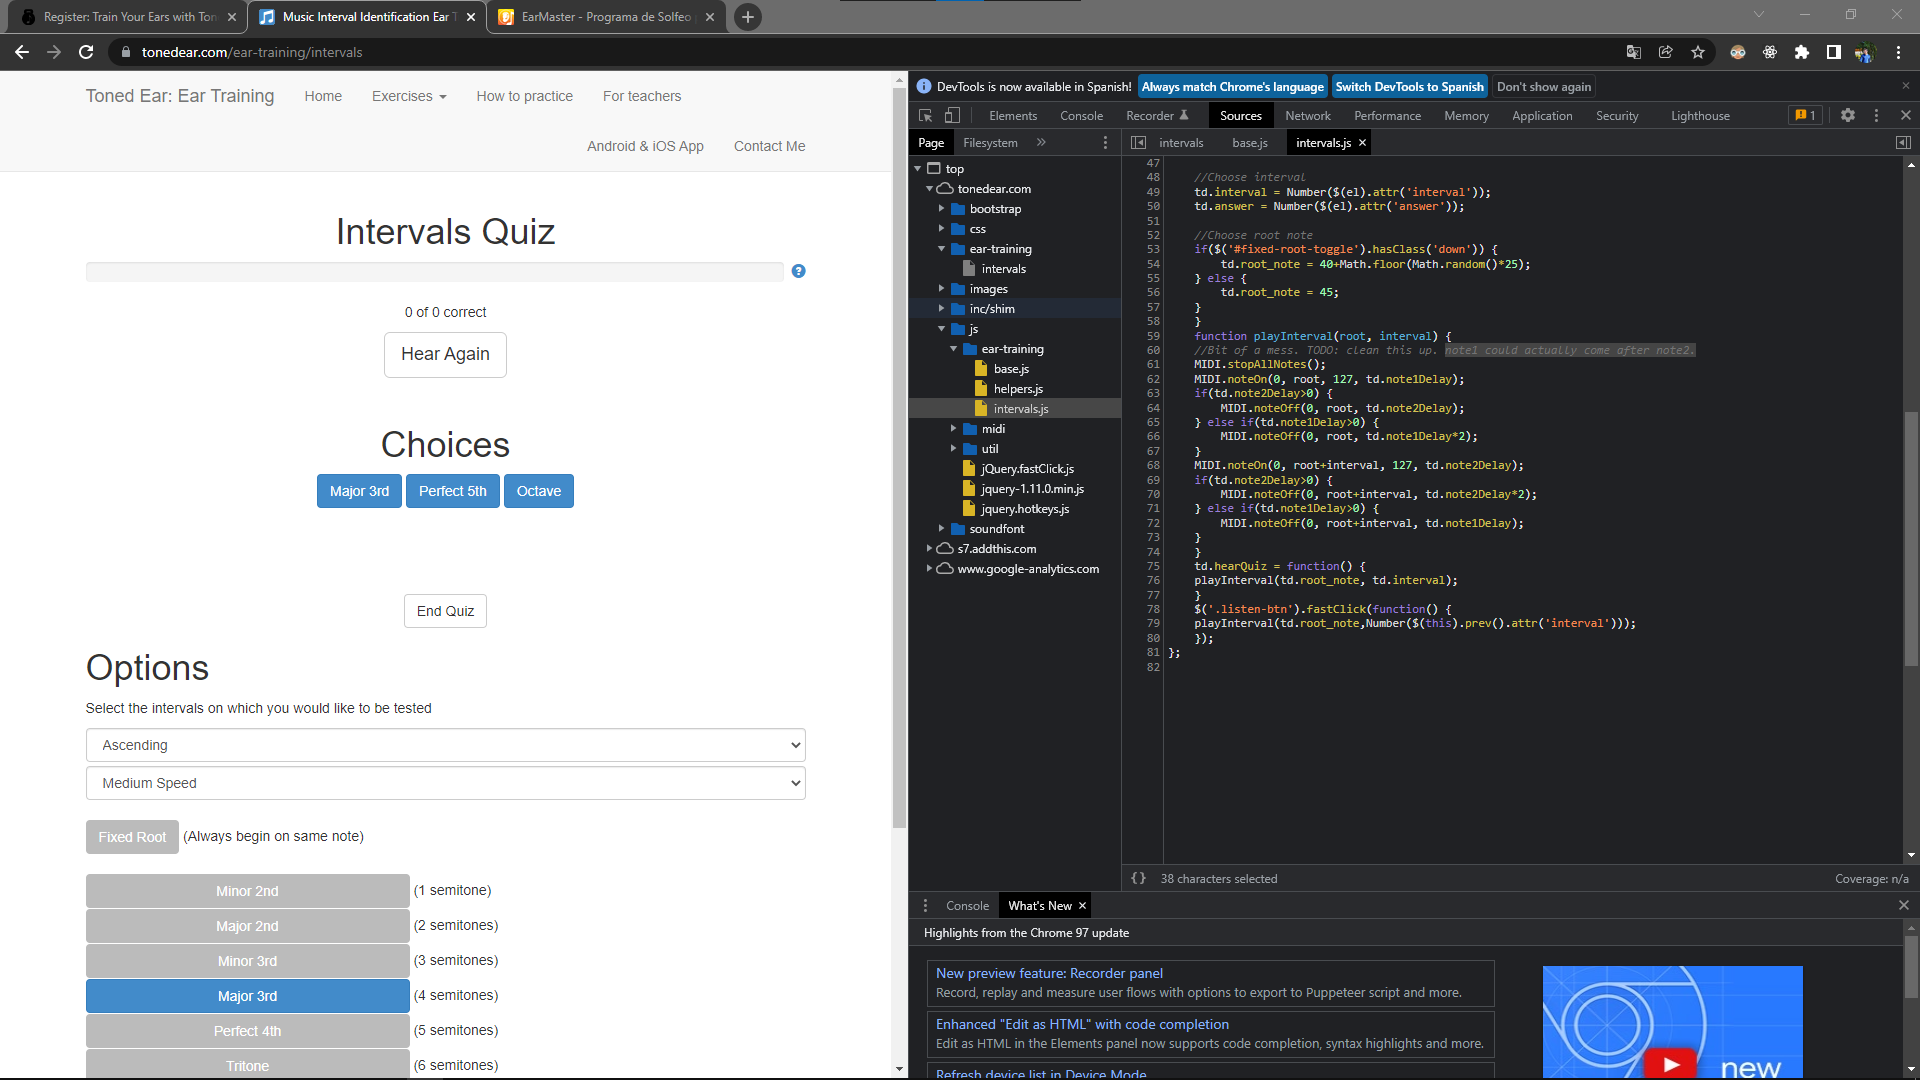
\includegraphics[scale=0.25]{Estado del Arte/tonedearerror}
    \centering
    \label{fig:tonedearerror}
    \caption{TonedEar Error}
\end{figure}

Por último, la aplicación permite personalizar los ejercicios pero no permite cambiar entre instrumentos. El instrumento que suena siempre al pulsar el botón de pregunta es un piano.

\subsection{EarMaster}

Parece ser la más completa y elaborada de todas con más de 2500 ejercicios. Contiene ejercicios para que puedas reconocer, transcribir, leer, cantar y tocar: Intervalos, acordes, progresiones armónicas, escalas, ritmos y melodías.

\begin{figure}[H] 
    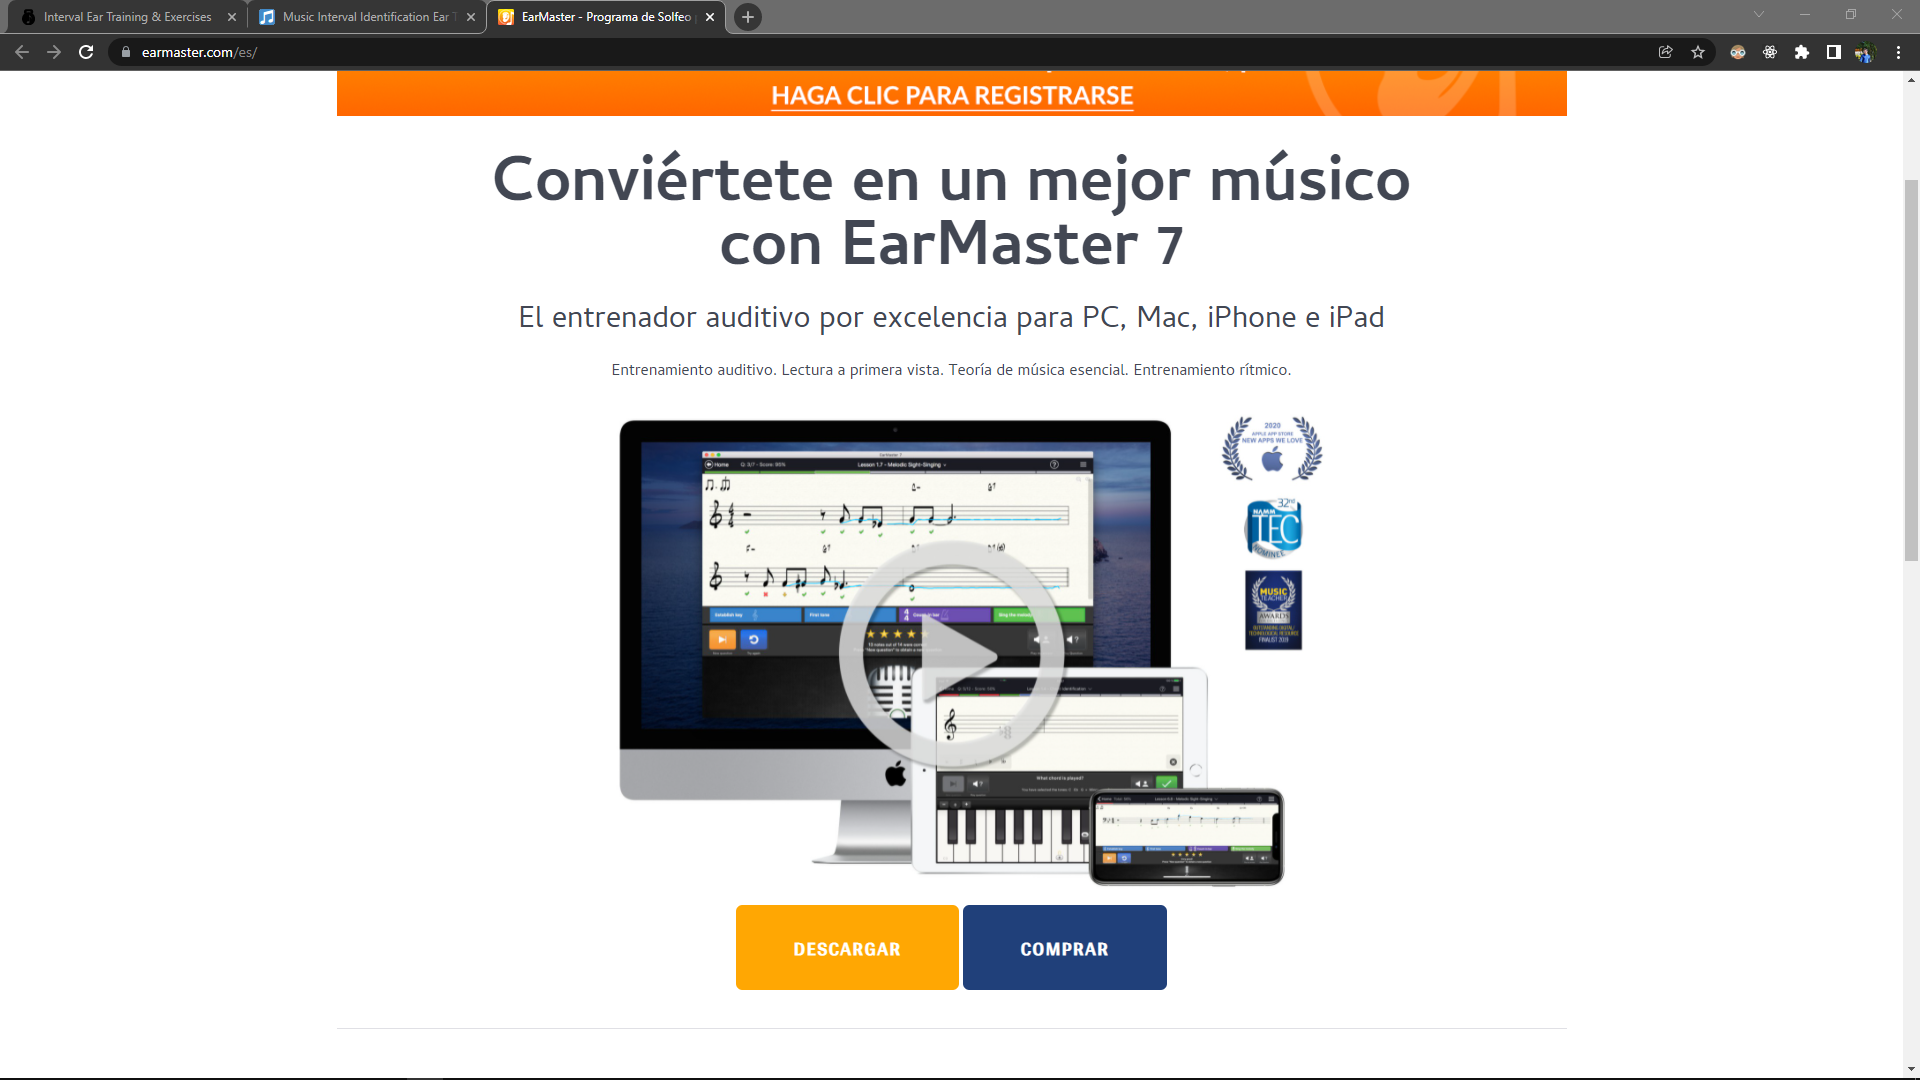
\includegraphics[scale=0.25]{Estado del Arte/earmaster}
    \centering
    \label{fig:earmaster}
    \caption{EarMaster}
\end{figure}

Sin embargo, su contenido gratuito sólo consta de identificación de intervalos y acordes. Para poder hacer uso de la aplicación completa ofrece precios desde los 59,95€ hasta los 99,95€. Aparte, necesitas tener la aplicación instalada para utilizarla, no es una aplicación web. Todo esto resulta en que el usuario al que nos estamos enfocando no pueda usarla. Esta aplicación parece estar más destinada a centros educativos que puedan hacerse cargo de la licencia.

\begin{figure}[H] 
    
\includegraphics[scale=0.5]{Estado del Arte/earmasterprices}
    \centering
    \label{fig:earmasterprices}
    \caption{EarMaster Precios}
\end{figure}

\section{Objetivos}

El objetivo principal del TFG es desarrollar una herramienta que permita ayudar a músicos a desarrollar su oído musical. Mediante el entrenamiento auditivo.

Subobjetivos:
\begin{compactitem}
    \item Desarrollar una interfaz interactiva
    \item Implementar diferentes tipos de ejercicios 
    \item Incluir varios instrumentos
\end{compactitem}

\section{Estructura del documento}

En este apartado se especificará la estructura que plantea este breve trabajo o memoria. El objetivo de dicho punto es acercar al lector las diferentes partes que componen este proyecto, así como ayudarle en la comprensión de este. Se espera que sea lo suficientemente clarificador y que permita una lectura comprensible, rápida y amena del trabajo que nos ocupa.

Este trabajo se centra en el siguiente proceso combinando de Design Thinking, Lean Startup y Metodologías Agile para la creación de un Producto Mínimo Viable. De esta manera conseguimos un proceso que parte de la nada, **se centra** en el usuario, **gestiona** el desarrollo, **integra** el error y es **iterable**.

\begin{figure}[H] 
    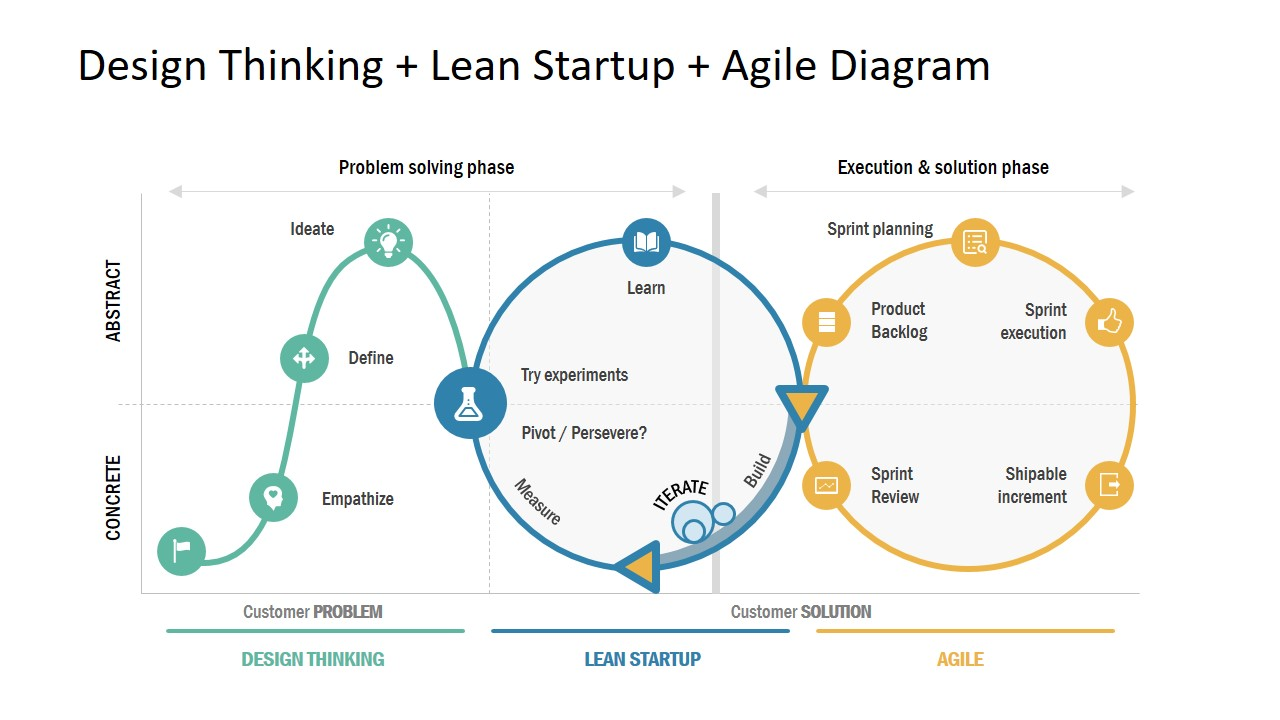
\includegraphics[scale=0.45]{LeanDesignAgile}
    \centering
    \label{fig:Lean Design Agile}
    \caption{Diagrama Design Thinking + Lean Startup + Agile}
\end{figure}

Este proceso se ha dividido en la memoria en los siguientes tres capítulos:

\begin{itemize}
    \item \textbf{Ideación y Diseño:} Este capítulo recoge todo lo relacionado con la fase de ideación y puesta en marcha de la solución. Recoge explicaciones del proceso de Design Thinking y Lean Startup. Aquí se pueden encontrar el diseño y los prototipos de la aplicación.
    \item \textbf{Metodologías Ágiles:} Este capítulo recoge lo relacionado para llevar a cabo la gestión y desarrollo del software utilizando Scrum y prácticas DevOps. Aquí se puede encontrar cómo se ha realizado la gestión, especificación de requisitos, integración continua y despliegue continuo.
    \item \textbf{Descripción Informática:} Este capítulo se centra en lo relacionado con la implementación de la solución. Aquí se puede encontrar las tecnologías usadas, los detalles de implementación del código, buenas prácticas y testing.
\end{itemize}


% \afterpage{\blankpage} % puede generar problema en índice de contenidos
% \newpage


%%%%%%%%%%%%%%%%%%%%%%%%%%%%%% 2 Contenidos Principales %%%%%%%%%%%%%%%%%%%%%%%%%%%

\chapter{Ideación y Diseño}

Para encontrar una solución viable al problema que se plantea y qué aporte un valor real a los usuarios, necesitamos de algún método que nos permita diseñar una solución de manera efectiva bajo unas condiciones de incertidumbre extrema.

Para crear esta propuesta de valor, se puede utilizar Design Thinking como método de generación de ideas innovadoras y Lean Startup como método de aprendizaje validado.

\section{Design Thinking}

Es un método para generar ideas innovadoras que centra su eficacia en entender y dar solución a las necesidades reales de los usuarios. Proviene de la forma en la que trabajan los diseñadores de producto. De ahí su nombre, que en español se traduce de forma literal como "Pensamiento de Diseño" o "La forma en la que piensan los diseñadores".

Mientras que Lean startup surge como una metodología que permite impactar en el mercado con éxito, el Design Thinking busca el diseño de experiencias de alto valor, centradas en el usuario.

Dado que Lean Startup no se centra en el usuario, lo ideal es coger lo mejor de ambas metodologías. Añadir esta metodología al proceso de creación ayuda a conocer al cliente en profundidad y encontrar soluciones prácticas ante sus problemas en un proceso ágil.

\subsection{Etapas}

El proceso de Design Thinking se compone de cinco etapas. No es lineal. En cualquier momento se puede ir hacia atrás o hacia delante si se cree oportuno, saltando incluso a etapas no consecutivas. A lo largo del proceso se irá afinando ese contenido hasta desembocar en una solución que cumpla con los objetivos. 

\begin{figure}[H] 
    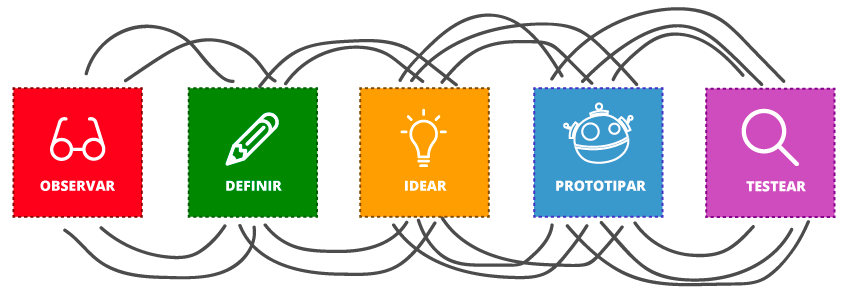
\includegraphics[scale=0.44]{Design Thinking/Etapas}
    \centering
    \label{fig:Design Thinking}
\end{figure}

\subsubsection{Empatizar}

Se realizaron entrevistas al usuario y un estudio profundo de teoría musical para entender al usuario y sus necesidades. Como se explica en el anexo.

\subsubsection{Definir}

La idea parte de la necesidad de músicos amateur que quieren mejorar su nivel de percepción de la música. Sin los medios adecuados resulta imposible llevar a cabo el entrenamiento auditivo que es una parte fundamental para llevar a cabo su propósito. 

\subsubsection{Idear}

Para idear una solución que aporte valor realizamos este MindMap donde nos enfocamos en los principales problemas del usuario y sus posibles soluciones.

\begin{figure}[H]
    \centering
    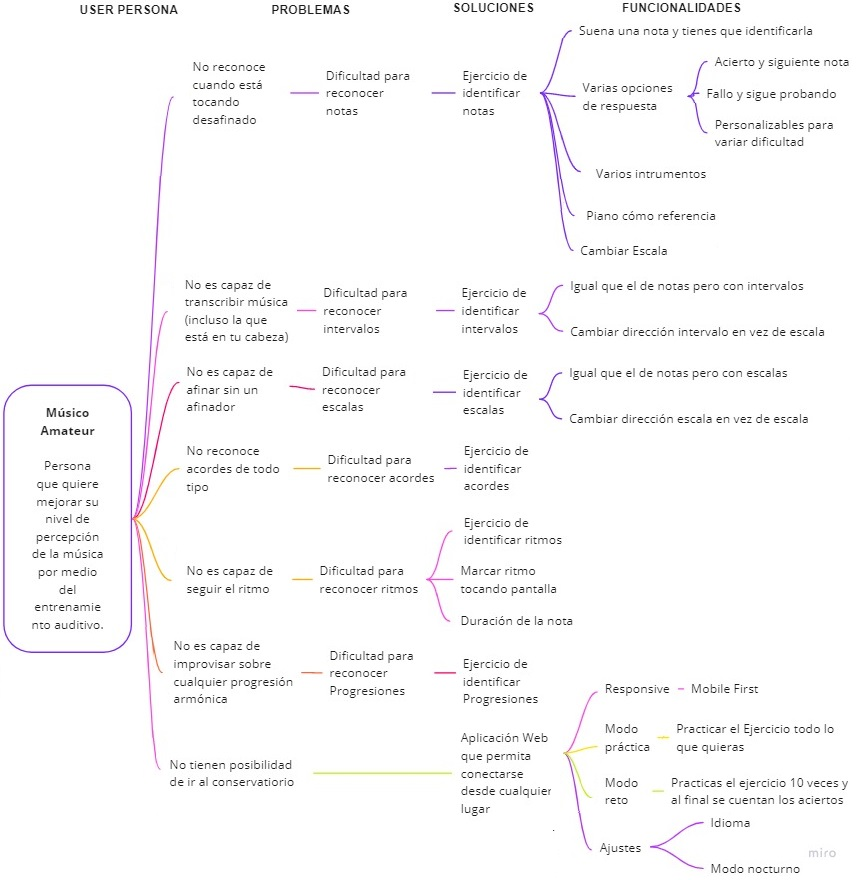
\includegraphics[scale=0.47]{Design Thinking/MindMap}
    \label{fig:Mindmap}
    \caption{MindMap}
\end{figure}

Concluimos que una posible forma de solucionar estos problemas es mediante una Aplicación Web con ejercicios de Entrenamiento Auditivo. 


\subsubsection{Prototipar}

Utilizamos la técnica MoSCoW para establecer las prioridades del proyecto. Teniendo en cuenta nuestras limitaciones: poco tiempo para desarrollar, aprender conceptos musicales y nuevas tecnologías. 

\begin{figure}[H]
    \centering
    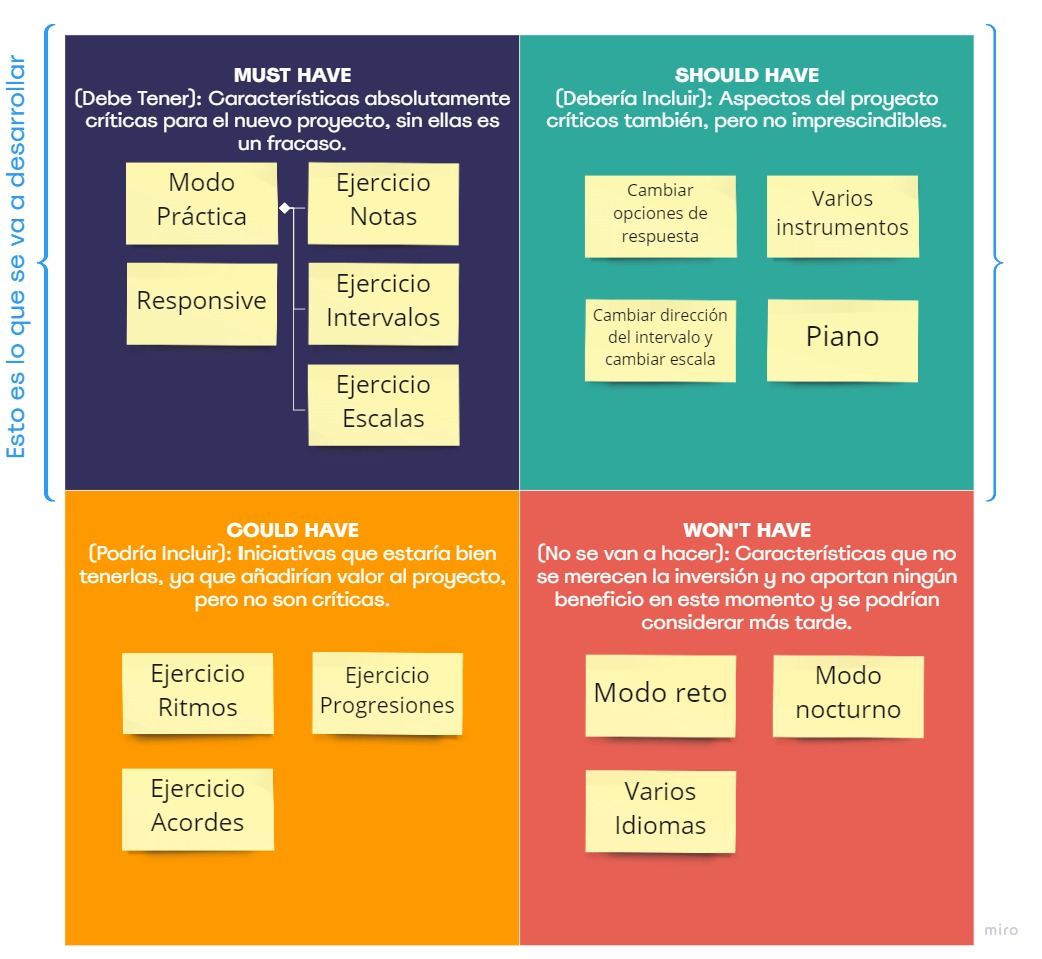
\includegraphics[scale=0.35]{Design Thinking/MosCow}
    \label{fig:MoSCoW}
    \caption{MoSCoW}
\end{figure}

Para crear nuestro producto mínimo viable nos centramos en desarrollar lo que debe tener (must have) y más tarde lo que debería incluir (should have).

Utilizamos la técnica MoSCoW para establecer las prioridades del proyecto. Teniendo en cuenta nuestras limitaciones: poco tiempo para desarrollar, aprender conceptos musicales y nuevas tecnologías. ¿Cuál es el producto mínimo viable (MVP) que puedo crear para obtener resultados?

Una vez establecidas las prioridades del proyecto pasamos a visualizarlas diseñando el Prototipo teniendo en cuenta la filosofía de diseño Mobile First.

    \begin{figure}[H]
        \centering
        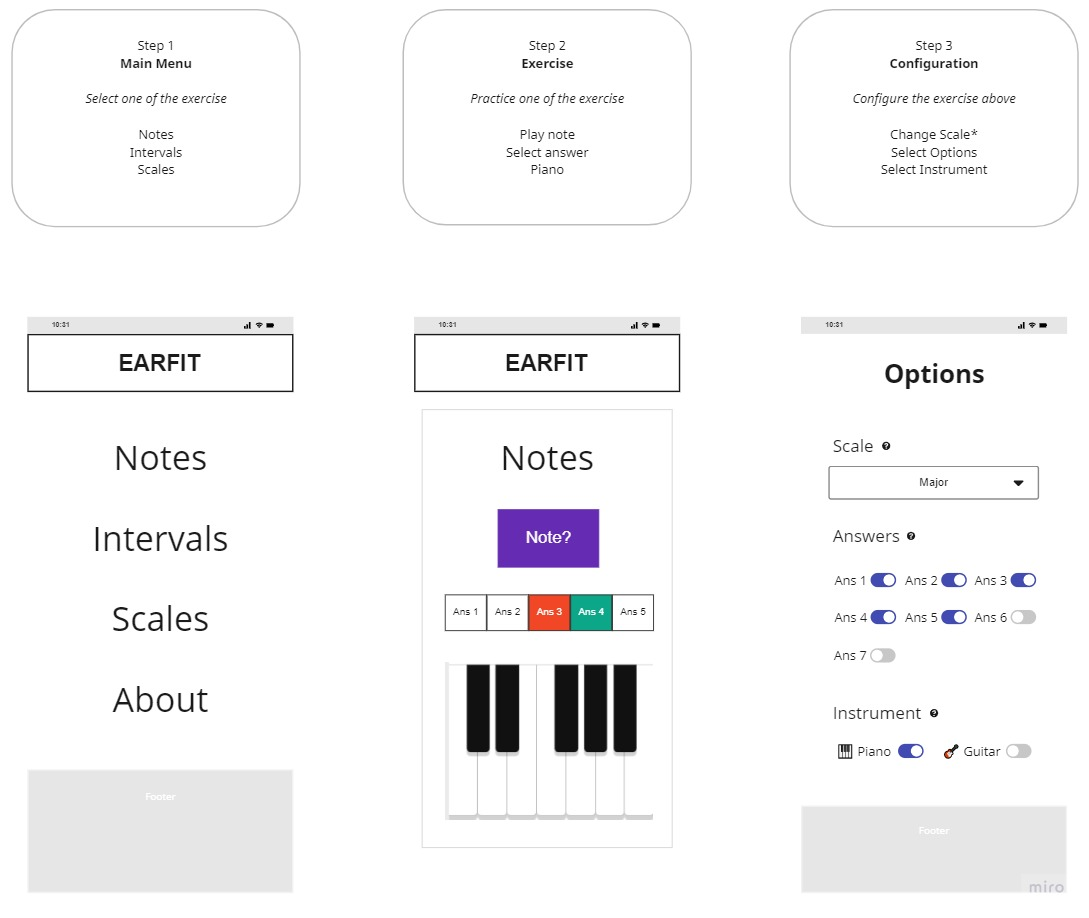
\includegraphics[scale=0.33]{Design Thinking/Prototipo/Small/Prototipo}
        \label{fig:PrototipoSmall}
        \caption{Prototipo Pantallas Pequeñas}
    \end{figure}

    \begin{figure}[H]
        \centering
        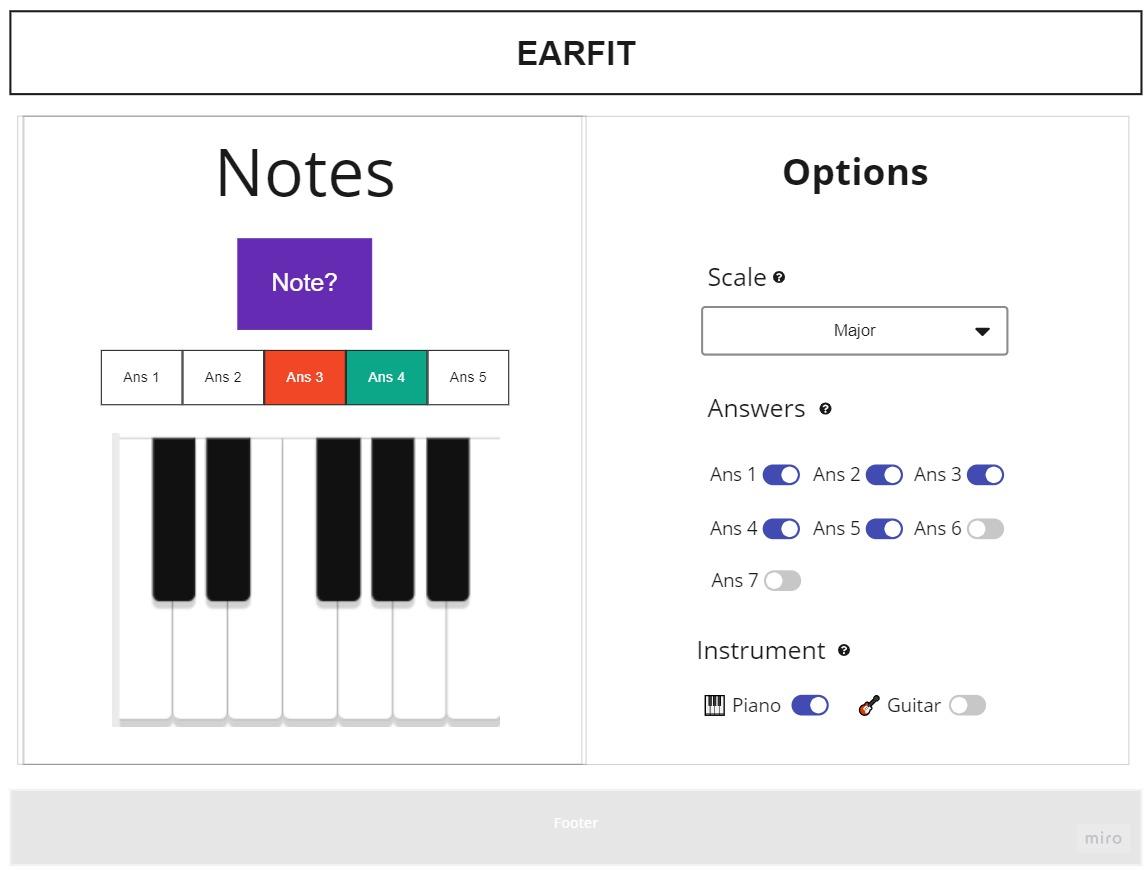
\includegraphics[scale=0.3]{Design Thinking/Prototipo/Medium/Notes}
        \label{fig:PrototipoMedium}
        \caption{Prototipo Pantallas Medianas}
    \end{figure}
    
    \begin{figure}[H]
        \centering
        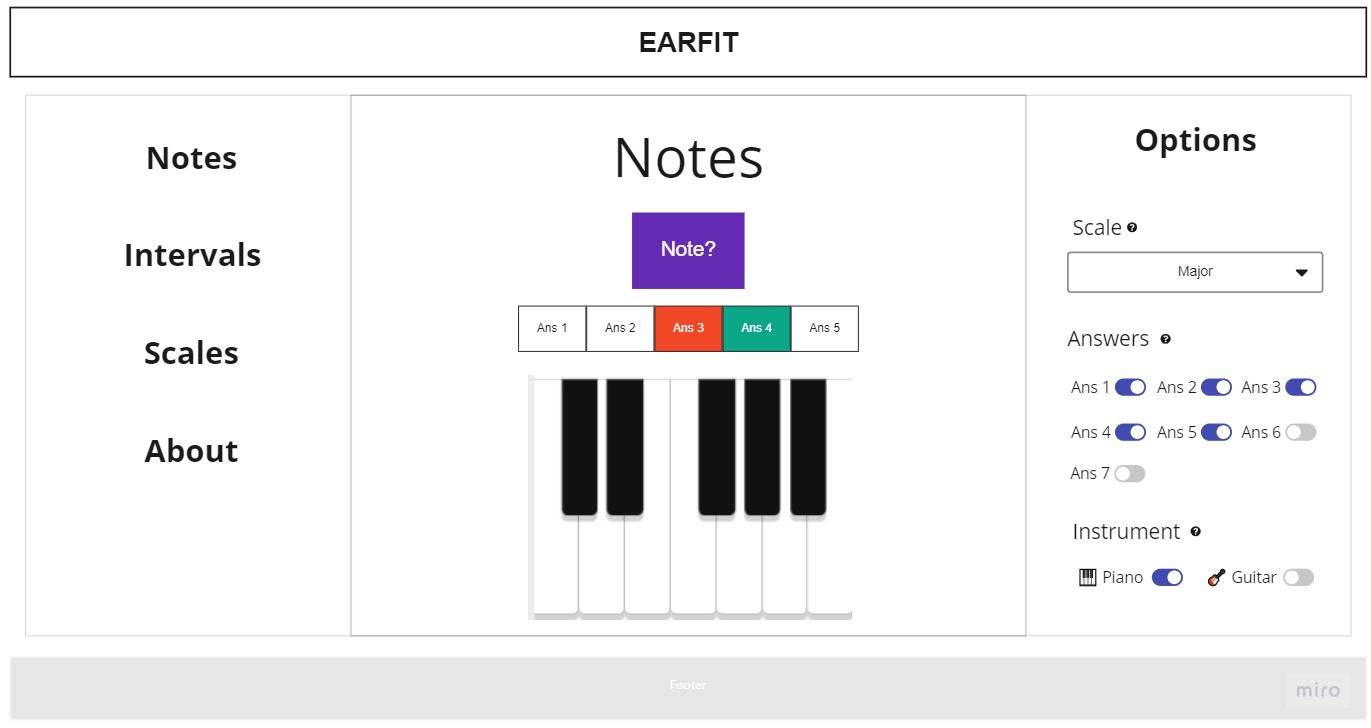
\includegraphics[scale=0.28]{Design Thinking/Prototipo/Large/Notes}
        \label{fig:PrototipoLarge}
        \caption{Prototipo Pantallas Grandes}
    \end{figure}

La ventaja principal del uso de prototipos en UX o Experiencia de Usuario es que, ayudan a plasmar visualmente los objetivos y como se alinean con las expectativas y necesidades de los usuarios y si son satisfechas a través del producto diseñado.

Modificar un prototipo, tiene un coste menor que modificar el producto digital, por lo que supone también una ventaja en el ahorro de costes dentro del proceso de desarrollo.

Ayuda a que el cliente ya tenga una visión sobre parte del proyecto y que nos pueda proporcionar su feedback desde las fases tempranas.

\subsubsection{Testear}

Después de haber testeado los primeros diseños con el usuario, haber hecho correcciones y haber validado el último prototipo que hemos visto anteriormente, pasamos a crear la solución aplicando el método Lean Startup.

\section{Lean Startup}

Es un método riguroso para agilizar la puesta en marcha de soluciones y optimizarlas con base en un proceso de aprendizaje y de corrección iterativa. Comenzó con el método de desarrollo de clientes y el método Lean en los sistemas de fabricación japoneses popularizado por Toyota.

La metodología Lean Startup se basa en el Circuito de feedback de información: crear, medir, aprender. Crear una hipótesis, diseñar un experimento (Producto Mínimo Viable) para testear esa hipótesis, llevar a cabo el experimento, reunir datos, reflexionar y ver si validan o rechazan la hipótesis para pivotar.

\begin{figure}[H]
    \centering
    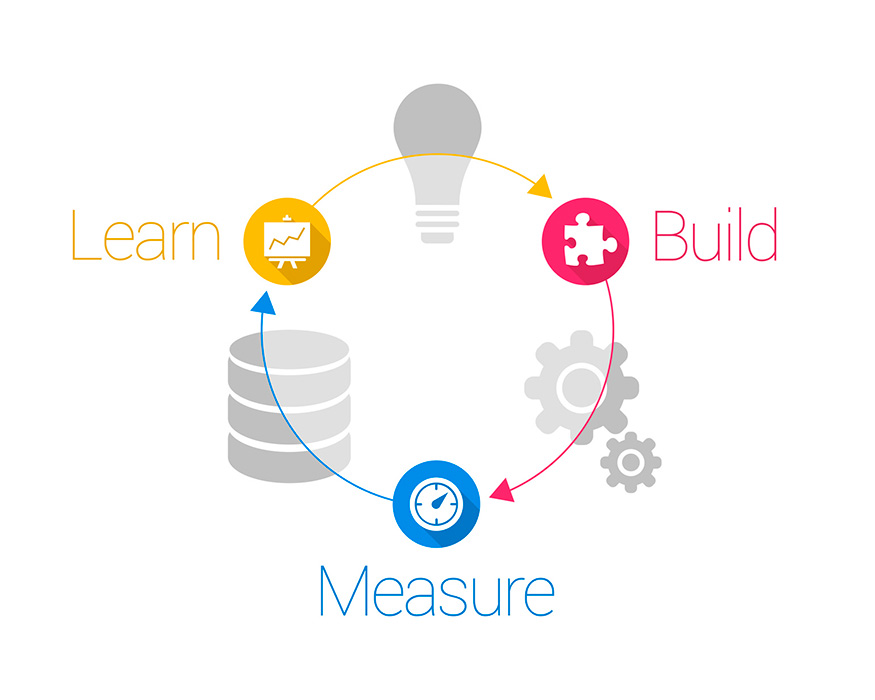
\includegraphics[scale=0.3]{Lean Startup/CircuitoFeedback}
    \label{fig:LeanStartup}
    \caption{Lean Startup}
\end{figure}

El Lean Startup sirve para acortar los ciclos de desarrollo, medir el progreso y ganar feedback por parte de los usuarios. Esto se consigue porque se basa en el aprendizaje validado, la experimentación científica y la iteración en los lanzamientos del producto. 

Aunque por su nombre pueda parecer que sólo esta enfocado al mundo Startup y crear una nueva empresa, en realidad es una herramienta imprescindible para la puesta en marcha de soluciones software. Por eso, hemos decidido usar este método para crear nuestra solución.

Por ahora, sólo saber que se ha seguido este proceso de crear, medir, aprender. Y que los diseños, los requisitos y la aplicación han ido adoptando cambios según el desarrollo. Para la fase de creación se utilizaron Metodologías Ágiles y para no alargar mucho este trabajo las partes de medir y aprender, donde aparecen cosas cómo la técnica del Conserje, métricas de engagement, tiempo en el producto, retención, referencia, Test A/B y lecciones aprendidas para pivotar; se explicarán en el anexo junto con una explicación más detallada de todo el proceso. 
(revisar)

\chapter{Metodologías Ágiles}

Para llevar a cabo la idea de manera exitosa necesitamos asegurar un proceso visible, controlado, repetitivo, eficiente y predecible. Necesitamos adaptar las formas de trabajo a las necesidades del proyecto, prolongando respuestas rápidas y flexibles para acomodar el desarrollo.

La agilidad es la habilidad, que facilita la adaptación, de manera rápida y efectiva en circunstancias cambiantes, para garantizar la entrega de valor continuo, en ciclos cortos de tiempo y con el mínimo coste.

Para ser ágiles mientras desarrollamos podemos beneficiarnos de DevOps, como filosofía de desarrollo y Scrum, como modelo organizativo.

\section{Scrum}

Scrum es un proceso de gestión que reduce la complejidad en el desarrollo de productos para satisfacer las necesidades de los clientes. Se considera un marco de gestión de proyectos ágil.

Con Scrum, un producto se basa en una serie de iteraciones llamadas sprints que dividen proyectos grandes y complejos en porciones minúsculas. Priorizadas por el beneficio que aportan al receptor del producto.

\begin{enumerate}
    \item Un Product Owner ordena el trabajo de un problema complejo en un Product Backlog.
    \item El Equipo Scrum convierte una selección del trabajo en un Incremento de valor durante un Sprint.
    \item El Equipo Scrum y sus partes interesadas inspeccionan los resultados y se ajustan para el próximo Sprint.
    \item *Repetir*
\end{enumerate}

Scrum no es un proceso o una técnica para desarrollar/construir productos, realmente es un marco de trabajo donde podemos emplear un conjunto de diferentes procesos y técnicas, siendo muy fácil de implantar y muy popular en el desarrollo software por los resultados rápidos que consigue.

\begin{figure}[H]
    \centering
    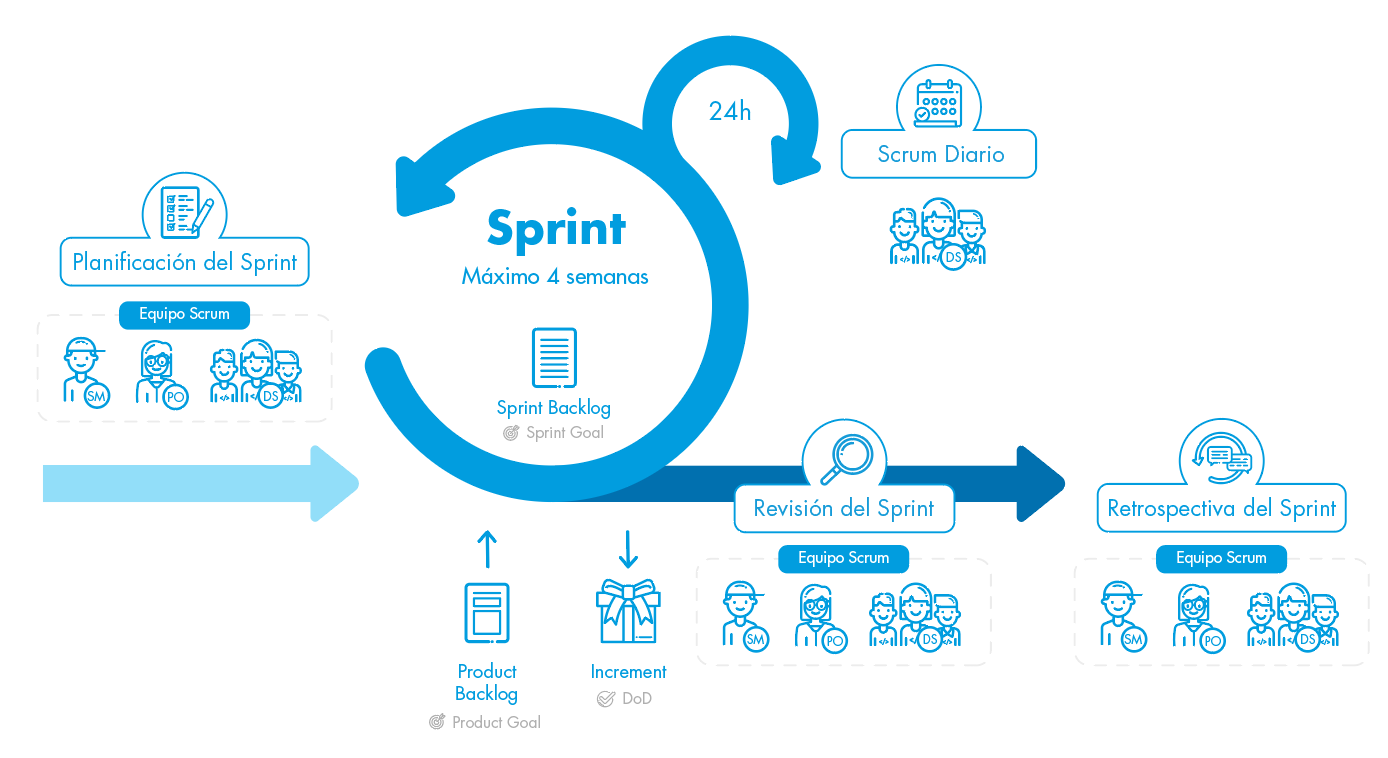
\includegraphics[scale=0.39]{Scrum/Scrum}
    \label{fig:Scrum}
    \caption{Scrum}
\end{figure}

Implementar este marco de trabajo nos permite obtener resultados pronto, reduciendo el Time to Market, es decir, a tener lo antes posible en el mercado nuestro producto o una característica de nuestro producto, aumentando la satisfacción del cliente. Donde los requisitos son cambiantes o poco definidos, aportando tolerancia al cambio.

Es ideal para crear nuevos productos poniendo el foco en el cliente y detectar fallos pronto. Lo que se traduce en una mayor calidad del producto, reducción de costes y optimización del riesgo.

\subsection{User Story Map}

Es un método de mapeo de UX (experiencia de usuario) que se utiliza para delinear las interacciones que se espera que realicen los usuarios para completar sus objetivos en un producto digital. Ayuda a definir el viaje o casos de uso del usuario en el producto.

\begin{figure}[H]
    \centering
    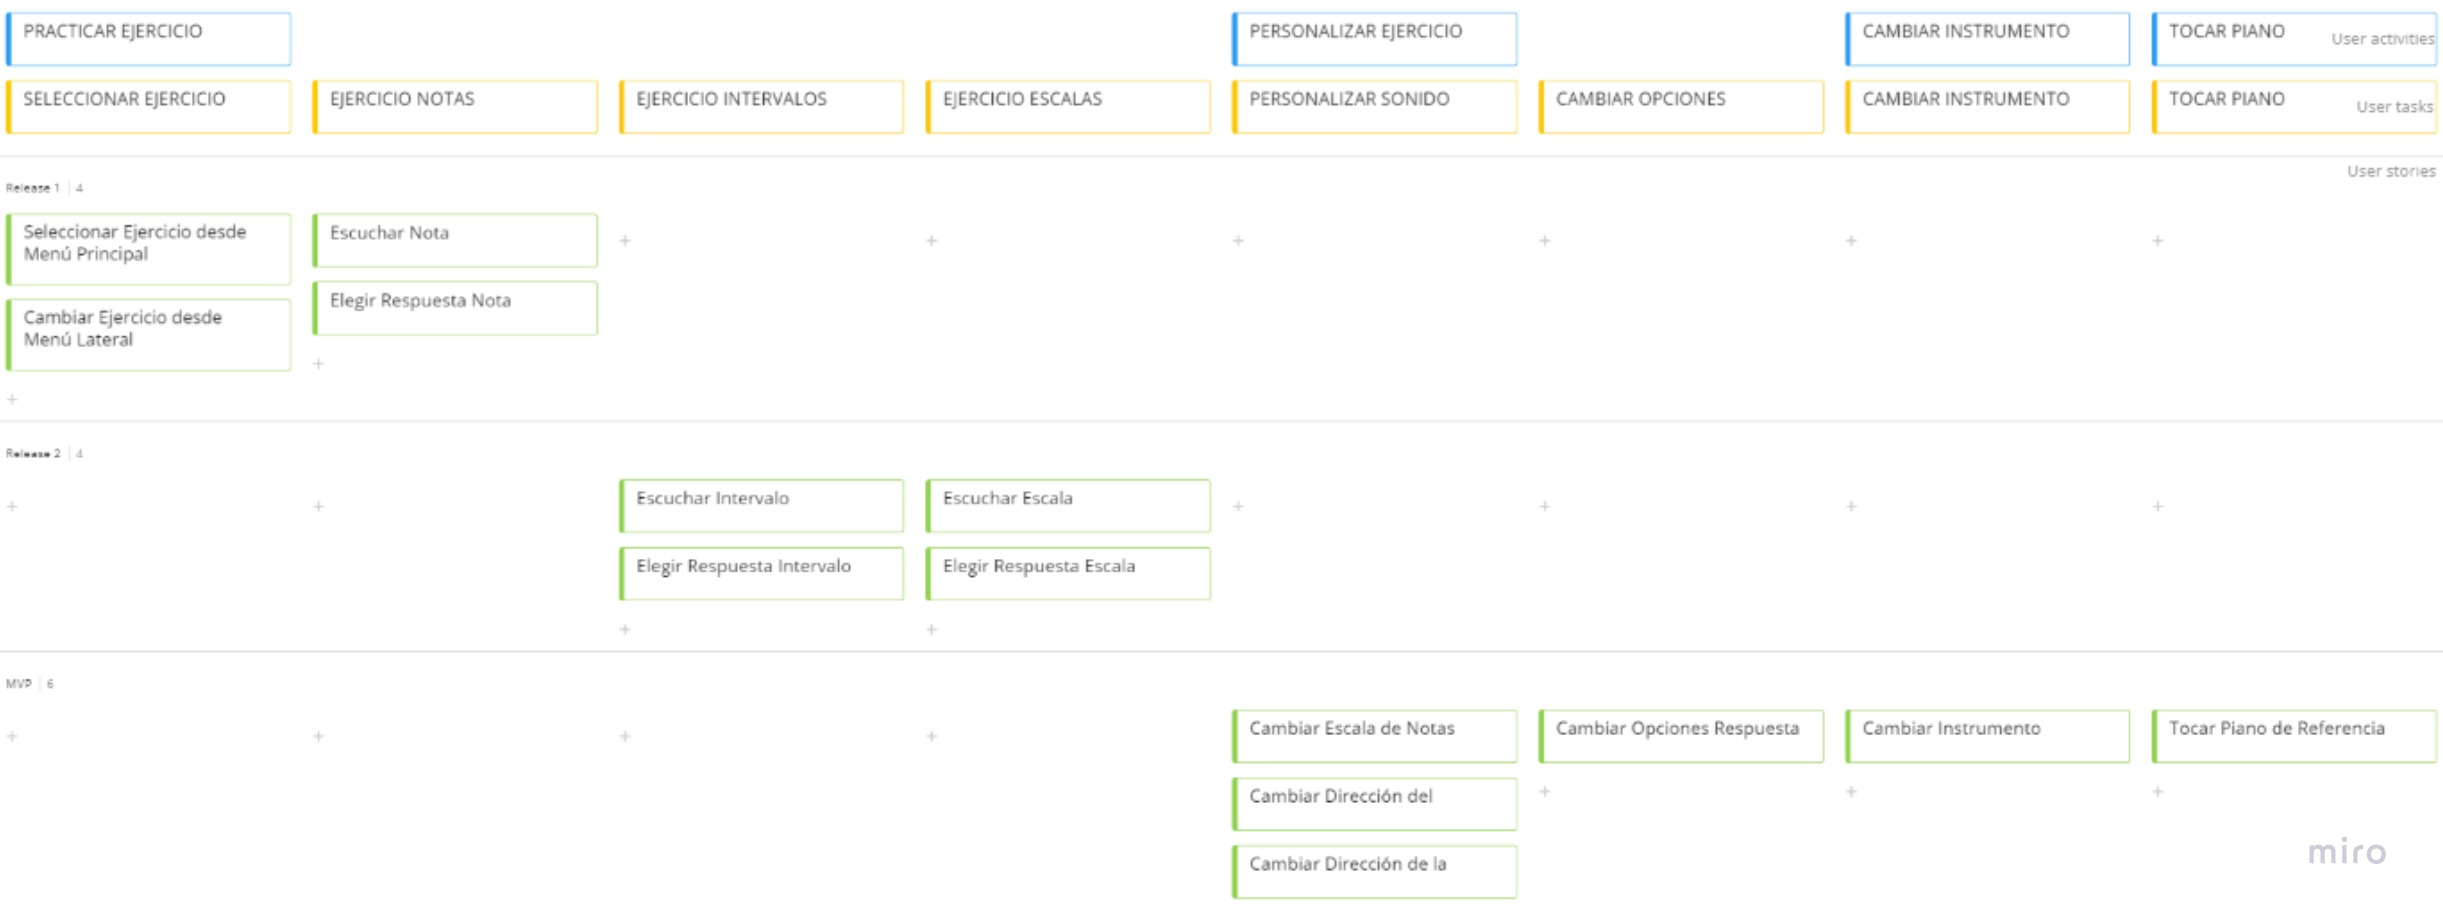
\includegraphics[scale=0.25]{Scrum/UserStoryMap}
    \label{fig:UserStoryMap}
    \caption{User Story Map}
\end{figure}

\subsection{Scrum Board}

Para visualizar el trabajo utilizamos un Scrum Board. Esto nos permite separar en pequeñas tareas cada historia de usuario y minimizar los riesgos de entrega. Realizando una construcción iterativa incremental donde se integra al final de cada sprint para validar el resultado. 

\begin{figure}[H]
    \centering
    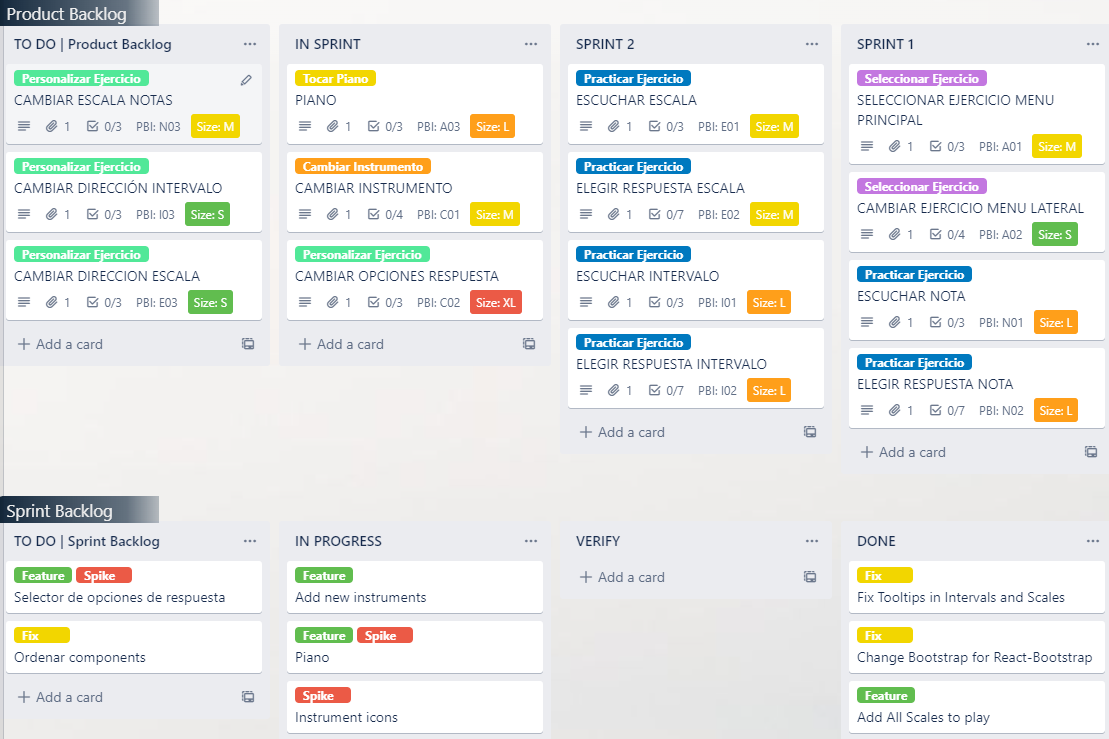
\includegraphics[scale=0.47]{Scrum/ScrumBoard}
    \label{fig:ScrumBoard}
    \caption{Scrum Board}
\end{figure}

\subsection{User Stories}

Las historias de usuarios son descripciones breves y sencillas de las características o requisitos del sistema contadas desde la perspectiva de un usuario o cliente del sistema. Estas historias se dividen en tareas más pequeñas que ir completando hasta cumplir con los criterios de aceptación. Cada historia de usuario es un incremento en el valor del producto.

\begin{figure}[H]
    \centering
    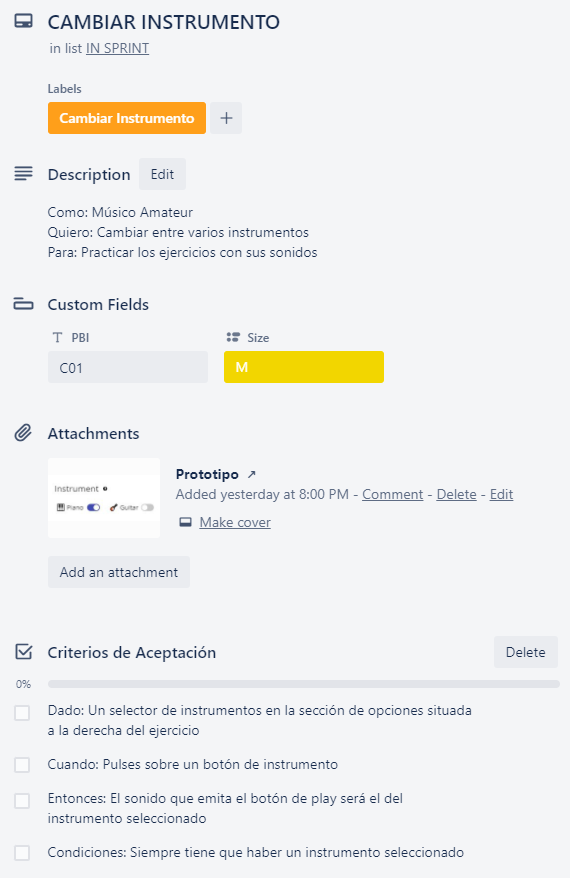
\includegraphics[scale=0.7]{Scrum/UserStory}
    \label{fig:UserStory}
    \caption{User Story}
\end{figure}

\section{DevOps}

El término DevOps, que es una combinación de los términos ingleses development (desarrollo) y operations (operaciones), designa la unión de personas, procesos y tecnología para ofrecer valor a los clientes de forma constante.

DevOps describe los enfoques para agilizar los procesos con los que una idea (como una nueva función de software, una solicitud de mejora o una corrección de errores) pasa del desarrollo a la implementación, en un entorno de producción en que puede generar valor para el usuario.

La creación de registros de trabajo pendiente, el seguimiento de los errores, la administración del desarrollo de software ágil con Scrum, el uso de paneles Kanban y la visualización del progreso son algunas de las formas en las que los equipos de DevOps planean con agilidad y visibilidad.

El desarrollo de aplicaciones modernas requiere procesos diferentes a los enfoques del pasado. Las nuevas empresas utilizan enfoques ágiles para desarrollar sistemas de software.

\begin{figure}[H]
    \centering
    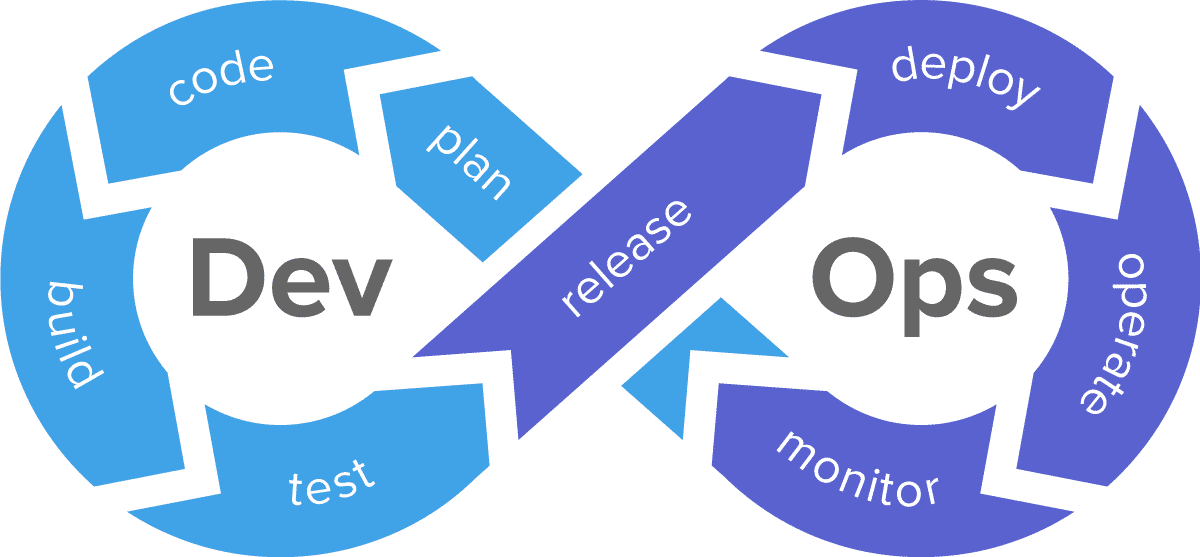
\includegraphics[scale=0.24]{DevOps/DevOps}
    \label{fig:DevOps}
    \caption{DevOps}
\end{figure}

DevOps permite fabricar software más rápidamente, con mayor calidad, menor coste y una altísima frecuencia de releases. Al adoptar prácticas de DevOps, se asegura la confiabilidad, la alta disponibilidad y el objetivo de ningún tiempo de inactividad del sistema.

El primero de los 12 principios del Manifiesto Ágil es el siguiente: "Satisfacer a los clientes mediante la distribución de software continua y oportuna". Este es el motivo por el que es importante aplicar prácticas de DevOps, cómo la integración continua y el despliegue continuo.

\subsection{Integración Continua (CI)}

La integración continua es una práctica de DevOps mediante la cual los desarrolladores combinan los cambios en el código en un repositorio central de forma periódica. Para implantar integración continua solemos definir un “pipeline”, un conjunto de etapas, de fases por las que va pasando el software y que se automatizan. 

En nuestro caso usamos Github, que es un servicio basado en la nube, cómo herramienta de control de versiones Git. Y utilizamos Gitflow, que es un modelo alternativo de creación de ramas en Git en el que se utilizan ramas de función y varias ramas principales.

\begin{figure}[H]
    \centering
    \includegraphics[scale=0.58]{DevOps/Gitflow}
    \label{fig:Gitflow}
    \caption{Gitflow}
\end{figure}

Su funcionamiento se basa en dos ramas principales: la rama de producción y la rama de desarrollo. De la rama de desarrollo se van sacando nuevas ramas de funcionalidades y uniendo a está a medida que se completan. Un vez una nueva versión está lista se une la rama de desarrollo con la de producción generando una nueva release.

\subsection{Despliegue Continuo (CD)}

El despliegue continuo es una estrategia de DevOps en la que los cambios de código de una aplicación se publican automáticamente.

Para entregar funcionalidades de software de forma frecuente a través de la automatización de despliegues utilizamos GitHub Actions el cuál nos permite automatizar, personalizar y ejecutar estos flujos de trabajo directamente desde nuestro repositorio.

El flujo consistía en que cada vez que se actualizaba el repositorio mediante una subida de código, éste automáticamente desplegaba las nuevas actualizaciones en Vercel, que es una plataforma en la nube que permite a los desarrolladores alojar sitios web y servicios web que escalan automáticamente y no requieren supervisión.

\begin{figure}[H]
    \centering
    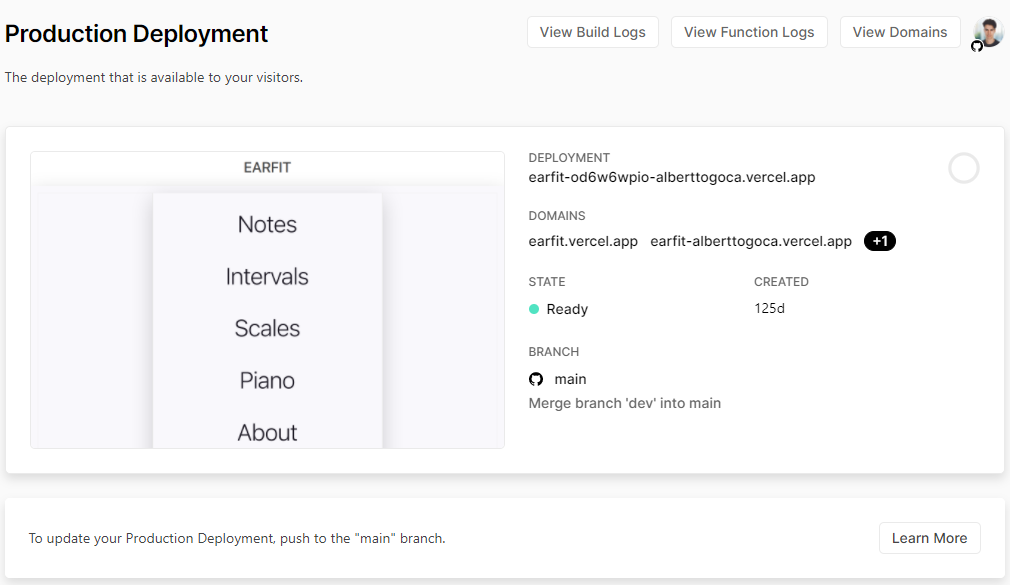
\includegraphics[scale=0.54]{DevOps/Vercel}
    \label{fig:Vercel}
    \caption{Vercel}
\end{figure}

\chapter{Descripción Informática}

Para desarrollar una aplicación de calidad es necesario el uso de unas guías de estándares de calidad de código y un moderno stack tecnológico. A continuación se encuentra una detallada descripción informática incluyendo tecnologías, diseño, implementación y pruebas.

\section{Stack Tecnológico}

Después de una larga investigación y comparación de tecnologías teniendo en mente las necesidades del proyecto. Se llegó a la conclusión de que estás herramientas, frameworks y lenguajes eran los necesarios para implementar esta aplicación. Es necesario explicar cómo funcionan estas tecnologías para entender más tarde la arquitectura y el código de la aplicación.

Otras herramientas no relacionadas con la implementación en sí fueron: Miro, Notion, Trello.

\subsection{Next.js}

Creado por Vercel, Next.js es un framework de trabajo creado sobre Node.js y basado en React que permite crear Single-page Applications (SPA) y aplicaciones web de alto rendimiento a través de la renderización del lado del servidor (Server-side Rendering).

Next nos permite, instalando una sola dependencia, tener configurado todo lo que necesitamos para crear una aplicación de **React** usando Babel y Webpack.  Estas son las características que nos ofrece sin apenas tener que configurarlo:

\begin{itemize}
    \item Un **sistema de enrutamiento** intuitivo **basado en páginas** con soporte para rutas dinámicas: En Next.js, una página es un componente de React exportado desde un archivo .js, .jsx, .ts o .tsx en el directorio de "pages". Cada página está asociada con una ruta basada en su nombre de archivo.
    \begin{figure}[H]
        \centering
        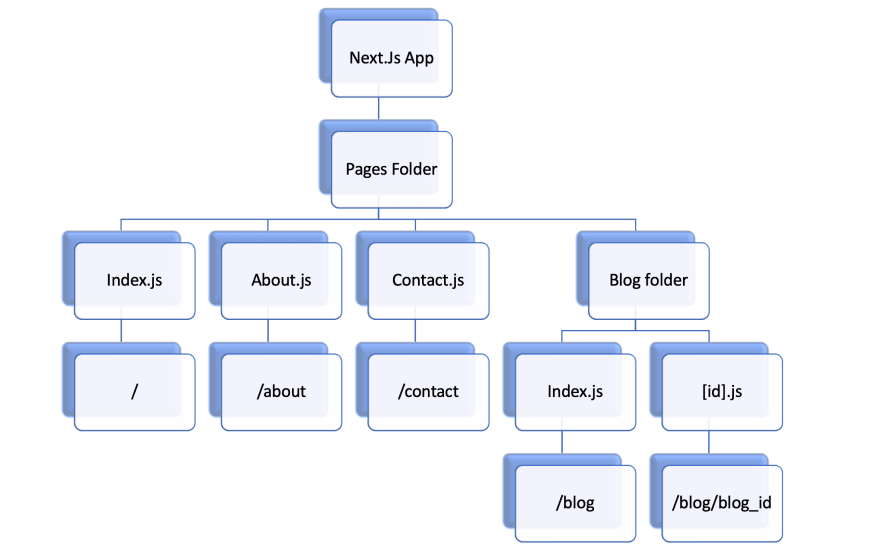
\includegraphics[scale=0.4]{Nextjs/Routing}
        \label{fig:nextjs_routing}
        \caption{Nextjs Routing}
    \end{figure}
    
    \item **Pre-rendering**: De forma predeterminada, Next.js procesa previamente cada página. Esto significa que genera HTML para cada página por adelantado, en lugar de que JavaScript del lado del cliente lo haga todo (Ver figuras 1, 2 y 3). 
    \begin{figure}[H]
        \centering
         \subfloat[Sin Pre-rendering]{
          \label{f:nextjs_noprerendering}
           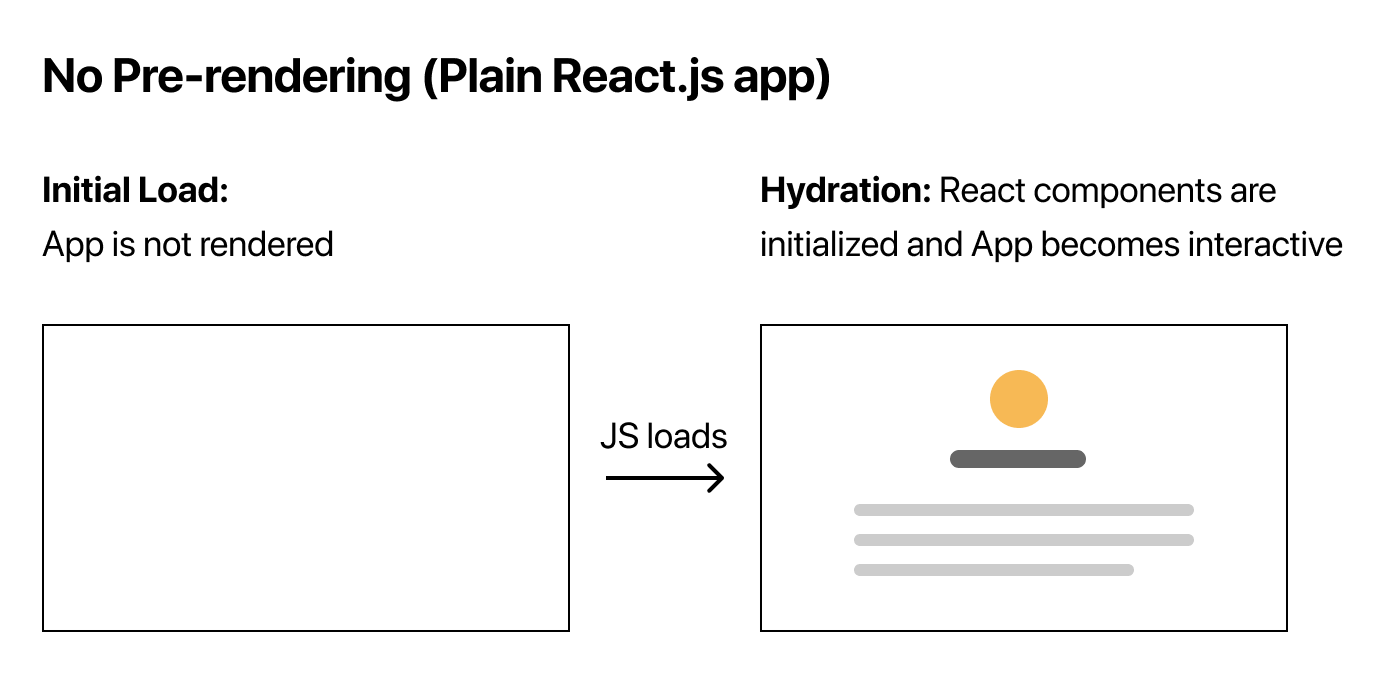
\includegraphics[width=0.45\textwidth]{Nextjs/NoPrerender}}
         \subfloat[Con Pre-rendering]{
          \label{f:nextjs_prerendering}
           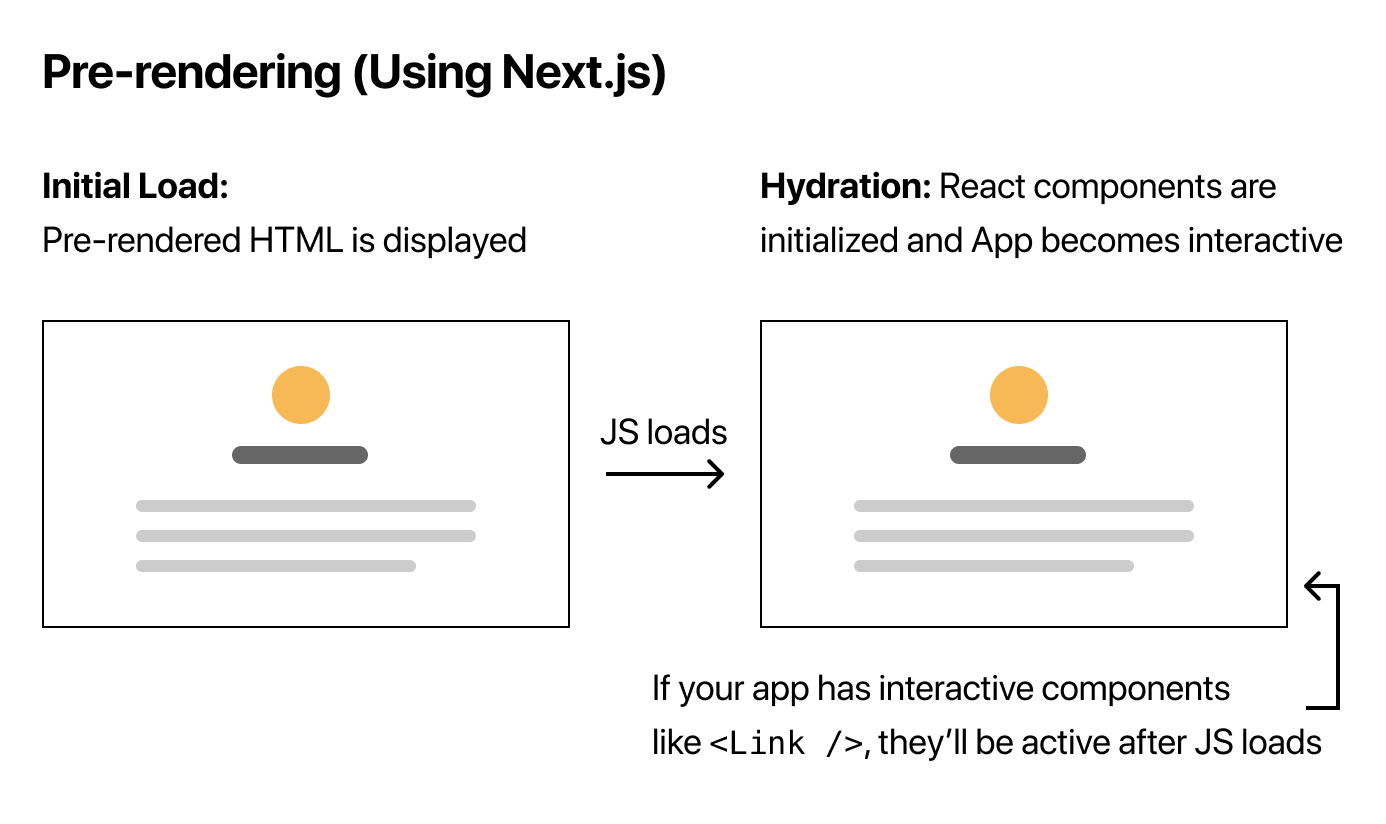
\includegraphics[width=0.45\textwidth]{Nextjs/Prerender}}
        \caption{Prerendering}
        \label{f:Prerendering}
       \end{figure}

       La renderización previa puede resultar en un mejor rendimiento y SEO. Cuando llegue el robot de Google podremos entregarle el contenido ya renderizado y esto nos permitirá posicionar igual de bien que una web estática.

    \begin{figure}[H]
        \centering
        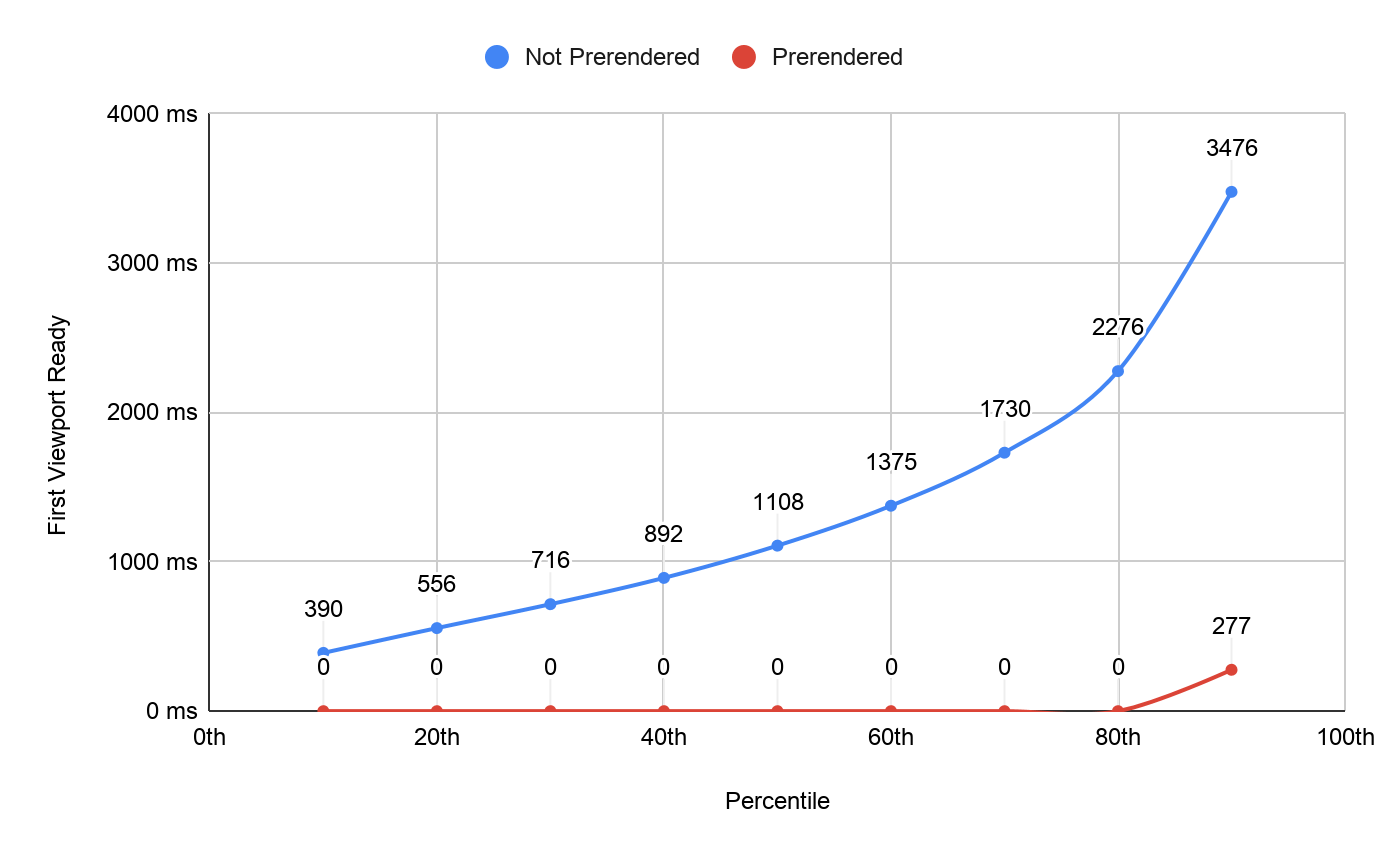
\includegraphics[scale=0.16]{Nextjs/PrerenderComparation}
        \label{fig:nextjs_prerenderinggraph}
        \caption{Time to Interactive}
    \end{figure}
    

    Next.js tiene dos formas de pre-rendering:
    \begin{itemize}
        \item **Server-side Rendering:** El HTML se genera en cada solicitud.
        \item **Generación Estática:** El HTML se genera en el momento de la compilación y se reutilizará en cada solicitud. Esta forma fue la utilizada por razones de rendimiento.
    \end{itemize}
    \begin{figure}[H]
        \centering
         \subfloat[Server-side Rendering]{
          \label{f:nextjs_ssr}
           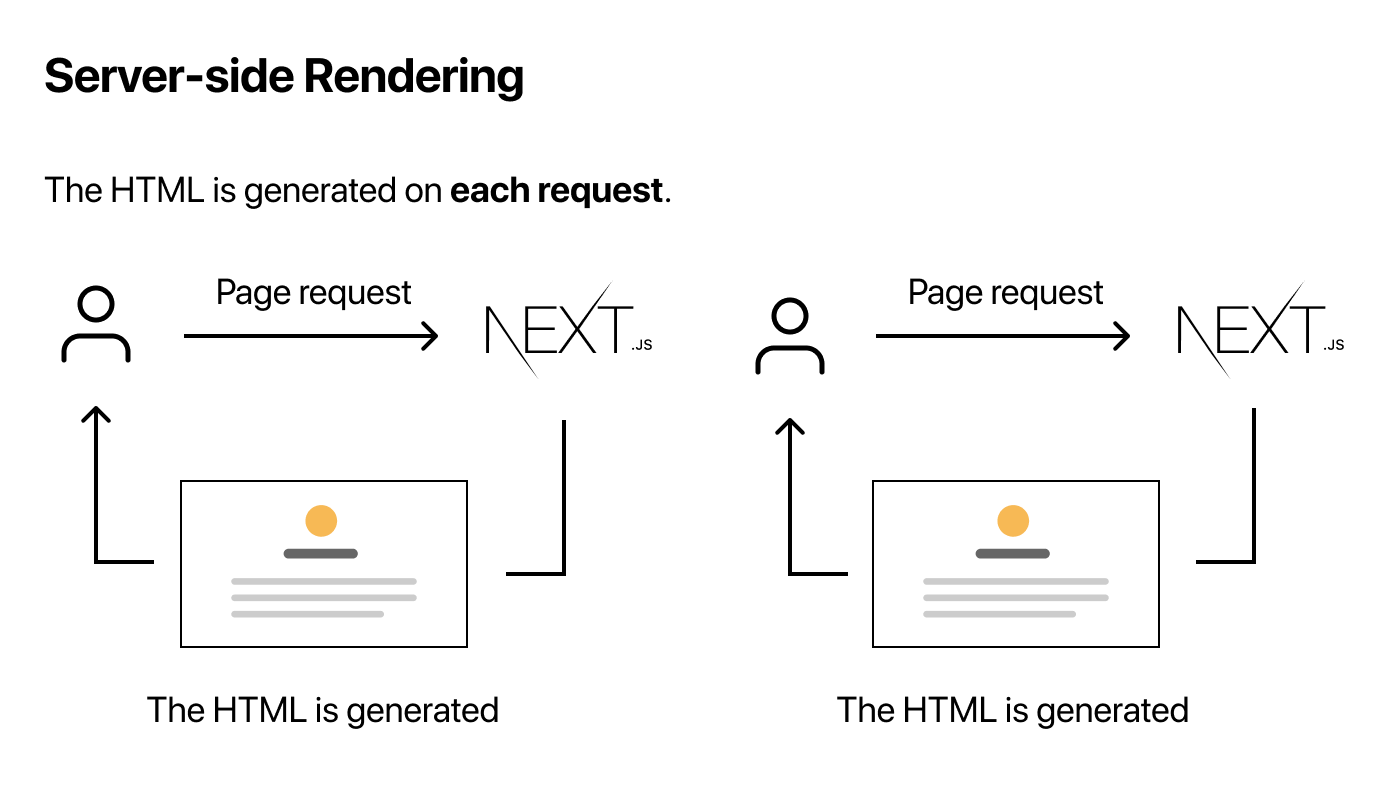
\includegraphics[width=0.45\textwidth]{Nextjs/SSR}}
         \subfloat[Generación Estática]{
          \label{f:nextjs_ssg}
           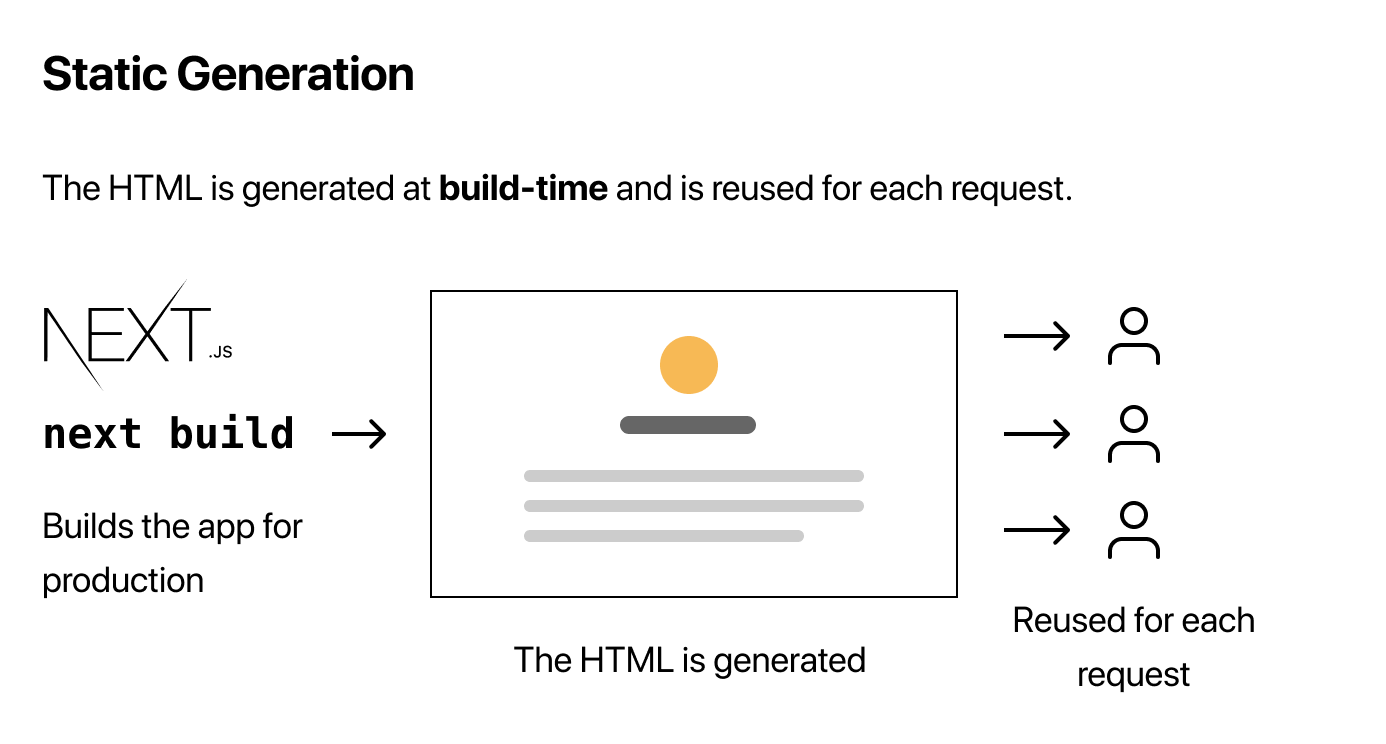
\includegraphics[width=0.45\textwidth]{Nextjs/SSG}}
        \caption{Tipos de Pre-rendering}
        \label{f:TiposPrerendering}
       \end{figure}

    \item Separación automática de código (**Code Splitting**) para cargas de página más rápidas.
        \begin{figure}[H]
            \centering
            \subfloat[Sin Code Splitting]{
            \label{f:nextjs_nocodesplit}
            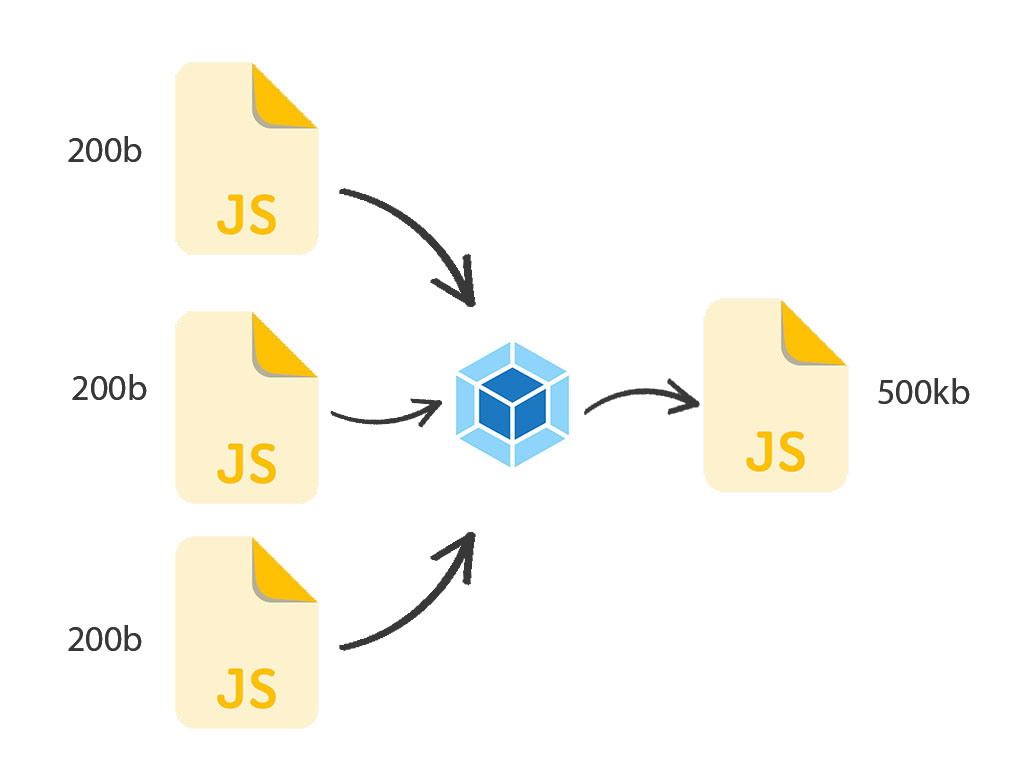
\includegraphics[width=0.4\textwidth]{Nextjs/NoCodeSplit}}
            \subfloat[Con Code Splitting]{
            \label{f:nextjs_codesplit}
            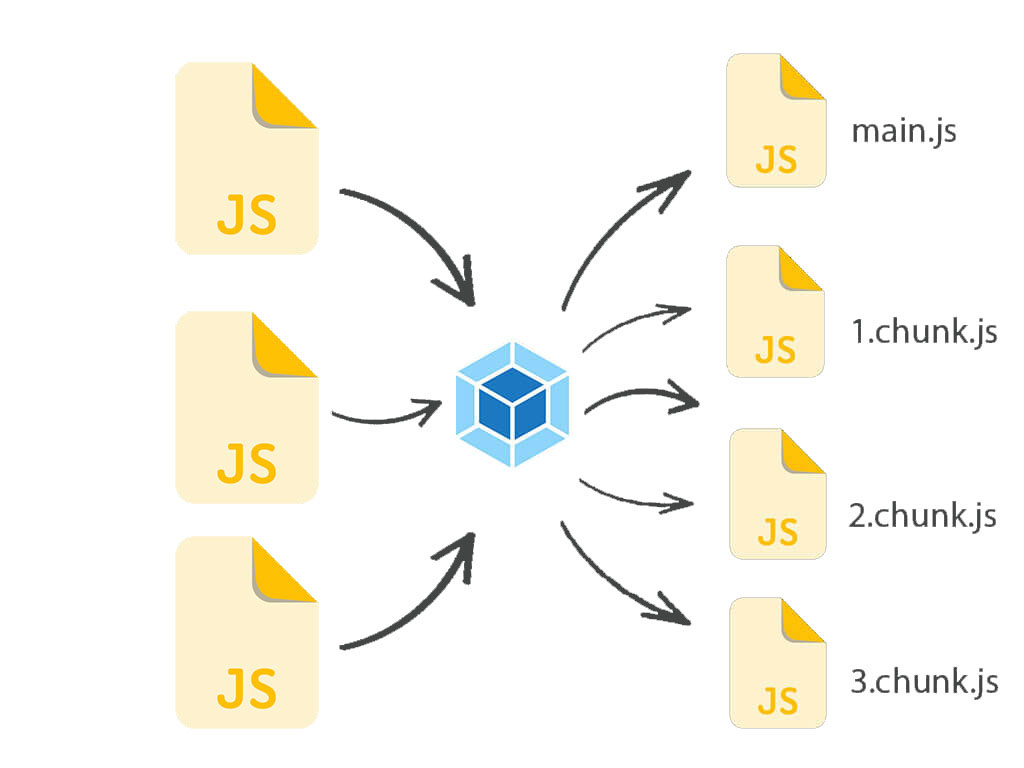
\includegraphics[width=0.4\textwidth]{Nextjs/CodeSplit}}
            \caption{Code Splitting}
            \label{f:codesplit}
        \end{figure}
    \item Enrutamiento optimizado con prefetching para Single-page Application: se precargan los elementos mostrados en la página actual.
        \begin{figure}[H]
            \centering
            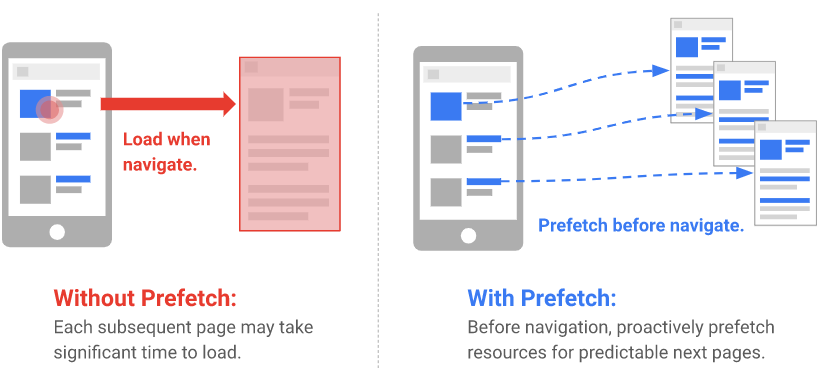
\includegraphics[scale=0.45]{Nextjs/Prefetch}
            \label{fig:nextjs_prefetch}
            \caption{Pre-fetching}
        \end{figure}
    \item Entorno de desarrollo con soporte **Fast Refresh** y **HMR** (Hot Module Replacement): Permite actualizar todo tipo de módulos y componentes de React en tiempo de ejecución sin necesidad de un refresco completo.
        \begin{figure}[H]
            \centering
            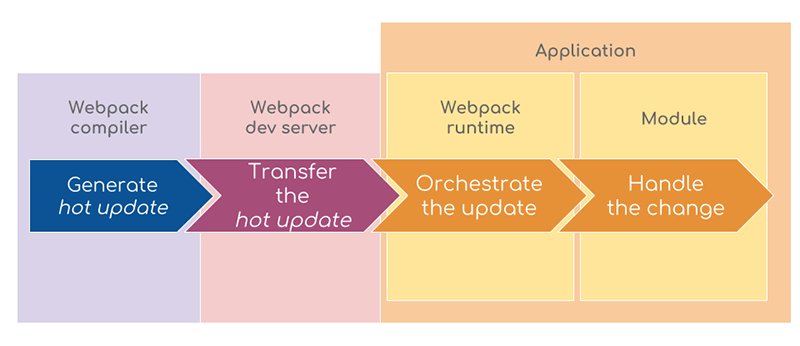
\includegraphics[scale=0.45]{Nextjs/FastRefresh}
            \label{fig:nextjs_hmr}
            \caption{Fast Refresh}
        \end{figure}    
    \item Soporte integrado de **CSS y Sass**, y soporte para cualquier biblioteca **CSS-in-JS**. (completar)
    \item **Rutas API** para crear endpoints con Serverless Functions: Cualquier archivo dentro de la carpeta pages/api se asigna a /api/* y se tratará como un endpoint en lugar de una página.
    \item Soporte para **TypeScript** completamente integrado. 
\end{itemize}

Simplemente instalamos Next, así como React y React-dom como dependencias. Estas dos últimas son necesarias para que Next pueda trabajar sin ningún tipo de problemas.

\subsubsection{React.js}

Es una biblioteca de código abierto para proyectos de JavaScript mantenida por Facebook, que permite a los desarrolladores crear aplicaciones web e interfaces de usuario de manera rápida y sencilla. Esto es posible mediante componentes interactivos y reutilizables.

React está basado en un paradigma llamado programación orientada a componentes en el que cada componente es una pieza con la que el usuario puede interactuar. Estas piezas se crean usando una sintaxis llamada JSX permitiendo escribir HTML (y opcionalmente CSS) dentro de objetos JavaScript. Estos componentes son reutilizables y se combinan para crear componentes mayores hasta configurar una web completa.

\begin{figure}[H]
    \centering
     \subfloat[Diagrama de una página]{
      \label{f:React-components_w}
       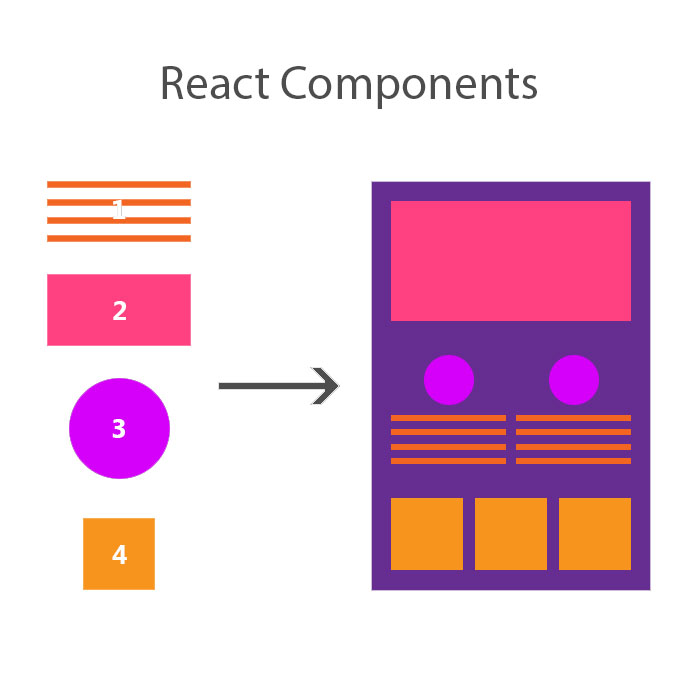
\includegraphics[width=0.4\textwidth]{Reactjs/ReactComponents}}
     \subfloat[Diagrama de un React Component]{
      \label{f:ReactComponent}
       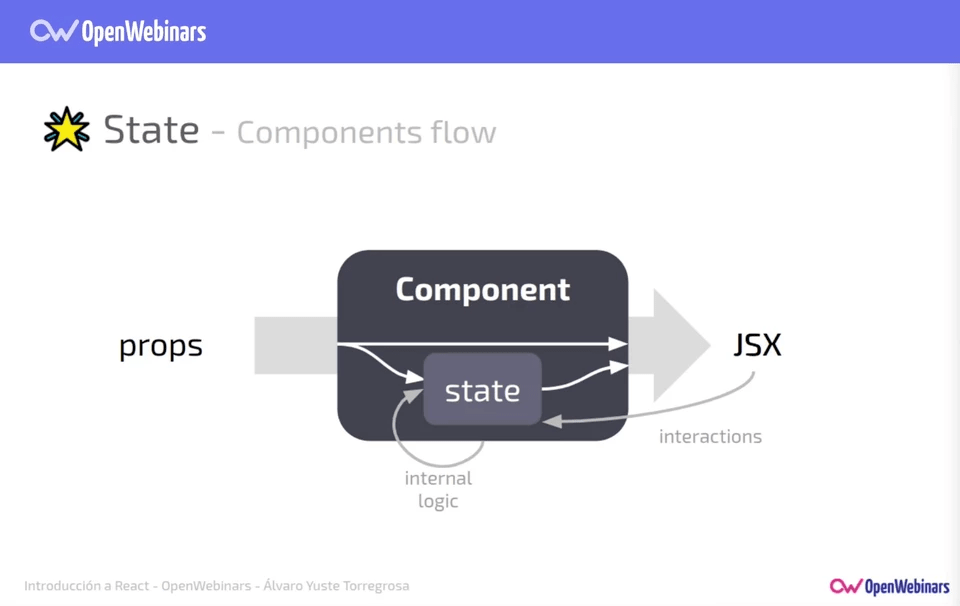
\includegraphics[width=0.45\textwidth]{Reactjs/ReactComponent}}
    \caption{React Components}
    \label{f:ReactComponents}
   \end{figure}

Además, React genera el DOM de forma dinámica, hace los cambios en una copia en memoria (DOM virtual) y después la compara con la versión actual del DOM, de esta forma evita renderizar toda la página cada vez que haya cambios, simplemente se aplica dicho cambio al componente que haya sido actualizado. Esto propicia una mejor experiencia de usuario, además de un gran rendimiento y fluidez.

\begin{figure}[H]
    \centering
    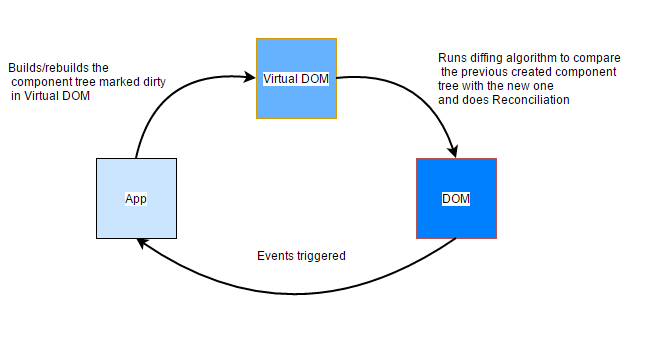
\includegraphics[scale=0.5]{Reactjs/VirtualDOM1}
    \label{fig:React_VirtualDom}
    \caption{Reconciliación Virtual DOM}
\end{figure}

Esta es la forma de tener HTML con toda la funcionalidad de JavaScript y CSS centralizado y listo para ser abstraído y usado en cualquier otro proyecto.

\subsubsection{Vercel}

Es una plataforma en la nube que permite a los desarrolladores alojar sitios web y servicios web que escalan automáticamente y no requieren supervisión. Fue creada por los desarrolladores de Next.js por lo que desplegar una aplicación con este framework tiene las siguientes ventajas:

\begin{compactitem}
    \item Las páginas que usan generación estática y assets (JS, CSS, imágenes, fuentes, etc.) se publican automáticamente desde el Vercel Edge Network, que es increíblemente rápido.
    \item Las páginas que usan pre-rendering y rutas API se convierten automáticamente en Serverless Functions. Esto permite que el renderizado de páginas y las solicitudes API puedan escalar infinitamente.
\end{compactitem}

Aparte ofrece muchas más funciones, como: dominios personalizados, variables de entorno, HTTPS automático y una vista previa de cada rama de Github por cada subida de código.

\begin{figure}[H]
    \centering
    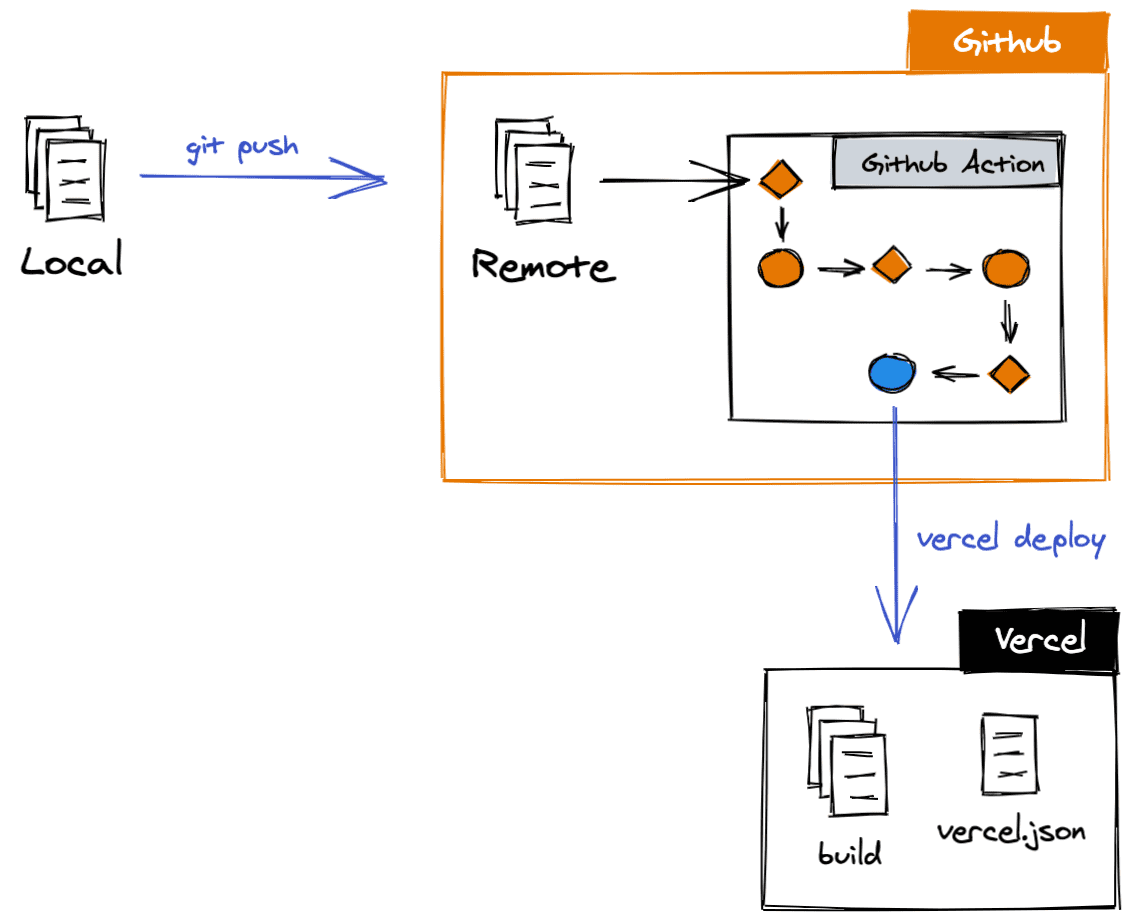
\includegraphics[scale=0.2]{Vercel/DPS}
    \label{fig:vercel_workflow}
    \caption{Flujo de trabajo DPS}
\end{figure}

Usar Nextjs junto con Vercel nos permite seguir el flujo de trabajo DPS: Develop, Preview and Ship (Desarrollo, Vista previa y Enviar a producción).

\begin{compactitem}
    \item Desarrollo: escribimos código en Next.js y usamos su servidor de desarrollo para aprovechar su función de fast refresh.
    \item Vista previa: subimos los cambios a una rama en GitHub y Vercel crea un despliegue que estará disponible a través de una URL. Podemos compartir esta URL con otros para recibir feedback.
    \item Enviar a Producción: fusionamos la rama creada con la rama main para enviar a producción.
\end{compactitem}

\subsection{TypeScript}

TypeScript es un lenguaje de programación libre y de código abierto desarrollado y mantenido por Microsoft. Es un superconjunto de JavaScript, que esencialmente añade tipos estáticos y objetos basados en clases.

Como TypeScript es un superconjunto de JavaScript, todo el código escrito en JavaScript es válido para TypeScript. Pero lo contrario no es cierto. Es decir, como los navegadores no entienden TypeScript, es necesario transpilarlo a JavaScript antes de usarlo en un navegador. Al crear nuestra aplicación con Nextjs ya obtenemos compilación y empaquetado automáticos (con webpack y babel).

\begin{figure}[H]
    \centering
    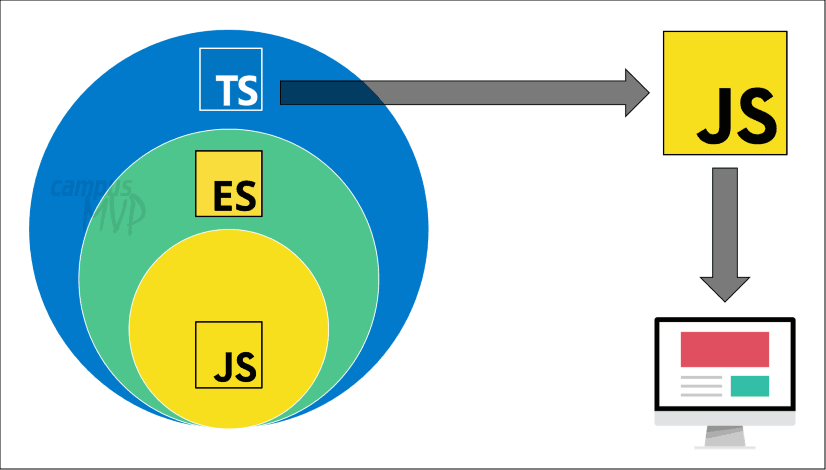
\includegraphics[scale=0.4]{TypeScript/TypeScript}
    \label{fig:TypeScript}
    \caption{TypeScript}
\end{figure}

Promueve que se escriba un lenguaje más robusto y fácil de mantener. Por lo que es un lenguaje más limpio. Permite escribir código con menos errores, más sencillo, coherente y fácil de probar. Además, ayuda a implementar patrones de diseño SOLID e incrementa la agilidad en el refactoring del código.

\subsection{Node.js}

Node.js es un entorno de tiempo de ejecución de JavaScript (de ahí su terminación en .js haciendo alusión al lenguaje JavaScript). Este entorno incluye todo lo que se necesita para ejecutar un programa escrito en JavaScript. Orientado a eventos asíncronos, Node.js está diseñado para crear aplicaciones escalables.

Permite utilizar un único lenguaje de programación para el Backend y el FrontEnd. Además cuenta con un repositorio de código abierto lleno de librerías útiles lo que ayuda en el desarrollo a una generación rápida de un producto mínimo viable.

Debemos tenerlo instalado con NPM o Yarn los cuales son unos gestores de paquetes para trabajar con proyecto de Node.js. Es necesario instalar una extensión para VScode y comenzar un proyecto nuevo con NPM o Yarn e instalar algunas dependencias necesarias como las de Typescript.

\begin{figure}[H]
    \centering
    
\includegraphics[scale=0.1]{Nodejs/NodeNPMYarn}
    \label{fig:NodeNPMYarn}
    \caption{Nodejs, NPM y Yarn}
\end{figure}

\subsubsection{NPM o Yarn}

A veces, la instalación de paquetes con NPM no es lo suficiente consistente o rápida, dando incluso a errores. Es por ese el motivo que en este proyecto se tuvo que cambiar a Yarn, que es una alternativa construida por Facebook, Google, Exponent y Tilde.

En package.json, el archivo donde tanto NPM como Yarn hacen un seguimiento de las dependencias del proyecto, los números de versión no siempre son exactos. En su lugar, se puede definir una gama de versiones.

Cada vez que se añade un módulo, Yarn crea o actualiza un archivo yarn.lock.
De esta manera se puede garantizar que en otra máquina se pueda instalar exactamente el mismo paquete, sin dejar de tener una gama de versiones permitidas definidas en package.json. 
Lo cual nos permitió resolver algunos errores en la instalación de librerias.

\subsection{VSCode}

Visual Studio Code es un editor de código redefinido y optimizado para crear y depurar aplicaciones web y en la nube modernas. Incluye soporte para la depuración, control integrado de Git, resaltado de sintaxis, finalización inteligente de código, fragmentos y refactorización de código.

Gracias a su integración de Git es sencillo revisar las diferencias, preparar los archivos y realizar confirmaciones directamente desde el editor antes de subirlo al repositorio en la nube.

Además cuenta con una biblioteca de extensiones, las cuales nos da un sin número de opciones para ser más eficiente a la hora de estar programando. Desde extensiones de otros lenguajes de programación como diferentes herramientas para visualizar o estructurar el código de manera más eficiente.

Las extensiones más importantes para mejorar la experiencia de desarrollo y buenas prácticas de este proyecto fueron ESLint y Prettier. Configurar estas herramientas será una inversión que haremos una vez y sus beneficios los notaremos durante todo el proyecto

\begin{figure}[H]
    \centering
    
\includegraphics[scale=0.8]{VSCode/VScodeExtensions}
    \label{fig:VScode_extensions}
    \caption{ESLint, Prettier y VSCode}
\end{figure}

\subsubsection{ESLint}

ESLint es una herramienta de análisis de código para identificar patrones problemáticos que se puede instalar como extensión en VSCode.

Su función es analizar el código de nuestra aplicación, detectar problemas por medio de patrones y si está a su alcance resolverlos. Se pueden usar guías de estilo cómo Airbnb, Standard o Google, pero en este caso lo vamos a configurar con la guía de estilo recomendada de ESLint y añadiremos reglas para TypeScript y React. Lo que nos permitirá:

\begin{compactitem}
 \item Corregir errores de sintaxis
 \item Corregir código poco intuitivo o difícil de mantener
 \item Evitar el uso de "malas practicas"
 \item Hacer uso de un estilo de código consistente.
\end{compactitem}

ESLint está diseñado para ser flexible y configurable por lo que añadimos ejecutar ESLint como parte del proceso de integración continua.

\subsubsection{Prettier}

Prettier es un formateador de código que puede instalarse como extensión en VSCode. Aplica un estilo consistente analizando el código y formateándolo con sus propias reglas que toman en cuenta la longitud máxima de línea, ajustando el código cuando es necesario.

Para ello, analiza el código y lo da formato cada vez que se guarda el archivo. Su objetivo es acabar con los debates sobre el estilo del código. Para usarlo junto con ESLint hay que configurar este último para que use Prettier.

En definitiva, Prettier se usa para problemas de formato de código y ESLint para problemas de calidad de código.

\section{Detalles de Implementación}
\subsection{Arquitectura}
\begin{figure}[H]
    \centering
    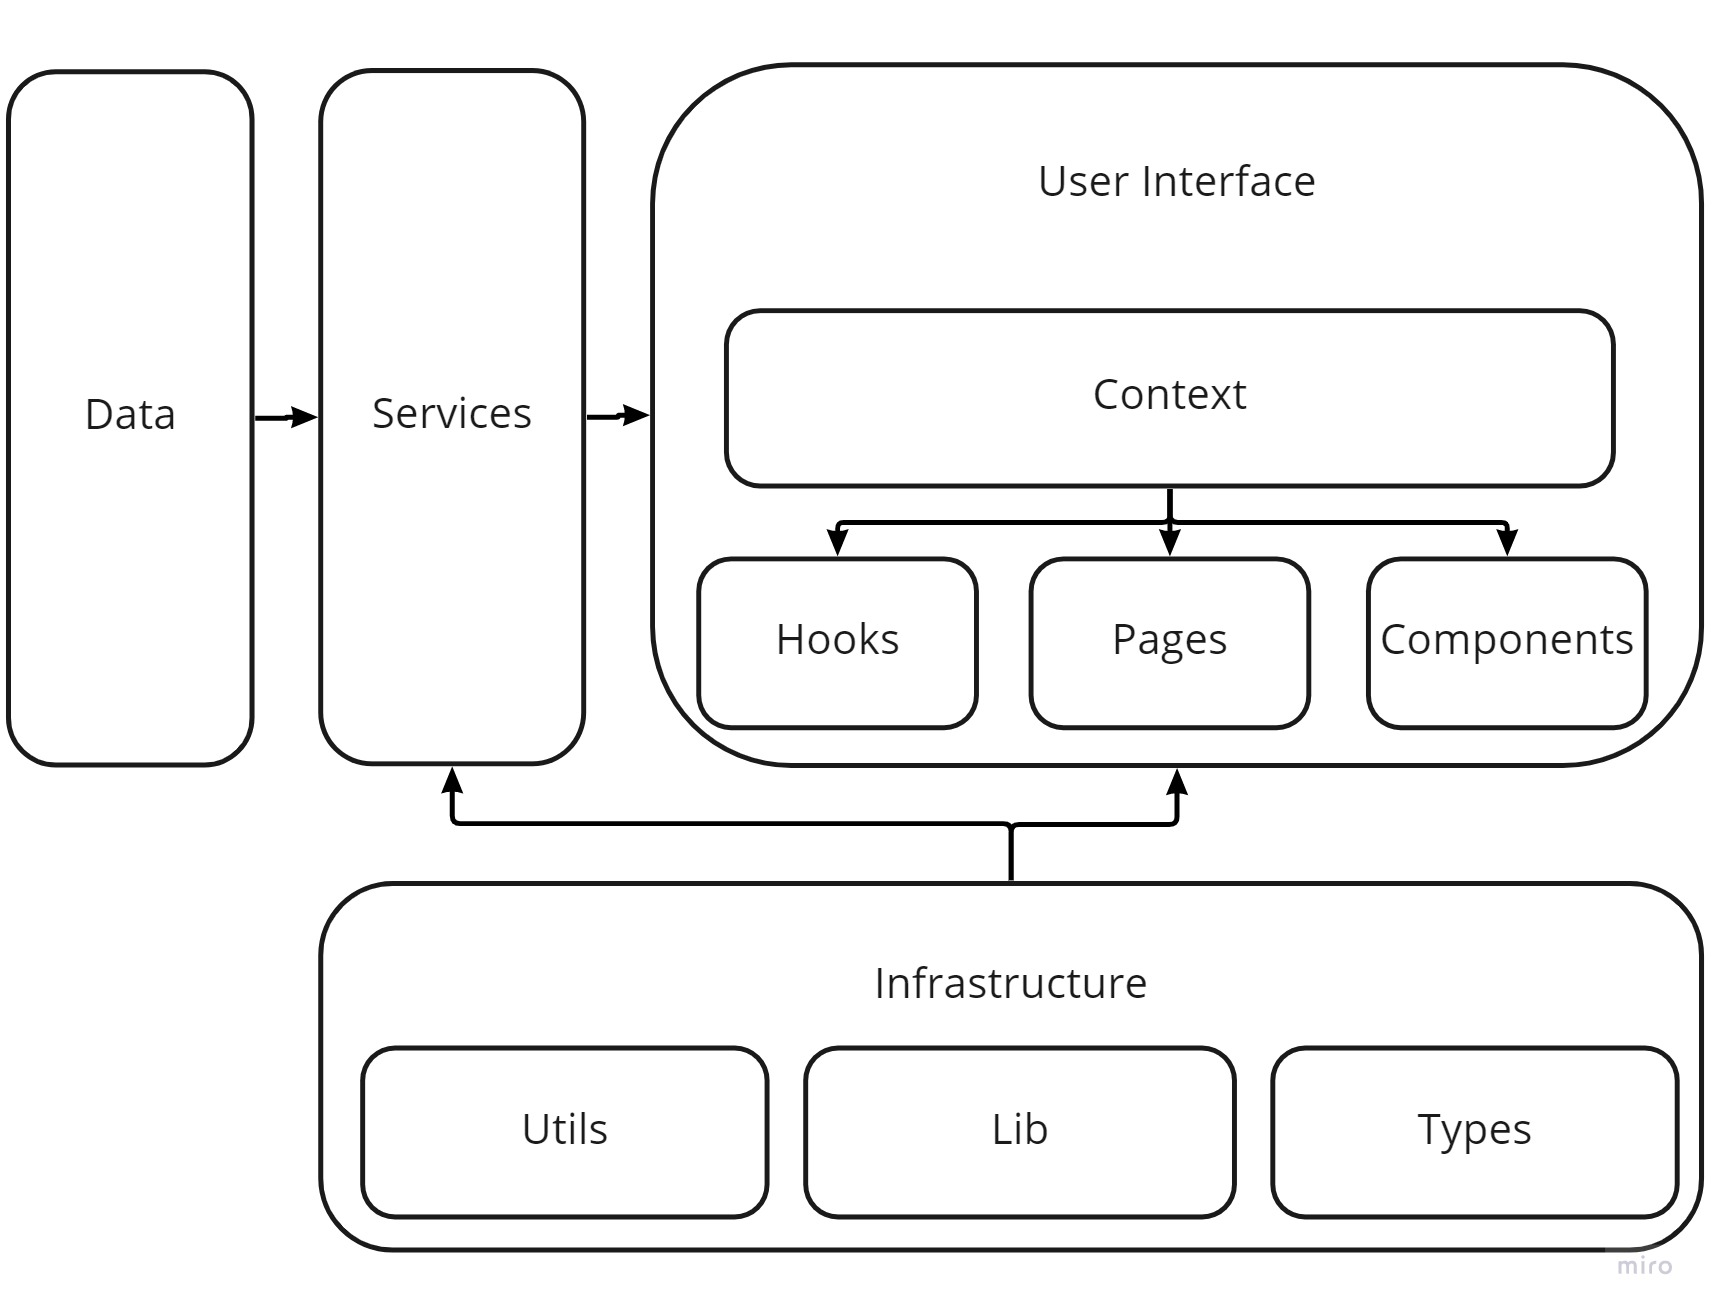
\includegraphics[scale=0.25]{Detalles de Implementación/Arquitectura}
    \label{fig:Arquitectura}
    \caption{Arquitectura}
\end{figure}

\subsection{Estructura de Archivos}

React no tiene opiniones sobre cómo poner los archivos en carpetas. Una forma popular de estructurar proyectos es agrupar archivos similares.

Nextjs en cambio tiene algunos archivos y directorios especiales. Como mínimo, se necesita una carpeta 'pages' y un archivo 'index.js' dentro de él. Además, la carpeta 'public' tiene una función específica en Nextjs. Aparte de estos archivos y directorios, todo vale.

En este caso se han separado los archivos por conceptos o intereses, donde cada carpeta se enfoca en un concepto concreto:

\begin{figure}[H]
    \centering
    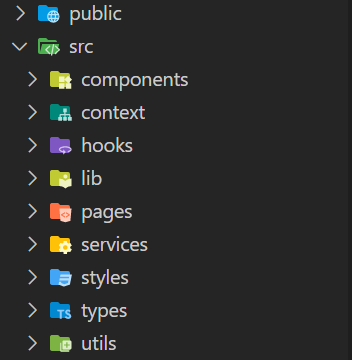
\includegraphics[scale=0.6]{Detalles de Implementación/Archivos}
    \label{fig:Archivos}
    \caption{Estructura de Archivos}
\end{figure}

\begin{itemize}
    \item \textbf{Pages}: En Next.js, una página es un componente de React exportado desde un archivo .js, .jsx, .ts o .tsx en el directorio 'pages'. Cada página está asociada con una ruta basada en su nombre de archivo. Ejemplo: En 'pages/notes' se exporta un componente de React que será accesible en '/notes'.

    Aquí se encuentran todas las páginas de la aplicación y además se encuentran los archivos '\_app.tsx' y '\_document.tsx' personalizados. 
    
    Para tener un Layout persistente para toda la aplicación, se puede crear un archivo '\_app.tsx' personalizado y envolver la aplicación con el componente. También se encuentran aquí los metadatos de la aplicación. Por otro lado, en el archivo '\_document.tsx' se pueden actualizar las etiquetas '<html>' y '<body>', por ejemplo añadiendo 'lang='en'' a la etiqueta '<html>'. 
    \item \textbf{Public}: Next.js puede servir archivos estáticos, como imágenes, en una carpeta llamada 'public' en el directorio raíz. El código puede hacer referencia a los archivos dentro de 'public' a partir de la URL base (/). Aquí se pueden encontrar los iconos, imágenes y archivos de fuente de sonido (soundfonts en formato MIDI.js) de la aplicación.
    \item \textbf{Components}: El modelo React nos permite deconstruir una página en una serie de componentes. Muchos de estos componentes a menudo se reutilizan entre páginas. Aquí se pueden encontrar todos los componentes de la aplicación agrupados por carpetas.
    \item \textbf{Types}: Para usar Typescript todos los archivos '.js' se convierten en '.ts' y '.jsx' en '.tsx'. Aquí se encuentran en un archivo todos los tipos personalizados usados en los demás archivos de la aplicación.
    \item \textbf{Lib}:  Aquí se puede encontrar 'soundfont-wrapper', una librería personalizada para la aplicación. Para hacer uso de la librería 'soundfont-player', que se encarga de cargar los archivos de fuente de sonido (soundfonts) y reproducir sonidos MIDI utilizando la WebAudio API.  Se decidió crear esta librería envoltorio (Wrapper library) para refinar la complejidad de su interfaz y simplificar su uso.
    \item \textbf{Utils}: Aquí se pueden encontrar archivos con métodos genéricos para ser usados en cualquier parte de la aplicación. Por ejemplo: en 'arrayUtils.ts' está el método 'getRandomItem' que devuelve un elemento al azar de un array.
    \item \textbf{Styles}: Aquí se pueden encontrar algunos estilos css globales para la aplicación. Aunque en general se hace uso de 'react-bootstrap' junto con 'bootswatch' para los estilos de la aplicación.
    \item \textbf{Services}: Los servicios proporcionan los datos y un conjunto de métodos responsables de alguna lógica específica siendo independientes de la capa IU. Aquí puedes encontrar los servicios que son consumidos desde los Hooks.
    \item \textbf{Context}: El Context está diseñado para compartir datos que pueden considerarse “globales” para un árbol de componentes en React. Como es un componente algo especial, como las pages, tiene su propio directorio.
    \item \textbf{Hooks}: Los Hooks son una nueva característica en React 16.8. Estos permiten usar el estado y otras características de React sin escribir una clase. Aquí puedes encontrar todos los Custom Hooks creados, para extraer la lógica de los componentes en funciones reutilizables.
\end{itemize}

\subsection{Infraestructura}
\subsection{Datos y Servicios}
\subsection{Componentes y Pages}
\begin{figure}[H]
    \centering
    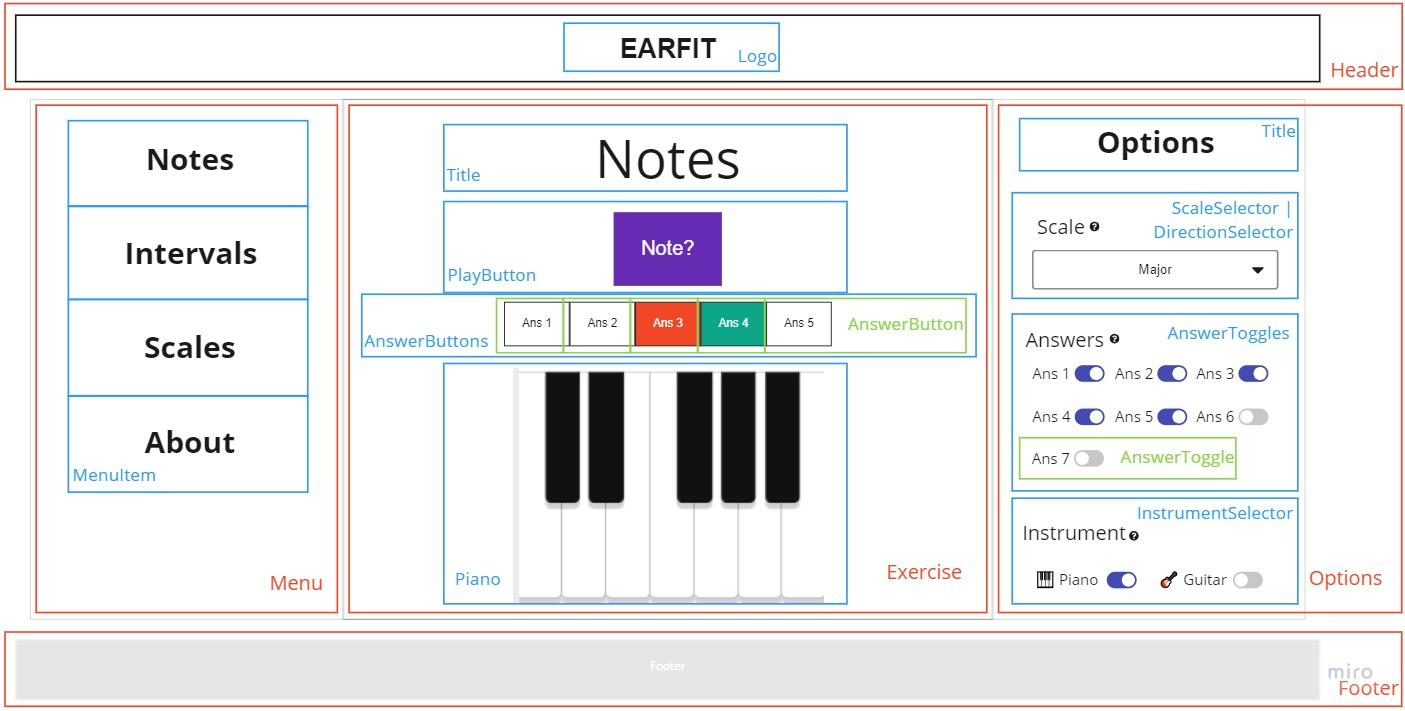
\includegraphics[scale=0.28]{Detalles de Implementación/JerarquíaComponentes}
    \label{fig:JerarquíaComponentes}
    \caption{Jerarquía de Componentes}
\end{figure}
\subsection{Hooks y Context}

\subsection{Progressive Web App}
Para conseguir que una aplicación web sea confiable, instalable y se comporte como una app nativa en ordenador, móvil y tablet se puede convertir en Progressive Web App. Con la Progressive Web App, el usuario puede instalar la app en su dispositivo y seguir consultándola, aunque haya perdido la conexión.

Para poder llamar PWA a una aplicación web, debe tener las siguientes características:

\begin{compactitem}

    \item \textbf{Una conexión segura:} La aplicación web se debe servir a través de una red segura HTTPS.
    \item \textbf{Cargue sin conexión:} Esto significa que las aplicaciones web progresivas requieren de un \textbf{service worker}.
    \item \textbf{Información sobre la aplicación:} como nombre, autor, icono y descripción en un documento JSON llamado \textbf{manifest}.
    \item \textbf{Un icono} de al menos 144x144 de tamaño grande en formato PNG.
\end{compactitem}

Siendo una PWA, al visitarla cualquier navegador ya nos da la opción de instalarla en nuestro dispositivo. En iOS, la opción se llama 'añadir a pantalla de inicio' desde el menú 'compartir' de Safari y en Chrome por ejemplo es de la siguiente manera:

\begin{figure}[H]
    \centering
    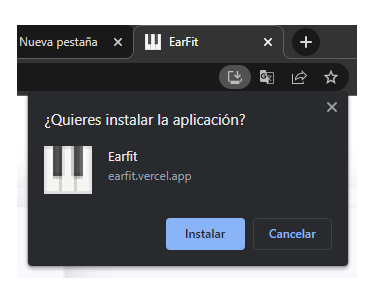
\includegraphics[scale=0.9]{Detalles de Implementación/InstalarPWA}
    \label{fig:InstalarPWA}
    \caption{Instalar PWA desde Chrome}
\end{figure}

Al instalarla se crea un icono en la pantalla de inicio y ya está lista para usar. Puede usarse sin conexión y en cualquier tamaño de ventana ya que al ser responsiva se adapta. Para desinstalar se puede hacer como una aplicación normal o simplemente pulsando en los tres puntos de la ventana nos da la opción.

\begin{figure}[H]
    \centering
    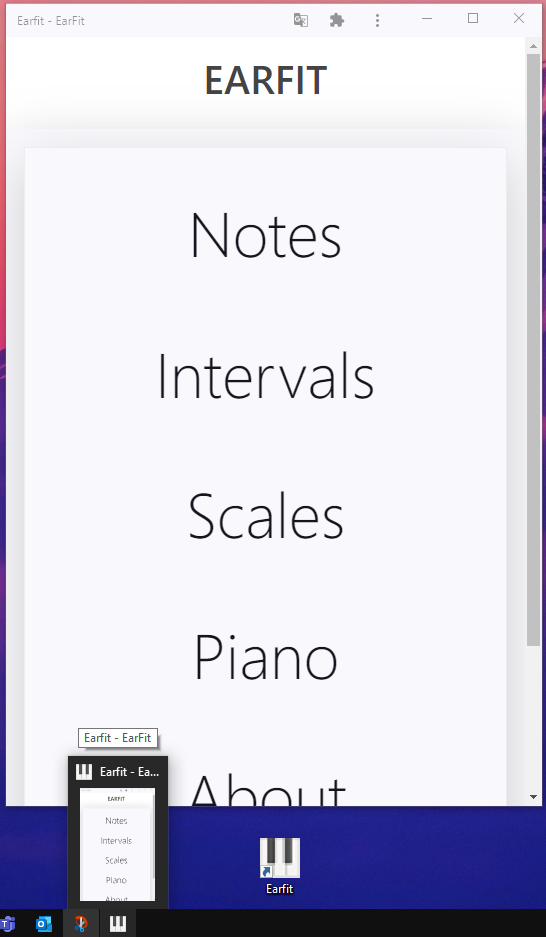
\includegraphics[scale=0.28]{Detalles de Implementación/PWA}
    \label{fig:PWA}
    \caption{Earfit como PWA en Windows}
\end{figure}

Observación: En el entorno desarrollo, se ha deshabilitado la opción de PWA en next.config.js porque genera muchos mensajes de consola.

\subsubsection{Service Worker}
Se puede encontrar en la carpeta public con el nombre de sw.js. Es un script que permite interceptar y controlar cómo un navegador web maneja las solicitudes de red y el almacenamiento en caché. Este es un archivo autogenerado mediante el plugin next-pwa, que permite registrar y generar un service worker optimizado sin apenas configuración. El archivo workbox también está relacionado con este plugin.

\subsubsection{Manifest}
Se puede encontrar en la caperta public con el nombre de manifest.json. Es un archivo que controla cómo se muestra la aplicación al usuario y garantiza que las PWA sean detectables. Describe el nombre de la aplicación, la URL de inicio, los iconos y todos los demás detalles necesarios para transformar el sitio web en un formato similar al de una aplicación. 

IOS Safari no implementa manifiestos, por lo que la mayoría de los metadatos de PWA se pueden definir a través de extensiones específicas de Apple para las metaetiquetas. Estos están definidos en el archivo personalizado '\_app.tsx'

Los iconos de la aplicación a los que se hacen referencia se pueden encontrar en la carpeta 'public/icons'.


\subsection{Buenas Prácticas}

Al hablar de buenas prácticas en programación nos referimos a un conjunto de técnicas, principios, metodologías que debemos implementar en nuestro software para que se vuelva fácil, rápido y seguro de desarrollar, mantener y desplegar.

\subsubsection{Guía de Estilo de Código}

Se han usado las reglas recomendadas de ESLint y Prettier. Las reglas se pueden encontrar en el archivo `.eslintrc.js` y `.prettierrc.js`. Además se han añadido las siguientes reglas personales:

\begin{compactitem}
    \item Tipos de TypeScript para los componentes en lugar de `props`.
    \item No es necesario importar React cuando se usa Next.js
    \item Desactivar la regla para enlaces predeterminada, no es compatible con los componentes `<Link />` de Next.js
    \item Eliminar variables sin usar
    \item Las funciones tienen que devolver siempre un tipo.
    \item Uso de comas finales
    \item Indentación a 2 espacios
    \item Uso de comillas simples para strings
    \item Longitud de línea máximo 120 caracteres
    \item No usar tabulaciones
    \item Finales de linea automaticos (`LF` to `CRLF`).
\end{compactitem}

\subsubsection{Principios Clean Code}

Los principios de Clean Code nos permiten obtener como resultado un código limpio, reutilizable, escalable y con mayor cambiabilidad. Algunos de los principales principios que se han intentado tener presentes a la hora de desarrollar el código son:

\begin{compactitem}
    \item Follow Standard Conventions: Seguir convenciones estandarizadas.
    \item DRY Principle (Don't Repeat Yourself): No repetir código
    \item The Principle of Least Surprise: Las funciones o clases deben hacer lo que se espera que hagan.
    \item The Boy Scout Rule: Dejar el código más limpio de como te lo encontraste.
    \item Keep It Simple Stupid: Reducir la complejidad tanto como sea posible.
    \item You Are Not Gonna Needed: Sólo se debe añadir el código que sea estrictamente necesario.
    \item Choose Descriptive Names: El código debe ser legible para otros desarrolladores.
    \item Be Consistent: Si haces algo de cierta manera, haz todas las cosas similares de la misma manera.
    \item Single Responsibility Principle: Las clases deben tener solo una razón para cambiar
    \item Open/Closed Principle: Las clases deben estar abiertas a extensiones pero cerrada a modificaciones
    \item Liskov Substitution Principle: Las clases derivadas deben poder sustituirse por sus clases base
    \item Interface Segregation Principle: Hacer interfaces que sean específicas para un tipo de cliente
    \item Dependency Inversion Principle: Depende de abstracciones, no de clases concretas (nuestras clases deben depender de abstracciones, nunca de detalles concretos).
\end{compactitem}

\subsubsection{Otras Buenas Prácticas}

\begin{compactitem}
    \item Visualizar el flujo de trabajo.
    \item Limitar el trabajo en proceso (Work in Progress) mediante un sistema de arrastre (pull) sobre el flujo de trabajo. Es decir no multitasking.
    \item Circuitos de retroalimentación: reuniones periódicas.
    \item Fomentar la visibilidad. No se puede mejorar algo que no se entiende. Esta es la razón por la cual el proceso debe estar bien definido, publicado y promovido.
    \item Mejorar colaborando, usando modelos y el método científico.
    \item Calidad perfecta a la primera: Búsqueda de cero defectos, detección y solución de los problemas en su origen.
\end{compactitem}

\section{Testing}

El testing de software o software QA, es un proceso para verificar y validar la funcionalidad de un programa o una aplicación de software. Su propósito principal es asegurar que la aplicación desarrollada cumpla con los estándares y se ofrezca al cliente un producto de calidad.

\subsection{Pruebas Funcionales}

El objetivo de estas pruebas es evaluar las suposiciones hechas en las especificación de requisitos y diseño para asegurar que el software se comporta según lo definido.

Estas pruebas se realizaron de forma manual interactuando con el software. Dado que es una aplicación pequeña y el desarrollo de pruebas automáticas tiene asociado un coste de implementación y mantenimiento. Por lo que hay que llegar a un compromiso de valor aportado (defectos que no llegan a producción) frente al coste de desarrollarlas. 

En cada tipo de prueba el SUT ****(Subject under Test - Sujeto bajo Prueba) se define siempre desde su perspectiva. Cada una pretende abordar un objetivo en concreto donde se han intentado probar todos los Test Cases o Casos de prueba ****posibles.

\subsubsection{Pruebas Unitarias}

Estas pruebas permiten probar que los elementos más fundamentales del software como objetos, funciones, eventos, funcionan como se espera. 

En este caso según se iba desarrollando el código se comprobaba que cada hook, función, estado, devolvía el resultado esperado y funcionaba correctamente antes de darle uso en el código. 

Realizando pequeños tests por consola y usando las herramientas para desarrolladores de Google Chrome cuando era necesario.

\subsubsection{Pruebas de Componentes}

En estas pruebas se considera el SUT como cada componente de React. Con el objetivo de probar si la funcionalidad descrita en las historias de usuario se corresponde con su comportamiento.

Permiten identificar fallos en los componentes que incluyen varias funciones o elementos internos para que se puedan corregir antes de que el software llegue a producción. 

En este tipo de pruebas se validaron los criterios de aceptación descritos en las historias de usuario. Probando cada componente según se desarrollaba. Cualquier problema detectado se reparó de forma inmediata antes de continuar con el desarrollo.

\subsubsection{Pruebas de Integración}

El objetivo es probar la interacción entre componentes al integrar uno nuevo en la aplicación. Permiten probar el comportamiento y posibles fallos en la interacción entre los componentes entre sí, y demás elementos del software.

De esta manera en cada momento tenemos una visión general del estado del proyecto alertándonos de regresiones en el código.

En este caso, al integrar un nuevo componente en la aplicación, se probó si su funcionamiento y el de los componentes con los que interactúa seguía siendo el adecuado.

\subsubsection{Pruebas End to End (E2E)}

Estas pruebas se realizaron sobre el sistema una vez desplegado desde el punto de vista de los usuarios. En estas pruebas el SUT es el sistema completo de principio a fin. Se realizan con el objetivo de verificar si el software se comporta como se espera según las historias de usuario.

Estás pruebas se han realizado con los siguientes objetivos:

\begin{compactitem}
    \item Pruebas de sanidad (sanity check): Probar las funcionalidades básicas del sistema, usadas después de un despliegue.
    \item Pruebas de instalación y desinstalación: Probar las funcionalidades básicas del sistema, después de instalarse como progressive web app.
\end{compactitem}

En este caso cada historia de usuario se probó para asegurarse de que siguen funcionando correctamente y se obtienen los resultados esperados.

\subsection{Pruebas No Funcionales}

\subsubsection{Google Lighthouse}

Google Lighthouse es una herramienta automatizada de código abierto para medir la calidad de las páginas web. Audita el rendimiento, la accesibilidad, y la optimización de páginas web.

También incluye la capacidad de probar aplicaciones web progresivas (PWA) para el cumplimiento de estándares y mejores prácticas.

Para que estas aplicaciones web progresivas (PWA) causen la sensación a los usuarios de estar manejando una aplicación nativa, deben cumplir con determinadas características y parámetros de rendimiento. El test de Lighthouse permite \textbf{medir y optimizar estos indicadores.}

Una vez hecho el análisis, Lighthouse emite \textbf{puntuaciones del 0 al 100} que pueden tomarse como guía para detectar errores potenciales u oportunidades de optimización. En nuestra aplicación las puntuaciones fueron las siguientes, sin variaciones entre unas páginas y otras:

\begin{figure}[H]
    \centering
    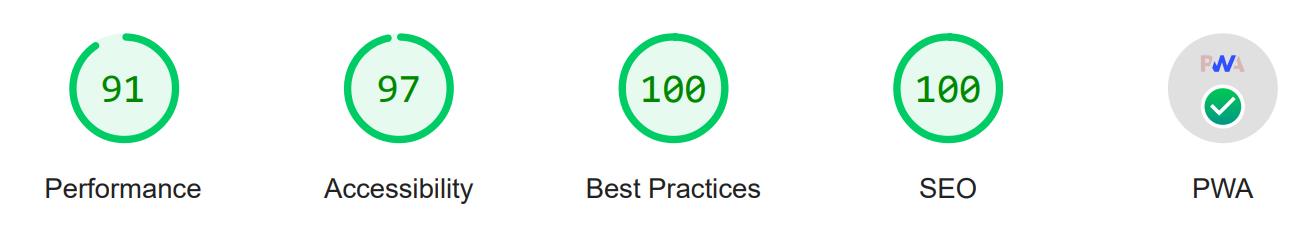
\includegraphics[scale=1.2]{Lighthouse/Resumen}
    \label{fig:Lighthouse_resumen}
    \caption{Puntuaciones de Lighthouse}
\end{figure}

\subsubsection{Performance}

En el ámbito del rendimiento, \textbf{Lighthouse analiza la velocidad} de la aplicación web y comprueba que los elementos que se han cargado se visualizan correctamente. En este apartado, Lighthouse no está optimizado y da algunos falsos positivos para aplicaciones Nextjs. Por ejemplo, con el componente Image. Sin embargo, como hemos desplegado nuestra aplicación usando Vercel, podemos hacer uso de Vercel Analytics, que además nos aporta algunas ventajas. En lugar de medir en nuestro portátil, Vercel Analytics recopila datos de los dispositivos reales que utilizan los usuarios. 

\subsubsection{Accessibility}

En el ámbito de la accesibilidad, Lighthouse comprueba si la página o la aplicación es fácil de usar para \textbf{personas con limitaciones físicas}. Se comprueba si los elementos importantes, como los botones y los enlaces, se describen de forma clara. Estos son los resultados de la aplicación final:

\begin{figure}[H]
    \centering
    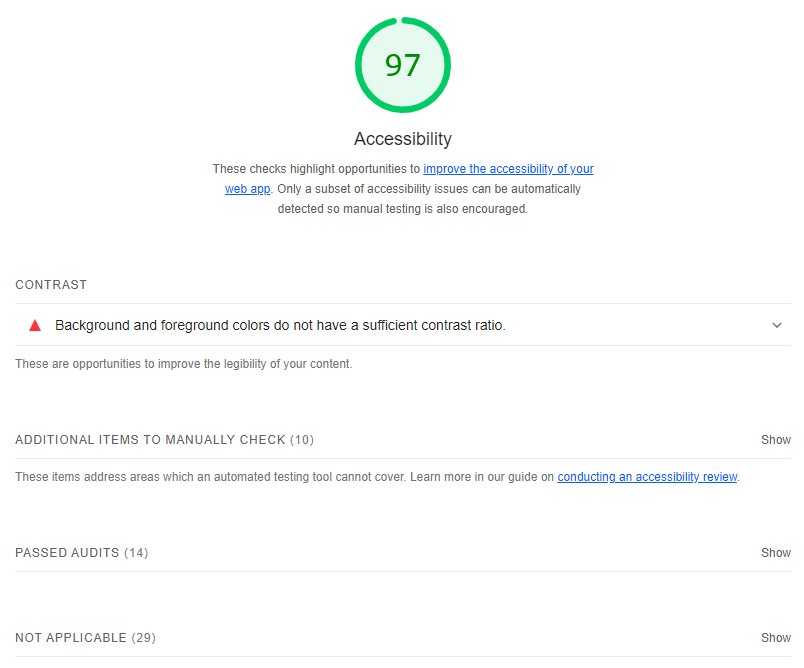
\includegraphics[scale=0.6]{Lighthouse/Accesibility}
    \label{fig:Lighthouse_accesibility}
    \caption{Accesibility}
\end{figure}

En este apartado nos resta tres puntos y nos dice que el texto del Footer tiene poco contraste. No lo tenemos en cuenta, ya que este es un mensaje secundario que no tiene que resaltar, por eso su bajo contraste.

\begin{figure}[H]
    \centering
    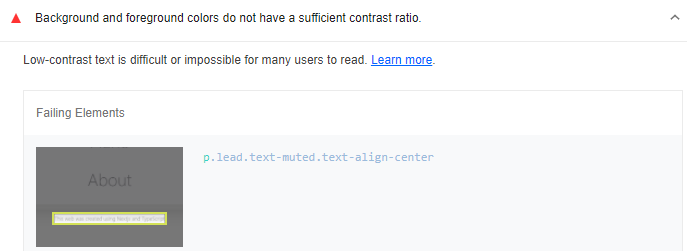
\includegraphics[scale=0.6]{Lighthouse/AccesibilityContrast}
    \label{fig:Lighthouse_contrast}
    \caption{Contrast fail}
\end{figure}

\subsubsection{Best Practices}

En el área \textbf{de mejores prácticas, Lighthouse analiza, sobre todo, los aspectos de seguridad} de la web. Aquí, la herramienta comprueba si se han usado tecnologías de codificación como TLS, si los recursos integrados de la página web provienen de fuentes seguras o si las bibliotecas JavaScript se pueden catalogar como seguras. También analiza si las bases de datos son seguras (si las hay) y destaca el uso de API anticuadas. Estos son los resultados de la aplicación final:

\begin{figure}[H]
    \centering
    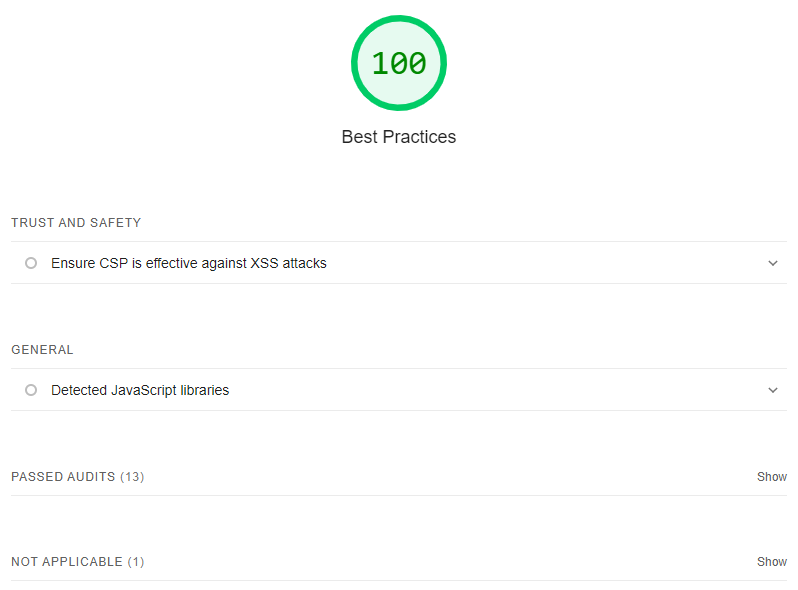
\includegraphics[scale=0.6]{Lighthouse/BestPractices}
    \label{fig:Lighthouse_bestpractices}
    \caption{Best Practices}
\end{figure}

\subsubsection{SEO}

En este ámbito Lighthouse analiza el nivel de visibilidad de la web en diferentes \textbf{buscadores}. Se comprueba especialmente la idoneidad de la web para terminales móviles, es decir, si las etiquetas y los metadatos se han optimizado. Estos son los resultados de la aplicación final:

\begin{figure}[H]
    \centering
    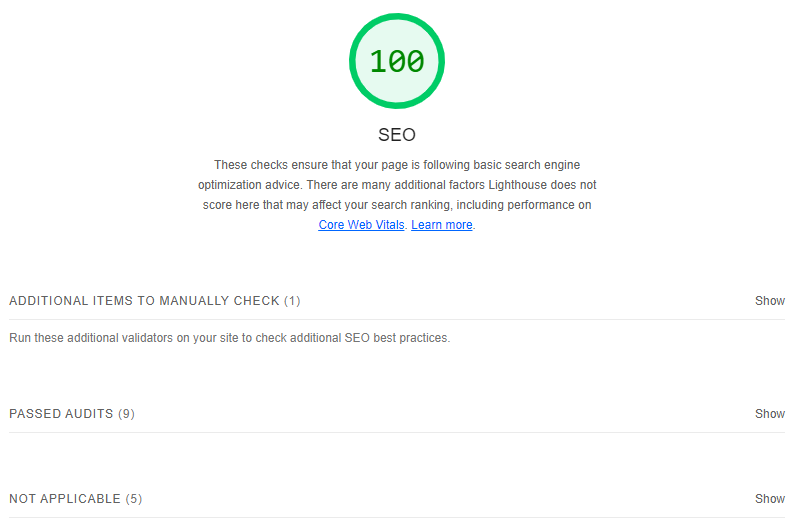
\includegraphics[scale=0.6]{Lighthouse/SEO}
    \label{fig:Lighthouse_seo}
    \caption{SEO}
\end{figure}

\subsubsection{Progressive Web Apps}

El análisis de aplicaciones web progresivas es la función principal de Google Lighthouse. El software analiza si la página web funciona según lo previsto. Comprueba \textbf{si todos los elementos y contenidos dinámicos se representan correctamente}, si la página registra un service worker y si está disponible la función offline. Un service worker es un script que se ejecuta para que determinada información de la página web también esté disponible offline. Por norma general, para este propósito suele establecerse una interfaz proxy entre la página web y el usuario. Estos son los resultados de la aplicación final:

\begin{figure}[H]
    \centering
    \includegraphics[scale=0.6]{Lighthouse/PWA}
    \label{fig:Lighthouse_PWA}
    \caption{PWA}
\end{figure}

\subsubsection{Vercel Analytics}

Mientras que otras herramientas como Lighthouse estiman la experiencia de usuario ejecutando una simulación en el ordenador del desarrollador, el Real Experience Score de Vercel se calcula utilizando datos reales recopilados de los dispositivos de los usuarios reales. Por eso, proporciona una calificación real de cómo los usuarios realmente experimentan la aplicación.

\begin{figure}[H]
    \centering
    \includegraphics[scale=0.8]{Vercel/VercelAnalyticsResume}
    \label{fig:Vercel_metrics_resume}
    \caption{Vercel Analytics}
\end{figure}

Esto permite un flujo continuo de mediciones de rendimiento, a lo largo del tiempo, integrado en el flujo de trabajo de desarrollo. Con lo que se puede correlacionar fácilmente los cambios en el rendimiento con las nuevas implementaciones.

\subsubsection{Real Experience Score}

En función de todas las métricas que se mencionan a continuación, Vercel calcula la Real Experience Score. Y nos muestra esta vista de análisis, que nos aporta información útil que permitirá mejorar la experiencia de usuario.

\begin{figure}[H]
    \centering
    \includegraphics[scale=0.5]{Vercel/RealExperienceScore}
    \label{fig:Vercel_metrics}
    \caption{Web Vitals}
\end{figure}

\subsubsection{Web Vitals}

Son una colección de métrica establecidas por Google \cite{webdev} junto con el \textbf{Web Performance Working Group} \cite{w3} que rastrean la velocidad de carga , capacidad de respuesta y estabilidad visual de una aplicación web. El análisis consta de las siguientes cuatro categorías:

\begin{itemize}
    \item\textbf{First Contentful Paint (FCP):} Mide la velocidad de carga, o cuando se muestra el primer contenido de la página.
    \item\textbf{Largest Contentful Paint (LCP):} Mide la velocidad de carga percibida, o cuando se puede visualizar todo el contenido de la página.
    \item\textbf{Cumulative Layout Shift (CLS):} Mide la estabilidad visual, o cuánto se mueven los elementos después de mostrarse al usuario. Por ejemplo, cuando un botón se mueve porque una imagen se cargó tarde, eso es CLS.
    \item\textbf{First Input Delay (FID):} Mide la capacidad de respuesta de la página, o cuánto tiempo esperan los usuarios para ver la reacción de su primera interacción con la página. Por ejemplo, la cantidad de tiempo entre el momento en que hago clic en "Agregar al carrito" y el incremento del número de artículos en el carrito es FID.
\end{itemize}

\newpage

%%%%%%%%%%%%%%%%%%%%%%%%%%%%%% 4 Conclusiones %%%%%%%%%%%%%%%%%%%%%%%%%%%%%%%%%%%%%
\chapter{Conclusiones}

En este capítulo se detallan las conclusiones derivadas del TFG y la propuesta de posibles trabajos futuros.

Qué he aprendidos
Qué debo mejorar

\blankpage



%%%%%%%%%%%%%%%%%%%%%%%%%%%%%%% Bibliografía %%%%%%%%%%%%%%%%%%%%%%%%%%%%%%%%%%%%%

\phantomsection
\addcontentsline{toc}{chapter}{Bibliografía}
\footnotesize{
%\bibliographystyle{hispa}
\bibliographystyle{IEEEtran}
\bibliography{bibliografia}
}
% No expandir elementos para llenar toda la página
\raggedbottom
\afterpage{\blankpage}
\newpage


%%%%%%%%%%%%%%%%%%%%%%%%%%%%%%% Apéndices %%%%%%%%%%%%%%%%%%%%%%%%%%%%%%%%%%%%%%%%

\appendix
\phantomsection
\addcontentsline{toc}{chapter}{Apéndices}
\mbox{}
\vfill
\begin{center}
\begin{Huge}
\textbf{Apéndices}
\end{Huge}
\end{center}
\vfill
\mbox{}
\thispagestyle{empty}
\newpage
\mbox{}
\thispagestyle{empty}
\newpage

%%%%%%%%%%%%%%%%%%%%%%%%%%%%%%% Apendices %%%%%%%%%%%%%%%%%%%%%%%%%%%%%
\chapter{Ideación y Diseño (Ampliación)}

\section{Lean Startup (Ampliación)}
\label{sec:apendice}

Para entender mejor el por qué de usar este método, explicaremos las 3 partes de las que se compone y que hemos seguido, añadiendo prácticas de Design Thinking para la construcción de nuestra solución. Lo cual ayudará a entender el proceso que se ha seguido hasta llegar al resultado final:

**1. VER**

**Comenzar**

El objetivo es conocer qué quieren los potenciales usuarios (y cuanto pagarían por ello). 

Las startups se caracterizan por su constante incertidumbre. Así que en vez de hacer planes concretos apuntando a una sola dirección deben recoger feedback de sus potenciales clientes y hacer ajustes con la información que van recogiendo. Esto se llama **Circuito de feedback de información: crear, medir, aprender.** 

**Definir**

Diseñar para crear un nuevo producto o servicio bajo condiciones de incertidumbre extrema. Un emprendedor no es sólo el fundador de una startup, también pueden ser managers de grande compañías creando nuevos negocios, o como es nuestro caso el lanzamiento de una nueva solución software.

Bajo estas condiciones de **incertidumbre** extrema las herramientas tradicionales de management no pueden funcionar bien. **Por eso necesitamos** **Lean Startup**.

**Aprender**

La función más importante de una startup es aprender qué quieren realmente los consumidores y que llevaría a un negocio sostenible. Para ello se necesita un proceso con disciplina de aprendizaje, lo que se llama **aprendizaje validado**. 

Se trata de tener hipótesis testeables y diseñar experimentos para testearlas, luego analizar los datos para así aprender de ellos.

**Experimentar**

La metodología Lean Startup ve el hecho de crear una startup/producto como una ciencia. Crear una **hipótesis**, diseñar un **experimento** para **testear** esa hipótesis, llevar a cabo el experimento, reunir datos, reflexionar y ver si validan o rechazan la hipótesis.

Las hipótesis deberían girar entorno al problema más importante de una startup, cómo construir un negocio sostenible alrededor de tu visión. O en nuestro caso cómo construir una solución que realmente aporte valor.

Según Lean Startup la mejor forma es trackeando el comportamiento de gente real y no preguntar por opiniones ya que a veces no son capaces de verbalizar lo que quieren.

Por ello hay que pensar en el experimento más barato y rápido para validar la hipótesis, lanzarlo pronto dará más información del comprador antes de lanzar el producto real. Sobre si están interesados o no en lo que estás construyendo y te hace ver preocupaciones de estos que no tenias cuantificadas.

**2. DIRIGIR**

Qué tan rápido puedes desarrollar tus experimentos.

Primero estableces tu hipótesis, luego construyes tu **producto minimo viable (MVP)** para testear esa hipótesis. Luego llevas a cabo el experimento, lo más común es poner los usuarios delante del producto y recoger así información sobre su comportamiento. Recoges los datos y reflexionas sobre ellos para seguir adelante o cambiar de dirección. 

Cuanto más rápido te muevas en este circuito, más rápido aprendes.

**Saltar**

Normalmente hay 2 tipos de hipótesis: 

- Hipótesis de Creación de Valor
- Hipótesis de Crecimiento

Algunas hipotesis son más arriesgadas que otras. Unas tienen muchas probabilidades de ser ciertas y otras mucho menos. Las que tienen más riesgo son similares a las siguientes: 

¿Tiene la gente el problema que crees que tienen?

¿Realmente quieren lo que estas ofreciendo?

¿Pagarían por ello?

Un marco para empezar una startup es por analogía si alguien ha tenido éxito con un modelo de negocio si realizamos el mismo modelo de negocio con un servicio distinto también debería tener éxito. Esta idea puede parecer perfecta pero por otro lado esconde algunas presunciones sobre como funcionará el negocio. Para poder hacer una buena analogía hay que detallarla mucho más.

Hay muchas asunciones a tener en cuenta antes de construir tu prototipo por analogía. Lean Startup habla de una técnica utilizada en la fabricación japonesa llamada Genchi Genbutsu-“Go and See” que sería algo como ve y velo por ti mismo. 

Una forma de hacerlo podría ser entrevistando a los potenciales clientes y una vez que estamos seguros de que el problema que queremos solventar existe, entonces viene el momento de construir un test.

**Probar**

¿Cuál es el **producto mínimo viable (MVP)** que puedes crear para obtener datos reales en tu hipótesis?

\begin{figure}[H]
    \centering
    \includegraphics[scale=0.1]{Lean Startup/MVP}
    \label{fig:MVP}
    \caption{MVP}
\end{figure}

Este MVP no debe ser perfecto, lo que queremos es aprender lo más rápido posible. Añadir características a nuestro producto que todavía ni sabemos cómo va a ser afectado en el mercado es una perdida de tiempo.

Ejemplos de MVP: Landing Page con explicación de la app, Video con características principales y casos de uso, Mago de Oz: hacer creer al usuario que esta interactuando con la app o el utilizado aquí: el Conserje: empezando con un solo cliente y escalar.

**Medir**

Algunas buenas métricas pueden ser estas: 

- Engagement
- Tiempo en el producto por usuario/por semana
- Porcentaje de usuarios que vuelven
- Crecimiento
- Factores virales
- Conversión en cada paso
- Nuevos usuarios ganados por semana
- Finanzas
- Coste por adquisición de nuevo cliente
- Valor por ciclo de vida de usuario

Las que mejor se adecuan a nuestro producto son: Engagement y Tiempo en el producto por usuario.

También hemos usado Test A/B: enseñando dos versiones diferentes del producto al mismo tiempo para tomar decisiones acertadas.

Además, Lean Startup establece que los informes deben entrar en las tres A: **Accionables**: que nos permitan conocer realmente cómo va una parte del modelo de negocio. **Accesibles**: que sean fácilmente interpretables para poder sacar conclusiones. **Auditables**: que puedan comprobarse por terceras persona, esto es importante para inversores.

**Pivotar o Perseverar**

Decidir si continuar con la dirección que habíamos tomado o cambiamos nuestras hipótesis esenciales sobre nuestro negocio. Dos señales son: nuestras métricas no son lo suficientemente buenas para conseguir los objetivos o los experimentos están llevando a tener menos progresos lo que significa que no se están teniendo buenas ideas.

**3. ACELERAR**

Acelerar el proceso medir, crear, aprender. Para mantenerse ágiles mientras crecemos. No invertir demasiado en grandes mejoras, sino hacer lotes de pequeñas mejoras más a menudo para aprender más. Lo que lleva a un circulo de interacción más rápido ya que puedes detectar problemas de calidad y tener mayor feedback sin tener que esperar a que el trabajo este hecho lo que propicia a que haya menos trabajo que rehacer.

**Crecer**

Un crecimiento sostenible se basa en 4 elementos que deben coincidir: 

- Publicidad
- Negocio repetitivo
- Efectos secundarios según la exposición o Status del producto
- Boca-Oreja

Un buen encaje entre producto y mercado ocurre cuando una startup encuentra una gran cantidad de consumidores que resuenan con su producto. Una buena idea sería usar técnicas de **Growth Hacking.**

**Adaptar**

Una startup debe estar en constante cambio adaptandose a los nuevos clientes que van llegando. Los Early Adopters, los primeros en utilizar el producto no serán muy exigentes con la calidad pero esto es así con los nuevos clientes que vendrán más tarde.

Ir demasiado rápido puede causar problemas. Para identificar estos problemas hay que preguntarse los 5 ¿por qué?:

¿Por qué ha sucedido el problema ‘A’? A causa de ‘B’

¿Por qué ha sucedido ‘B’? Por ‘C’

Y así sucesivamente hasta 5 ¿Por qué? y llegar a la raíz del problema. Ya que sino estaremos viendo una respuesta superficial.

**Innovar**

Se debe decidir si seguir con las necesidades de los clientes o innovar. En cuanto a la innovación, por un lado tenemos a la **Innovación Sostenida**, que se basaría en ir incrementando mejoras al producto ya existente. O bien la **Innovación Disruptiva**, que se basaría en crear nuevos productos rompedores.

**Focalizar**

En el pasado los hombres estaban primero y hoy en día lo primero son los sistemas. Las startups deben tener el foco en el grupo y no en el individuo. Deben evitar despilfarrar en cosas que no son las adecuadas. Focalizándose sólo en actividades que van a generar valor.

\section{Design Thinking (Ampliación)}

A lo largo del proceso se irá afinando ese contenido hasta desembocar en una solución que cumpla con los objetivos. Y seguramente, incluso los supere.

**EMPATIZA:** El proceso de Design Thinking comienza con una profunda comprensión de las necesidades de los usuarios implicados en la solución que estemos desarrollando, y también de su entorno. Debemos ser capaces de ponernos en la piel de dichas personas para ser capaces de generar soluciones consecuentes con sus realidades.

Algunas técnicas: **Entrevistas, Inmersión Cognitiva, Focus Group.**

**DEFINE:** Durante la etapa de Definición, debemos cribar la información recopilada durante la fase de Empatía y quedarnos con lo que realmente aporta valor y nos lleva al alcance de nuevas perspectivas interesantes. Identificaremos problemas cuyas soluciones serán clave para la obtención de un resultado innovador.

Algunas técnicas: **Mapa de Empatía, User Personas, Listas de Problemas.**

**IDEA:** La etapa de Ideación tiene como objetivo la generación de un sinfín de opciones. No debemos quedarnos con la primera idea que se nos ocurra. En esta fase, las actividades favorecen el pensamiento expansivo y debemos eliminar los juicios de valor. A veces, las ideas más estrambóticas son las que generan soluciones visionarias.

Algunas técnicas: **Brainstorming, Product Box, MindMap**.

**PROTOTIPA:** En la etapa de Prototipado volvemos las ideas realidad. Construir prototipos hace las ideas palpables y nos ayuda a visualizar las posibles soluciones, poniendo de manifiesto elementos que debemos mejorar o refinar antes de llegar al resultado final.

Algunas técnicas: **Sketches, WireFrames, Prototipo, StoryBoard.**

**TESTEA:** Durante la fase de Testeo, probaremos nuestros prototipos con los usuarios implicados en la solución que estemos desarrollando. Esta fase es crucial, y nos ayudará a identificar mejoras significativas, fallos a resolver, posibles carencias. Durante esta fase evolucionaremos nuestra idea hasta convertirla en la solución que estábamos buscando.

Algunas técnicas: **Pruebas de Usuario, Test de Usabilidad.**

\section{Llegando a la Solución}

CREAR

El proceso de creación de la solución se hizo mediante un proceso iterativo siguiendo Metodologías Ágiles y ha sido explicado en la memoria principal.

MEDIR

Es hora de llevar a cabo el experimento, lo más común es poner los usuarios delante del producto y recoger así información sobre su comportamiento. Recoges los datos y reflexionas sobre ellos para **pivotar**, es decir, seguir adelante o cambiar de dirección. 

Lo importante es qué tan rápido puedes desarrollar tus experimentos para hacer evolucionar la aplicación. 

Los test fueron poco a poco en un proceso iterativo hasta llegar a completar los diseños del prototipo, generando siempre una versión entregable. Siguiendo la técnica del **Conserje**: empezando con un sólo usuario (Manuel Rubio) y una vez habiendo desarrollado la aplicación lo suficiente escalar y hacer pruebas con más usuarios.

La idea es ir implementando y testeando poco a poco la aplicación, empezando por los **Must haves** e ir añadiendo los **Should haves** paulatinamente y hacer ajustes según el feedback del usuario. Para dar respuesta a las siguientes preguntas:

¿Tiene la gente el problema que crees que tienen? ¿Realmente quieren lo que estas ofreciendo?

Para ello, cada vez que se desarrollaba una **nueva versión** de la aplicación. Se testeaba en una reunión con el tutor recogiendo **feedback** y haciendo los ajustes pertinentes. Más tarde se empezó a testear también con conocidos, en concreto dos estudiantes de conservatorio y una persona que está empezando a tocar. Es cuando se empezaron a aplicar algunas **métricas**:

Las que mejor se adecuaron a nuestro producto son: **Engagement** y **Tiempo en el producto** por usuario. También se tuvo en cuenta la **retención**: el usuario lo usa nuevamente, y la **referencia**: el usuario comparte el producto con sus amigos.

Además se utilizaron **test A/B**: enseñando dos versiones diferentes del producto al mismo tiempo para tomar decisiones acertadas. Aprovechando las características que nos ofrecía **Vercel** como veremos en su apartado.

Aclarar que aparte de estos test que **miden el éxito** de la aplicación se realizaron pruebas también relacionadas al funcionamiento cómo se verá más adelante en su apartado **Testing** en Desarrollo e Implementación.

APRENDER

Este proceso es necesario para mantenerse **ágiles** mientras crecemos. No invertir demasiado en grandes mejoras, sino hacer lotes de **pequeñas mejoras** más a menudo para aprender más. Lo que lleva a un circulo de interacción más rápido ya que puedes **detectar problemas** de calidad y tener mayor **feedback** sin tener que esperar a que el trabajo este hecho lo que propicia a que haya menos trabajo que rehacer.

Lo que pudimos aprender en este continuo proceso de crear, medir, aprender fue lo siguiente:

De los test con el **tutor** pudimos corregir lo siguiente:

En un principio no se incluían todos los intervalos existentes, sólo los de notas naturales, un test con el tutor nos hizo darnos cuenta de que faltaban las notas alteradas. Lo que llevo también a una investigación para corregir el nombre de estos, ya que descubrimos que dos intervalos con diferente nombre pueden sonar igual. Esto es debido a que los intervalos se nombran no sólo por la distancia de sus notas sino también por cómo están escritas en el pentagrama. Por ejemplo: entre Do y Do' hay 1 semitono y entre Do y Reb también hay 1 semitono, la misma distancia, suenan igual, pero son intervalos distintos. Lo que técnicamente se conoce como enarmonía.

También nos dió el feedback de que estaría bien añadir un **sonido al acertar**. Aprovechando el sonido de la misma respuesta para que así los usuarios puedan interiorizarla.

De los test con más **usuarios** pudimos mejorar lo siguiente:

En un principio se mostraban todas las opciones disponibles, lo que hacía el ejercicio muy difícil. Por lo que dejando como predeterminado tres opciones se ajustaba la **dificultad** inicial. Además descubrimos de que resultaba engorroso una vez señaladas varias opciones volver a seleccionarlas por lo que añadimos un botón que seleccionase y deseleccionase todas de golpe.

También descubrimos que había un problema de **compatibilidad** con iphone que hacía inservible la aplicación el cual pudimos corregir rápido. Así cómo poder ajustar el **volumen** de los sonidos ya que al principio no sonaba lo suficientemente alto.

De los **test A/B** lo siguiente:

Se mostraron dos versiones, una con **piano** en los ejercicios y otras sin él. Lo que pudimos observar es que las versiones con el piano generaban mayor **engagement** y **retención** por parte de los usuarios. Además los usuarios lo utilizaban para tener notas de referencia, lo que podía ayudar a la obtención de la respuesta correcta. Lo que en el ejercicio de notas resultó en una parte esencial.

Cómo se puede observar gracias a este proceso iterativo de crear, medir, aprender pudimos corregir fallos ágilmente y añadir funcionalidades que ni nos habíamos planteado en un primer momento gracias al feedback de los propios usuarios.

RESULTADOS

Una vez pasado por todo este proceso iterativo, el resultado es un MVP que poder sacar al mercado. Y que se debe seguir mejorando. 

Los **Early Adopters**, los primeros en utilizar el producto no serán muy exigentes con la calidad pero esto es así con los nuevos clientes que vendrán más tarde. 

Todo se basa en un proceso de **Innovación Sostenida**, que se basaría en ir incrementando mejoras al producto ya existente.

Para ver capturas de la aplicación tras todo este proceso puedes ir al apartado **Resultado Final.**

\chapter{Diseños del Prototipo}

\begin{figure}[H]
    \centering
    \includegraphics[scale=0.28]{Design Thinking/Prototipo/Small/Templates}
    \label{fig:Templates}
    \caption{Templates}
\end{figure}

\section{Prototipo Pequeño}

\begin{figure}[H]
    \centering
    \includegraphics[scale=0.35]{Design Thinking/Prototipo/Small/Prototipo}
    \label{fig:Prototipo1}
    \caption{Home y Notas}
\end{figure}

\begin{figure}[H]
    \centering
    \includegraphics[scale=0.3]{Design Thinking/Prototipo/Small/Prototipo2}
    \label{fig:Prototipo2}
    \caption{Intervals y Scales}
\end{figure}

\section{Prototipo Mediano}

\begin{figure}[H]
    \centering
    \includegraphics[scale=0.3]{Design Thinking/Prototipo/Medium/Menu}
    \label{fig:Menu}
    \caption{Home}
\end{figure}

\begin{figure}[H]
    \centering
    \includegraphics[scale=0.3]{Design Thinking/Prototipo/Medium/Notes}
    \label{fig:Notes}
    \caption{Notes}
\end{figure}

\begin{figure}[H]
    \centering
    \includegraphics[scale=0.3]{Design Thinking/Prototipo/Medium/Intervals}
    \label{fig:Intervals}
    \caption{Intervals}
\end{figure}

\begin{figure}[H]
    \centering
    \includegraphics[scale=0.3]{Design Thinking/Prototipo/Medium/Scales}
    \label{fig:Scales}
    \caption{Scales}
\end{figure}

\section{Prototipo Grande}

\begin{figure}[H]
    \centering
    \includegraphics[scale=0.3]{Design Thinking/Prototipo/Large/Menu}
    \label{fig:MenuLarge}
    \caption{Home}
\end{figure}

\begin{figure}[H]
    \centering
    \includegraphics[scale=0.29]{Design Thinking/Prototipo/Large/Notes}
    \label{fig:NotesLarge}
    \caption{Notes}
\end{figure}

\begin{figure}[H]
    \centering
    \includegraphics[scale=0.29]{Design Thinking/Prototipo/Large/Intervals}
    \label{fig:IntervalsLarge}
    \caption{Intervals}
\end{figure}

\begin{figure}[H]
    \centering
    \includegraphics[scale=0.3]{Design Thinking/Prototipo/Large/Scales}
    \label{fig:ScalesLarge}
    \caption{Scales}
\end{figure}


\chapter{Historias de Usuario}

\begin{figure}[H]
    \centering
    \includegraphics[scale=0.73]{Scrum/User Stories/ProductBacklog}
    \label{fig:ProductBacklog}
    \caption{Product Backlog}
\end{figure}

\begin{figure}[H]
    \centering
    \includegraphics[scale=1.3]{Scrum/User Stories/MenuMain}
    \label{fig:MenuMain}
    \caption{User Story}
\end{figure}

\begin{figure}[H]
    \centering
    \includegraphics[scale=1.3]{Scrum/User Stories/MenuLateral}
    \label{fig:MenuLateral}
    \caption{User Story}
\end{figure}

\begin{figure}[H]
    \centering
    \includegraphics[scale=1.3]{Scrum/User Stories/Notas}
    \label{fig:Notas}
    \caption{User Story}
\end{figure}

\begin{figure}[H]
    \centering
    \includegraphics[scale=1.3]{Scrum/User Stories/NotasRespuestas}
    \label{fig:NotasRespuestas}
    \caption{User Story}
\end{figure}

\begin{figure}[H]
    \centering
    \includegraphics[scale=1.3]{Scrum/User Stories/Intervalos}
    \label{fig:Intervalos}
    \caption{User Story}
\end{figure}

\begin{figure}[H]
    \centering
    \includegraphics[scale=1.3]{Scrum/User Stories/IntervalosRespuestas}
    \label{fig:IntervalosRespuestas}
    \caption{User Story}
\end{figure}

\begin{figure}[H]
    \centering
    \includegraphics[scale=1.3]{Scrum/User Stories/Escalas}
    \label{fig:Escalas}
    \caption{User Story}
\end{figure}

\begin{figure}[H]
    \centering
    \includegraphics[scale=1.3]{Scrum/User Stories/EscalasRespuestas}
    \label{fig:EscalasRespuestas}
    \caption{User Story}
\end{figure}

\begin{figure}[H]
    \centering
    \includegraphics[scale=1.3]{Scrum/User Stories/Piano}
    \label{fig:Piano}
    \caption{User Story}
\end{figure}

\begin{figure}[H]
    \centering
    \includegraphics[scale=1.3]{Scrum/User Stories/CambiarRespuestas}
    \label{fig:CambiarRespuestas}
    \caption{User Story}
\end{figure}

\begin{figure}[H]
    \centering
    \includegraphics[scale=1.3]{Scrum/User Stories/Instrumentos}
    \label{fig:Instrumentos}
    \caption{User Story}
\end{figure}

\begin{figure}[H]
    \centering
    \includegraphics[scale=1.3]{Scrum/User Stories/NotasSelectorEscalas}
    \label{fig:NotasSelectorEscalas}
    \caption{User Story}
\end{figure}

\begin{figure}[H]
    \centering
    \includegraphics[scale=1.3]{Scrum/User Stories/IntervalosDireccion}
    \label{fig:IntervalosDireccion}
    \caption{User Story}
\end{figure}

\begin{figure}[H]
    \centering
    \includegraphics[scale=1.3]{Scrum/User Stories/EscalasDireccion}
    \label{fig:EscalasDireccion}
    \caption{User Story}
\end{figure}

\chapter{Manifiesto Ágil}

\begin{table}[h]
    \begin{center}
        \begin{tabular}{| l | l | l |}
            \hline
            Individuos e Interacciones & sobre & Procesos y Herramientas. \\ \hline
            Software que Funciona & sobre & Documentación Exhaustiva. \\ \hline
            Colaboración con el Cliente & sobre & Negociación del Contrato. \\ \hline
            Reaccionar al Cambio & sobre & Seguir un Plan. \\ \hline
        \end{tabular}
        \caption{Elementos del Manifiesto Ágil}
        \label{tab:fruta}
    \end{center}
\end{table}

“Valoramos los elementos de la derecha, pero valoramos más aún los elementos de la izquierda”
Firmantes (17):

\begin{compactitem}
    \item Kent Beck, Alistair Cockburn, Ward Cunnigham, Martin Fowler.
    \item Jim Highsmith, Andrew Hunt, Ron Jeffries, Robert C. Martin.
    \item Steve Mellor, Ken Schwaber, Jeff Sutherland, Dave Thomas.
    \item Además de Mike Beedle, Arie van Bennekum, James Greening, John Kern y Brian Marick.
\end{compactitem}

\section{Valores del Manifiesto Ágil}
\begin{itemize}
    \item Valorar a los individuos y las iteraciones del equipo de desarrollo sobre el proceso y las herramientas. Buenas prácticas de desarrollo y gestión de los participantes del proyecto.
    \item Desarrollar software que funciona más que conseguir una documentación exhaustiva. Los documentos cortos y centrados en lo fundamental.
    \item La colaboración con el cliente más que la negociación de un contrato. Interacción constante entre el cliente y el equipo de desarrollo.
    \item Responder a los cambios más que seguir estrictamente un plan. Pasamos de la anticipación y la planificación estricta a la adaptación.
\end{itemize}

\section{Principios del Manifiesto Ágil}
\begin{enumerate}
    \item La prioridad es satisfacer al cliente mediante entregas tempranas y continuas de software con valor.
    \item Dar bienvenida a los cambios. Los proyectos ágiles aprovechan el cambio para proporcionar ventaja competitiva al cliente.
    \item Entregar frecuentemente software que funcione. Con periodicidad de entre dos semanas y un par de meses, con preferencia por periodos lo más cortos posible.
    \item La gente del negocio y los desarrolladores deben trabajar juntos a lo largo del proyecto.
    \item Construir proyectos en torno a individuos motivados. Dándoles el entorno y soporte que necesitan y confiando en ellos para que realicen el trabajo.
    \item El diálogo cara a cara es más efectivo y eficiente para comunicar información en un equipo de desarrollo.
    \item El software que funciona es la principal medida de progreso.
    \item Los procesos ágiles promueven el desarrollo sostenible. Los promotores, desarrolladores y usuarios deben ser capaces de mantener un ritmo constante de forma indefinida.
    \item La atención continua a la excelencia técnica y los buenos diseños mejoran la agilidad.
    \item La simplicidad es esencial.
    \item Las mejores arquitecturas, requisitos y diseños surgen de equipos que se autoorganizan.
    \item En intervalos regulares el equipo reflexiona sobre cómo ser más efectivo, y según esto ajusta su comportamiento.
\end{enumerate}

\section{Malas interpretaciones del Manifiesto Ágil}
\begin{itemize}
    \item Ausencia total de documentación.
    - Documentar de manera ágil, pero documentar. La documentación al servicio del proyecto.
    \item Ausencia total de planificación.
    - Planificar y ser flexibles es diferente de improvisar.
    \item El cliente debe hacer todo el trabajo y ser el jefe del proyecto.
    - Forma parte del equipo de desarrollo pero tiene un rol propio. No existe el rol tradicional de “jefe de proyecto”.
    \item El equipo puede modificar la metodología sin justificación.
\end{itemize}




% Fin del documento
\end{document}
